\chapter{MOTION PRIMITIVE TWEAKING:BIPEDAL WALKING}
\label{chap:walk}
\graphicspath{{BipedWalk/BipedWalkFigs/EPS/}{BipedWalk/BipedWalkFigs/}}


The examples of bouncing ball and mass spring systems explain the idea well.
However, they are are too simple for \cms\ applications.
This chapter focus on more controlling more complex mechanical system which have great application value.  
Details are given about how to adapt a motion primitive for  environmental and application specific constraints.
Combination and transitions of motion primitives are discussed in the next chapter.


The motion primitive under study in this chapter is \emph{bipedal walking}, which is a topic of great application value for both the graphic and robotic engineering.
Although many methods have been applied to the bipedal walking in the past decades, human bipedal walking ability still has not been achieved. 
The early belief is that bipedal walking is unstable in nature, and many control methods are developed based on trajectory tracking principle.
The turning point is the discovery of the passive dynamic walking machine, which shows that under specific conditions, walking can happen naturally without the need of any control effort.
This makes us believe that the walking ability is inborn, and most control problems have already been solved by the mechanical structure.

From the perspective of \moit, bipedal walking is  a motion primitive.
In this chapter, the passive walking gait is treated as the motion template.
Neural Oscillator and Symmetry Control efforts are applied to tweaking the template while maintaining the global and local motor invariants.
This method is capable of generating adaptive and stable gaits in real-time.
This process may provide a clear example of application of the \moit\ idea.




\section{the Bipedal Walking Primitives}


Bipedal means ``two feet'' (Here, ``bipedal'' is from the Latin bi for "two" and ped for "foot"). 
With two legs, animals can walk, run and jump.
Relatively few modern animals use two legs for normal locomotion. 
For human, bipedalism evolved well before the large human brain or the development of stone tools.
So human are capable of bipedal walking long before the ages of intelligence.





The walking of human is characterized by an ``inverted pendulum'' movement in which the body vaults over a stiff leg with each step.
During walking, hips rotates about the axis of the spine, to increase stride length, and it also rotates about the horizontal axis to improve balance during stance.


In \moit, walking is treated as an independent motion pattern.
To illustrate the idea without unnecessary complexity, the walking dynamics is simplified.


\begin{figure}[!htbp]
  \begin{center}
    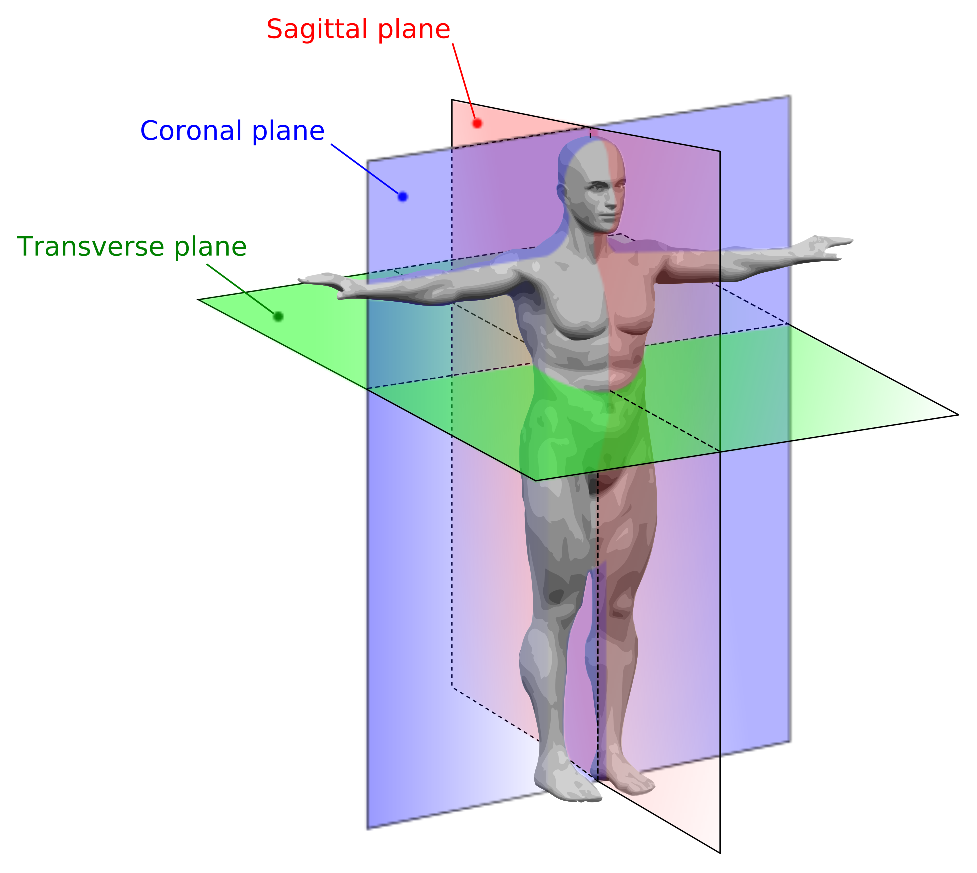
\includegraphics[width=0.5\textwidth]{spahittalPlae}
    \caption{Sagittal Plane}
    \label{fig:sgplane}
\end{center}
\end{figure}

As shown in Figure~\ref{fig:sgplane}, motion is projected into three spaces:the sagittal plane, coronal plane and transverse plane.
For bipedal walking,
 yaw and roll motion are relatively small and usually treated as secondary motion or totally neglected,  the main motion happens in the \emph{sagittal plane}.




Due to the above reason, this chapter focuses on the motions in sagittal plane, and  the motions of other \dof s in coronal plane and transverse plane are discussed in Chapter~\ref{chap:highdor}.
Such a simplification will not change the basic motion characteristics and adaptation tendency.
Since more {\dof}s will make the ``symmetry'' not so perfect and may cause confusions in explaining the idea, the discussions about more {\dof}s are delayed.



\subsection*{Dynamics}

The simplified walking model is shown in Figure~\ref{fig:passivekneewalker}.

\begin{figure}[!htbp]
  \begin{center}
    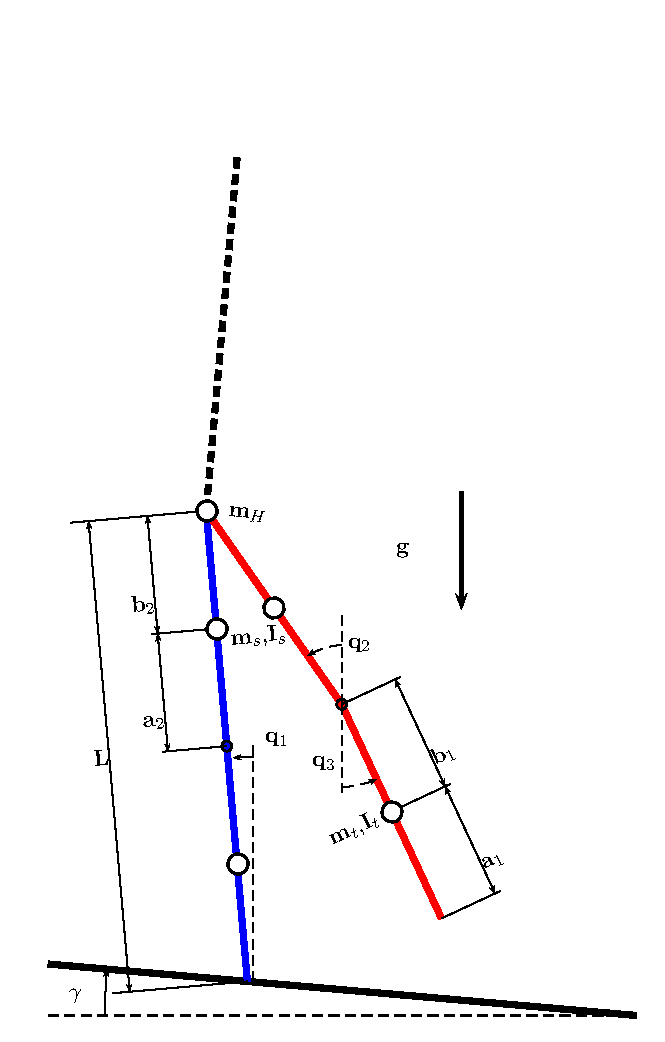
\includegraphics[height=0.4\textheight]{PWI}
    \caption{A Passive Walking Model with Knee}
    \label{fig:passivekneewalker}
  \end{center}
\end{figure}
The walking model of Figure~\ref{fig:passivekneewalker} is based on rigid body dynamics.
The supporting leg is kept straight.
In the figure, $L$ is the length of the leg, $q_1$ is the angle of the supporting leg,
$m_t$ and $m_s$ are the mass of the shank and thigh,
$q_2$ and $q_3$ are the corresponding angles of the swinging shank and thigh,
$b_1,a_1$ and $b_2,a_2$ describe the relative position of gravity center,
$m_h$ represents sum mass of the body and hip .






Like the bouncing ball system, this dynamic system is hybrid\citep{ames2006categorical} and includes both continuous and discrete dynamics.
Passive walking with knees includes four phases\citep{Chen2007}.
\begin{itemize}
\HiItem{Free Swing Phase}
The support leg (the blue one) is kept straight.
During this phase, the knee of the swing leg is bended, and the thigh and shank swing freely.
\HiItem{Knee Strike Phase}
The knee joint of the swing leg has a limit.
When the knee angle reaches the limit, a collision happens.
After the collision, the swing leg is kept straight.
\HiItem{Knee Lock Swing Phase}
During this swing phase, both the swing and support leg are kept straight.
\HiItem{Heel Strike Phase}
When the heel of the swing leg hits the ground, a collision happens.
After that the swing and support legs are switched.
\end{itemize}

Figure~\ref{fig:fwalkingphase} shows the gaits of four phases.
\begin{figure}[!htbp]
  \begin{center}
      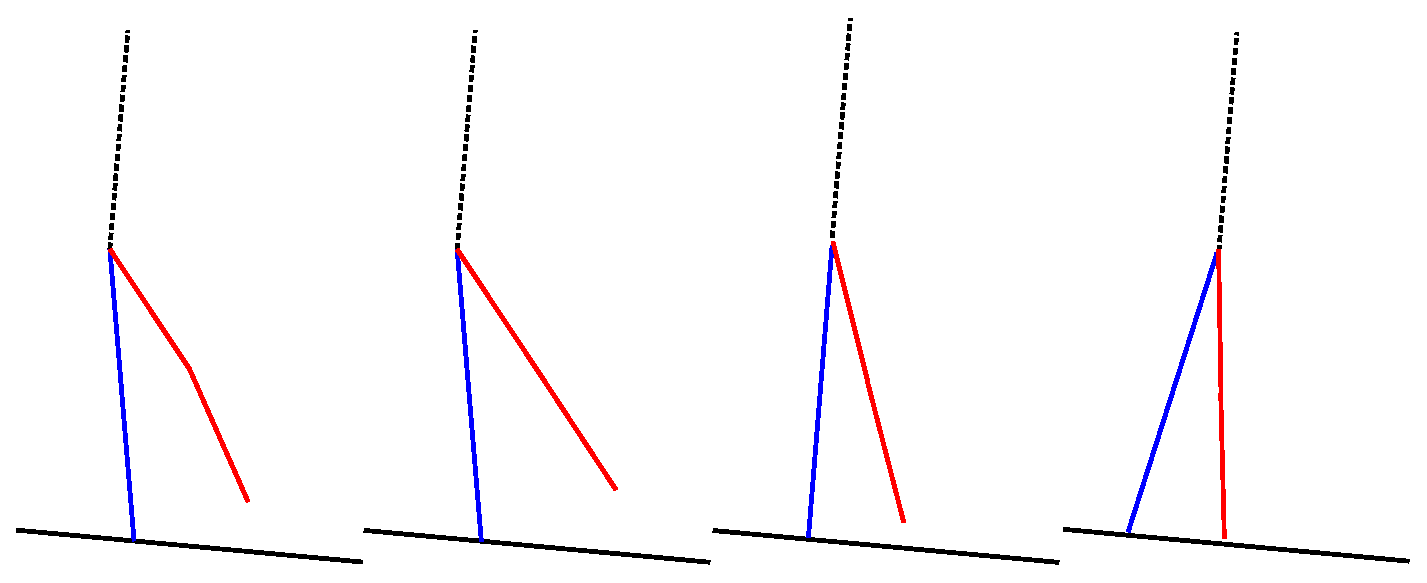
\includegraphics[width=0.7\textwidth]{Fourphase}
    \caption{The four phases in Walking}
    \label{fig:fwalkingphase}
\end{center}
\end{figure}





\begin{itemize}
\HiItem{Flying Phases}
Both the free and locked knee swing phases are described by the continuous dynamics.
Both equations are in the form of Equation~\ref{eq:flyequationpwi}.
\begin{equation}
\label{eq:flyequationpwi}
M(\mathbf{q}) \ddot{\mathbf{q}} + C(\mathbf{q,\qd})\dot{\mathbf{q}} + N(\mathbf{q}) = 0
\end{equation}
where $q=[q_1,q_2,q_3]$,$\qd=[\dot{q_1},\dot{q_2},\dot{q_3}]$,$M$ is the initial mass matrix,  and $C$ and $N$ are the centrifugal force matrix and gravity respectively. 
For Knee Free Phase,  $M$ and $C$ are $3$ by $3$ matrix, and $N$ is $3$ by $1$ vector.
for Knee Lock Phase, $M$ and $C$ are $2$ by $2$ matrix, and $N$ is $2$ by $1$ vector.
Putting them into the standard form, and define $\state=[q,\qd]$, Equation~\ref{eq:flyequationpwi} is transformed into Equation~\ref{eq:stateformpw}
Then the function is in the form.
\begin{equation}
\label{eq:stateformpw}
\dot{\state}=
-\left[ 
\begin{array}{cc}
\mathbf{1} &0\\
0 &M 
\end{array}
\right]^{-1}
\left[ 
\begin{array}{cc}
0 &\mathbf{1}\\
0 &C 
\end{array}
\right]\state
-\left[ 
\begin{array}{c}
\mathbf{0}\\
 N 
\end{array}
\right]
\end{equation}

\HiItem{The Strike Phases}
The knee strike and heel strike phases are modelled based on discrete dynamics.
Collision equations are developed based on momentum preserving principle.
Both collision equations are in the form of Equation~\ref{eq:collidequ}.
\begin{equation}
\label{eq:collidequ}
J^{+}\dot{\mathbf{q}}^{+} = J^{-}\dot{\mathbf{q}}^{-}
\end{equation}

where $J$ is the matrix of angular momentum inertia, and the superscripts~$+,-$ represent those after and before collision respectively.
For Knees Strike,$J^-$ is a $3$ by $2$ matrix, $J^+$ is $2$ by $2$ matrix;
For Heel Strike, both $J^{+,-}$ are $2$ by $2$ matrix.
\end{itemize}
Dynamic equations are developed based on Lagrange Mechanics~\citep{Goldstein2002}.
For details of calculating the dynamic equation, please refer to \citep{Chen2007}
For the components of each matrix, please refer to the appendix.


\begin{figure}[!htbp]
  \begin{center}
    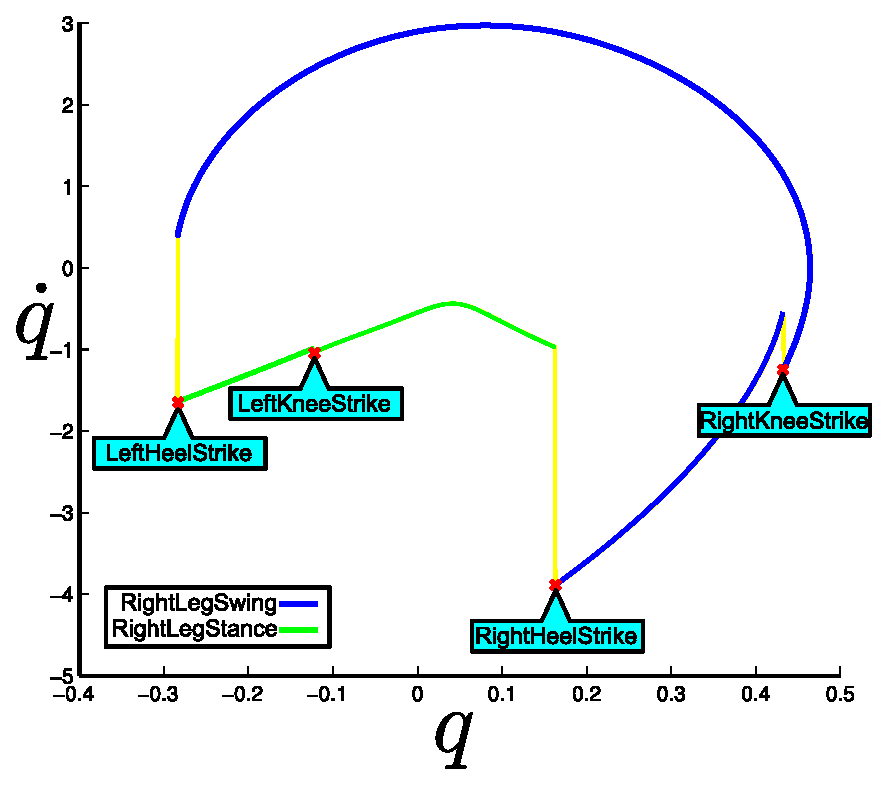
\includegraphics[width=0.7\textwidth]{walk_cycle_index}
    \caption{Four Phases Marked on a Walking Cycle}
    \label{fig:phasesmaker}
\end{center}
\end{figure}

With special initial conditions, the passive walker can walk down the slope with a stable gait.
On the phase plot,  a limit cycle emerges. 
Figure ~\ref{fig:phasesmaker} shows the phase plot of one thigh for a stable walking cycle.
where the events that separate the four phases are marked. 

In theory, the generalized coordinates for walking have $4$ degrees of freedom, with angle for shank and thigh for each leg.
Since the state space is $8$ dimension, it is not possible to draw the phase portrait on a $2$ dimension picture.
However, considering that motions of the two legs are almost the same, it is enough to show one leg motion, the state space is reduced to $4$ dimensions.
In the further analysis, we will indicate that the knee motion is not very important since the motion of the thigh captures the most valuable motion.
Thus we only draw the phase plot of the thigh of one leg.
Figure ~\ref{fig:phasesmaker} only shows the motion of the right leg.
The green plot shows the stance phase. 
During this phase, the right leg is supporting the body.
The blue parts show the swing phase.
During this phase,  the right leg is swinging and the left leg is supporting the body.
The yellow lines mark the $4$ collision events during walking.
Note that during the collision, the walking dynamic is discontinuous, and the speed of walking is changed suddenly without changing the position.
This means the yellow segments are not on the limit cycle. 
If the walker starts from the state in the middle of the yellow segment, it will fall.











\section{Global Motor Control and Adaptive Gaits}
The Passive Dynamic Walker exhibits a natural looking gait.
However, the walking motion is not stable.
In \moit, the repetitive walking motion suggests that the natural walking dynamic forms a limit cycle.
It seems that humans utilize the limit cycle for walking,  results in high energy efficiency.

To overcome the fragile stability, \cpg\ is applied with the hope to make the walking more stable through entrainment.
Experiments have shown that stability is enhanced and different perturbations result in varied and natural looking responsive motions.




\subsection{Entrainment}
For walking, only one neural oscillator is applied to maintain the stability of limit cycle.
The output of neural oscillator works as torque applied to hip angel (angle between the two thighs).
The dynamics are shown in Equation~\ref{eq:neuralwalk}
\begin{equation}
\label{eq:neuralwalk}
M(\mathbf{q}) \ddot{\mathbf{q}} + C(\mathbf{q,\qd})\dot{\mathbf{q}} + N(\mathbf{q}) = D\uout
\end{equation}
For the knee lock phase, $D=[1,-1]^T$.
For the knee free phase, $D=[1,-1,0]^T$.
This means the neural oscillator controls the thigh, and the knee is left to swing freely.

The input signal is the hip angle.
We have 
\[
	\uin=\hin(q_1-q_2)
\]





\begin{figure}[!htbp]
  \begin{center}
    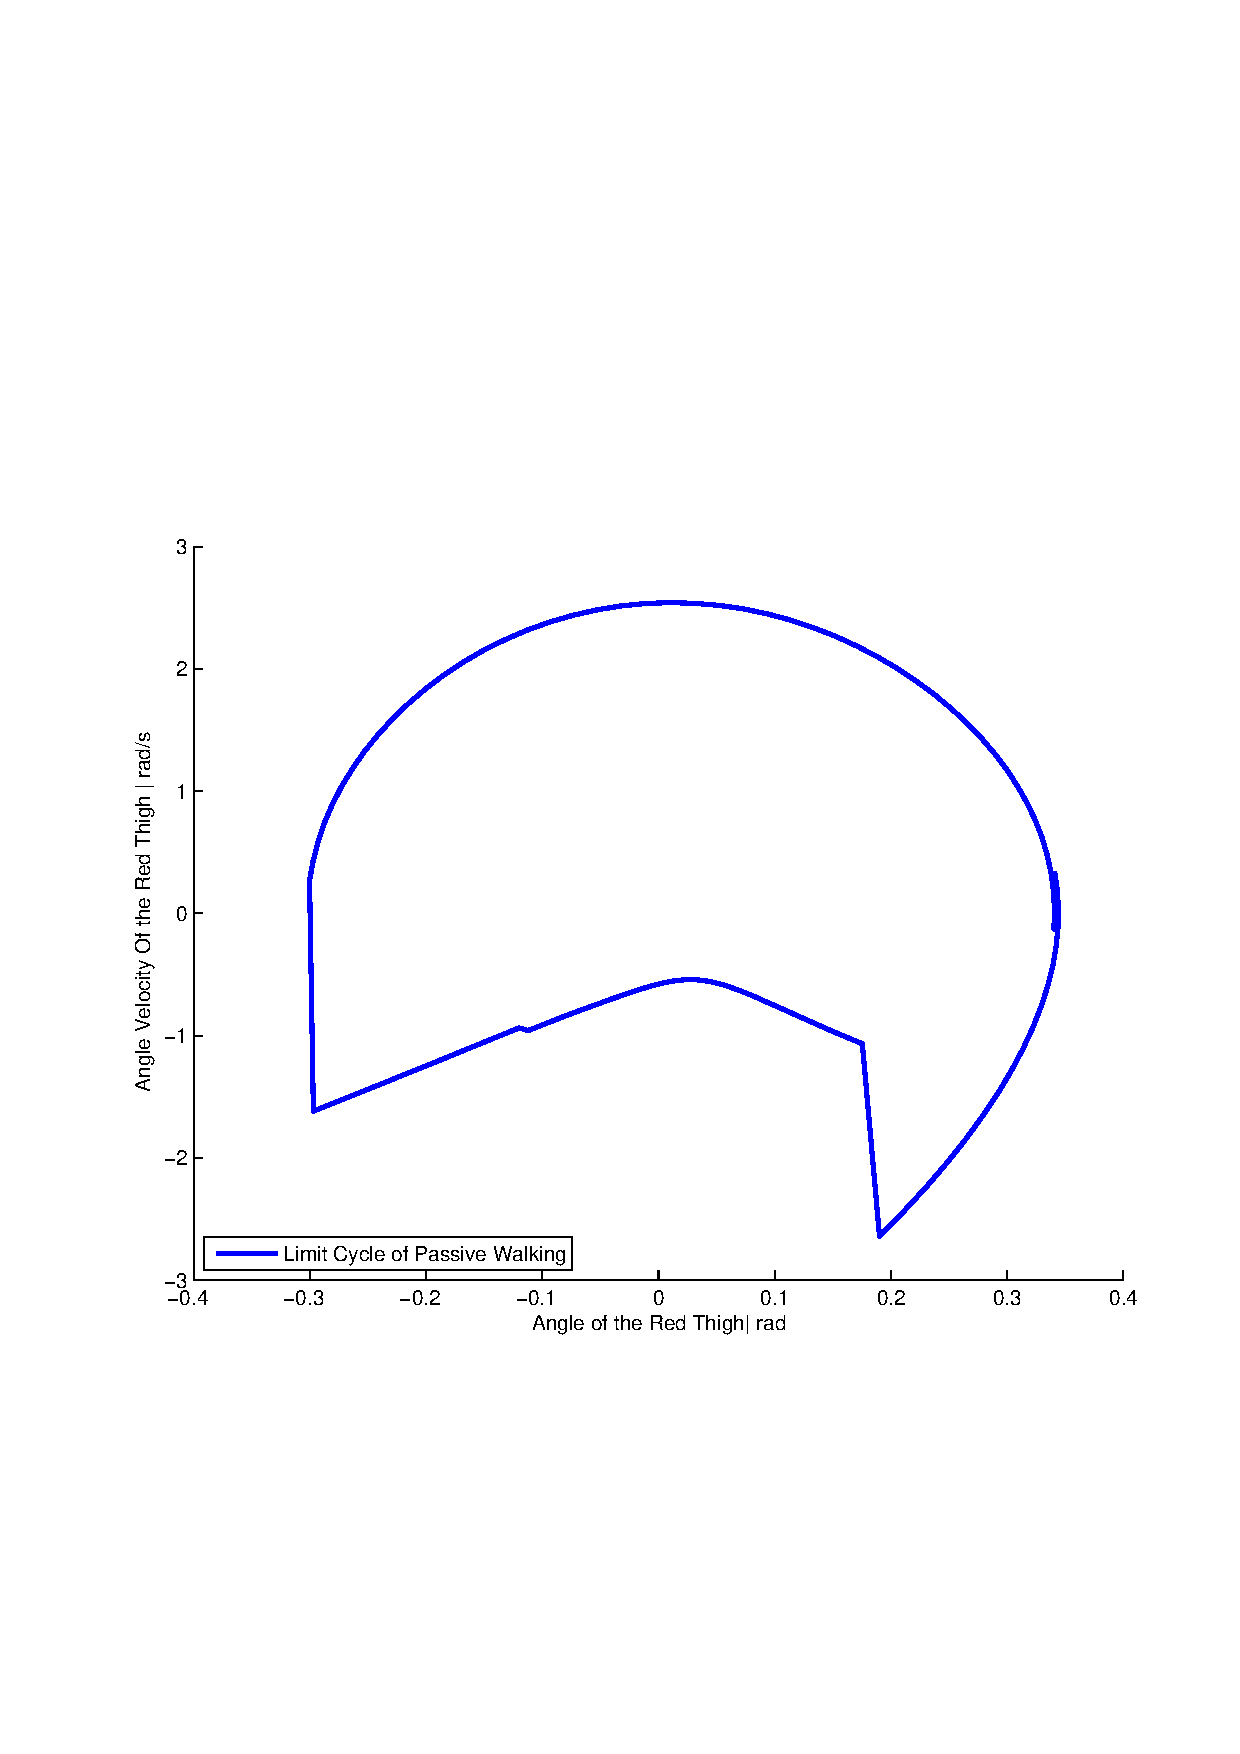
\includegraphics[width=0.5\textwidth]{PassiveWalkingLimitCycle}
    \caption{Limit Circle And Different Phase in Passive Walking}
    \label{fig:passivegaitlimitcycle}
\end{center}
\end{figure}


\begin{figure}[!htbp]
  \begin{center}
      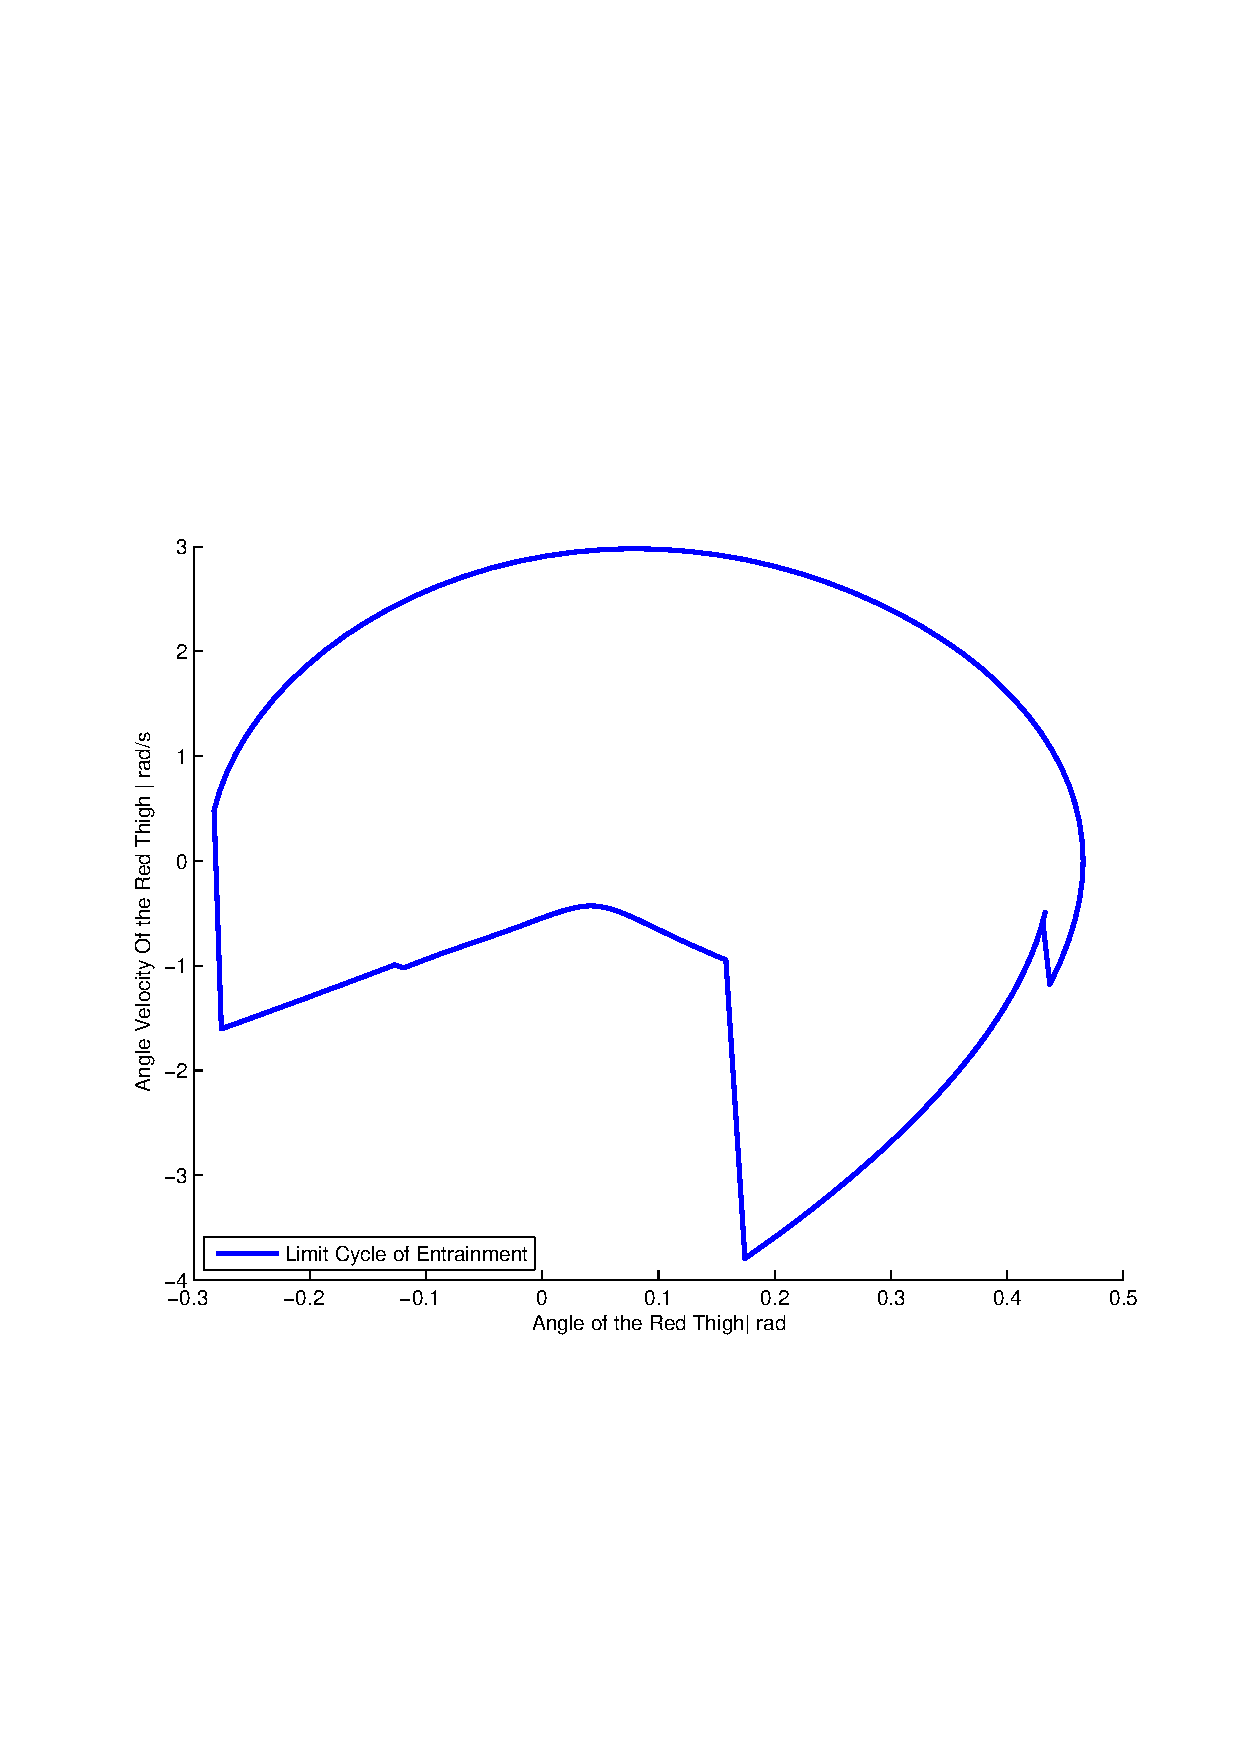
\includegraphics[width=0.5\textwidth]{NeuralWalkingLimitCycle}
    \caption{The gait with neural controller}
    \label{fig:entrainmentgaitlimitcyle}
\end{center}
\end{figure}
When the drive force is small, the limit cycle of entrainment system is similar to the original passive one.
Both limit cycles are shown in Figure~\ref{fig:passivegaitlimitcycle} and Figure~\ref{fig:entrainmentgaitlimitcyle}.
Walking gaits are shown in Figure~\ref{fig:entrainmentgait} and Figure~\ref{fig:passivegait}.
Both figures are sampled by the same time interval.
The controlled gait looks a little sparser.
It means that with the neural control input, the character walks a bit quicker. 




\begin{figure}[!htbp]
  \begin{center}
     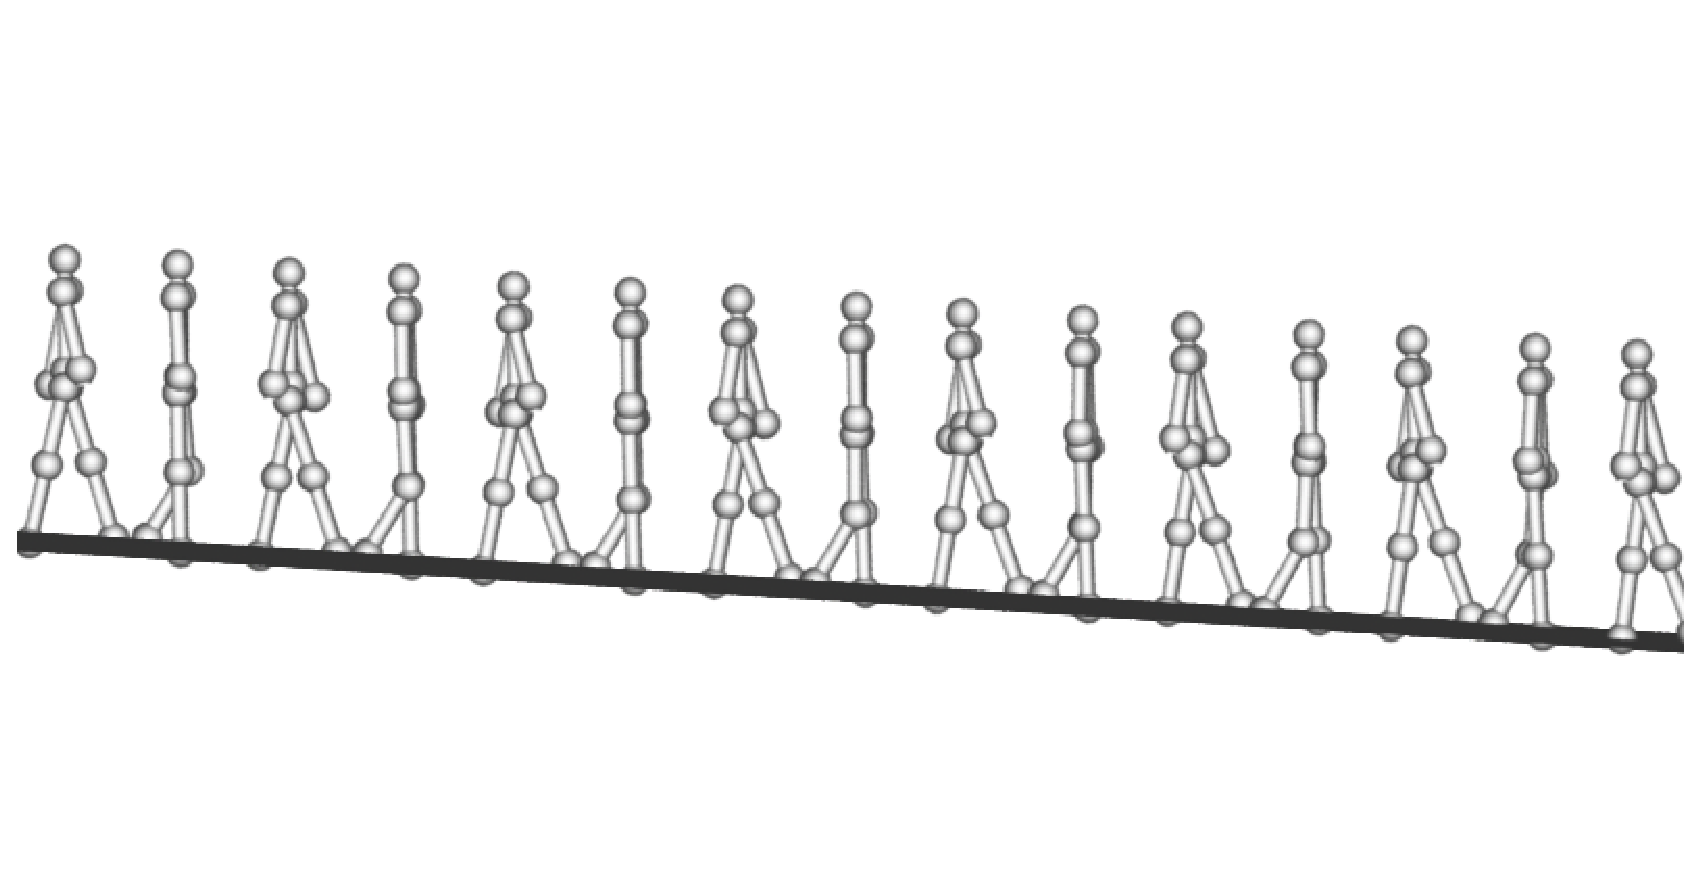
\includegraphics[width=0.7\textwidth]{PassiveGait}
    \caption{The Passive Walking Gait}
    \label{fig:passivegait}
\end{center}
\end{figure}

\begin{figure}[!htbp]
  \begin{center}
     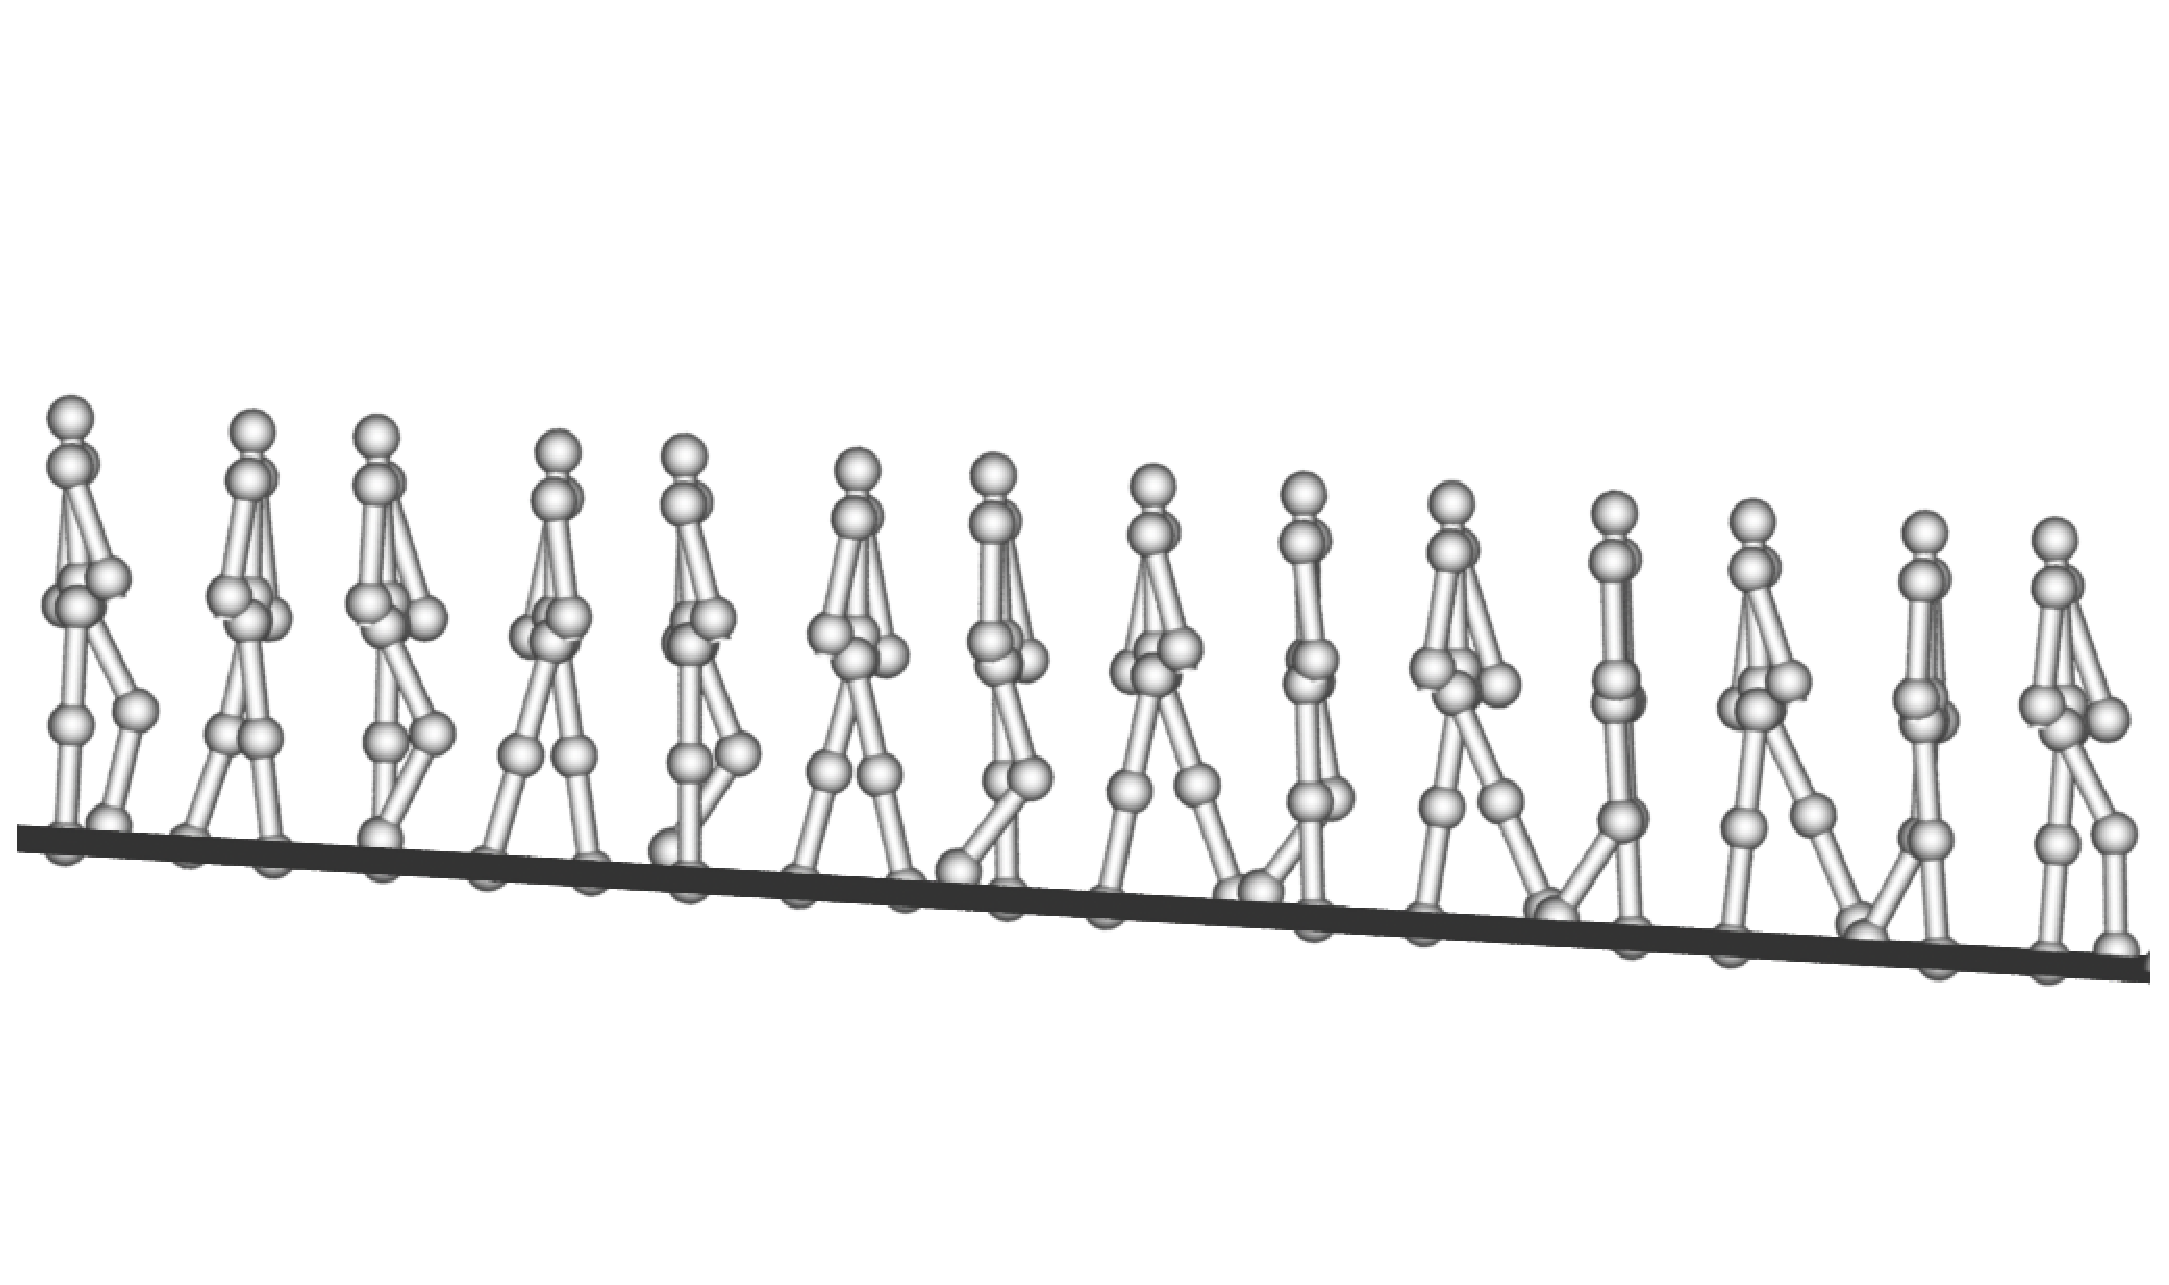
\includegraphics[width=0.7\textwidth]{neuralWalk}
    \caption{Passive Walking with Neural Control}
    \label{fig:entrainmentgait}
\end{center}
\end{figure}

By comparing the limit cycles and the walking gaits, we find out that the controlled gait and passive gait are quite similar.
The controlled gaits are a bit faster and the step size is  slightly bigger.
Visually, the two gaits are almost the same.
Although both are natural looking and very hard to detect control effort, the dynamics has been changed greatly, especially the stability.



\subsubsection*{Structural Stability}
Entrainment boosts the structural stability of walking. 
The passive walking can not be maintained on plane, because such a structure perturbation of slope angle has violated the topology.
The consequence is that limit cycle does not exist any more.


When passive walker walks on a plane, the step-size decreases after each step.
After several steps, the walker will stop or fall over, as shown in Figure~\ref{fig:passivegaitplane}.

After coupling with a neural oscillator, the  walker maintain walking with a small step size, as shown in Figure~\ref{fig:neuralwalkinggait}.
To maintain the energy efficient property of natural motion, $\uout$ is limited to small, leading to a small step size accordingly.

\begin{figure}[!htbp]
  \begin{center}
    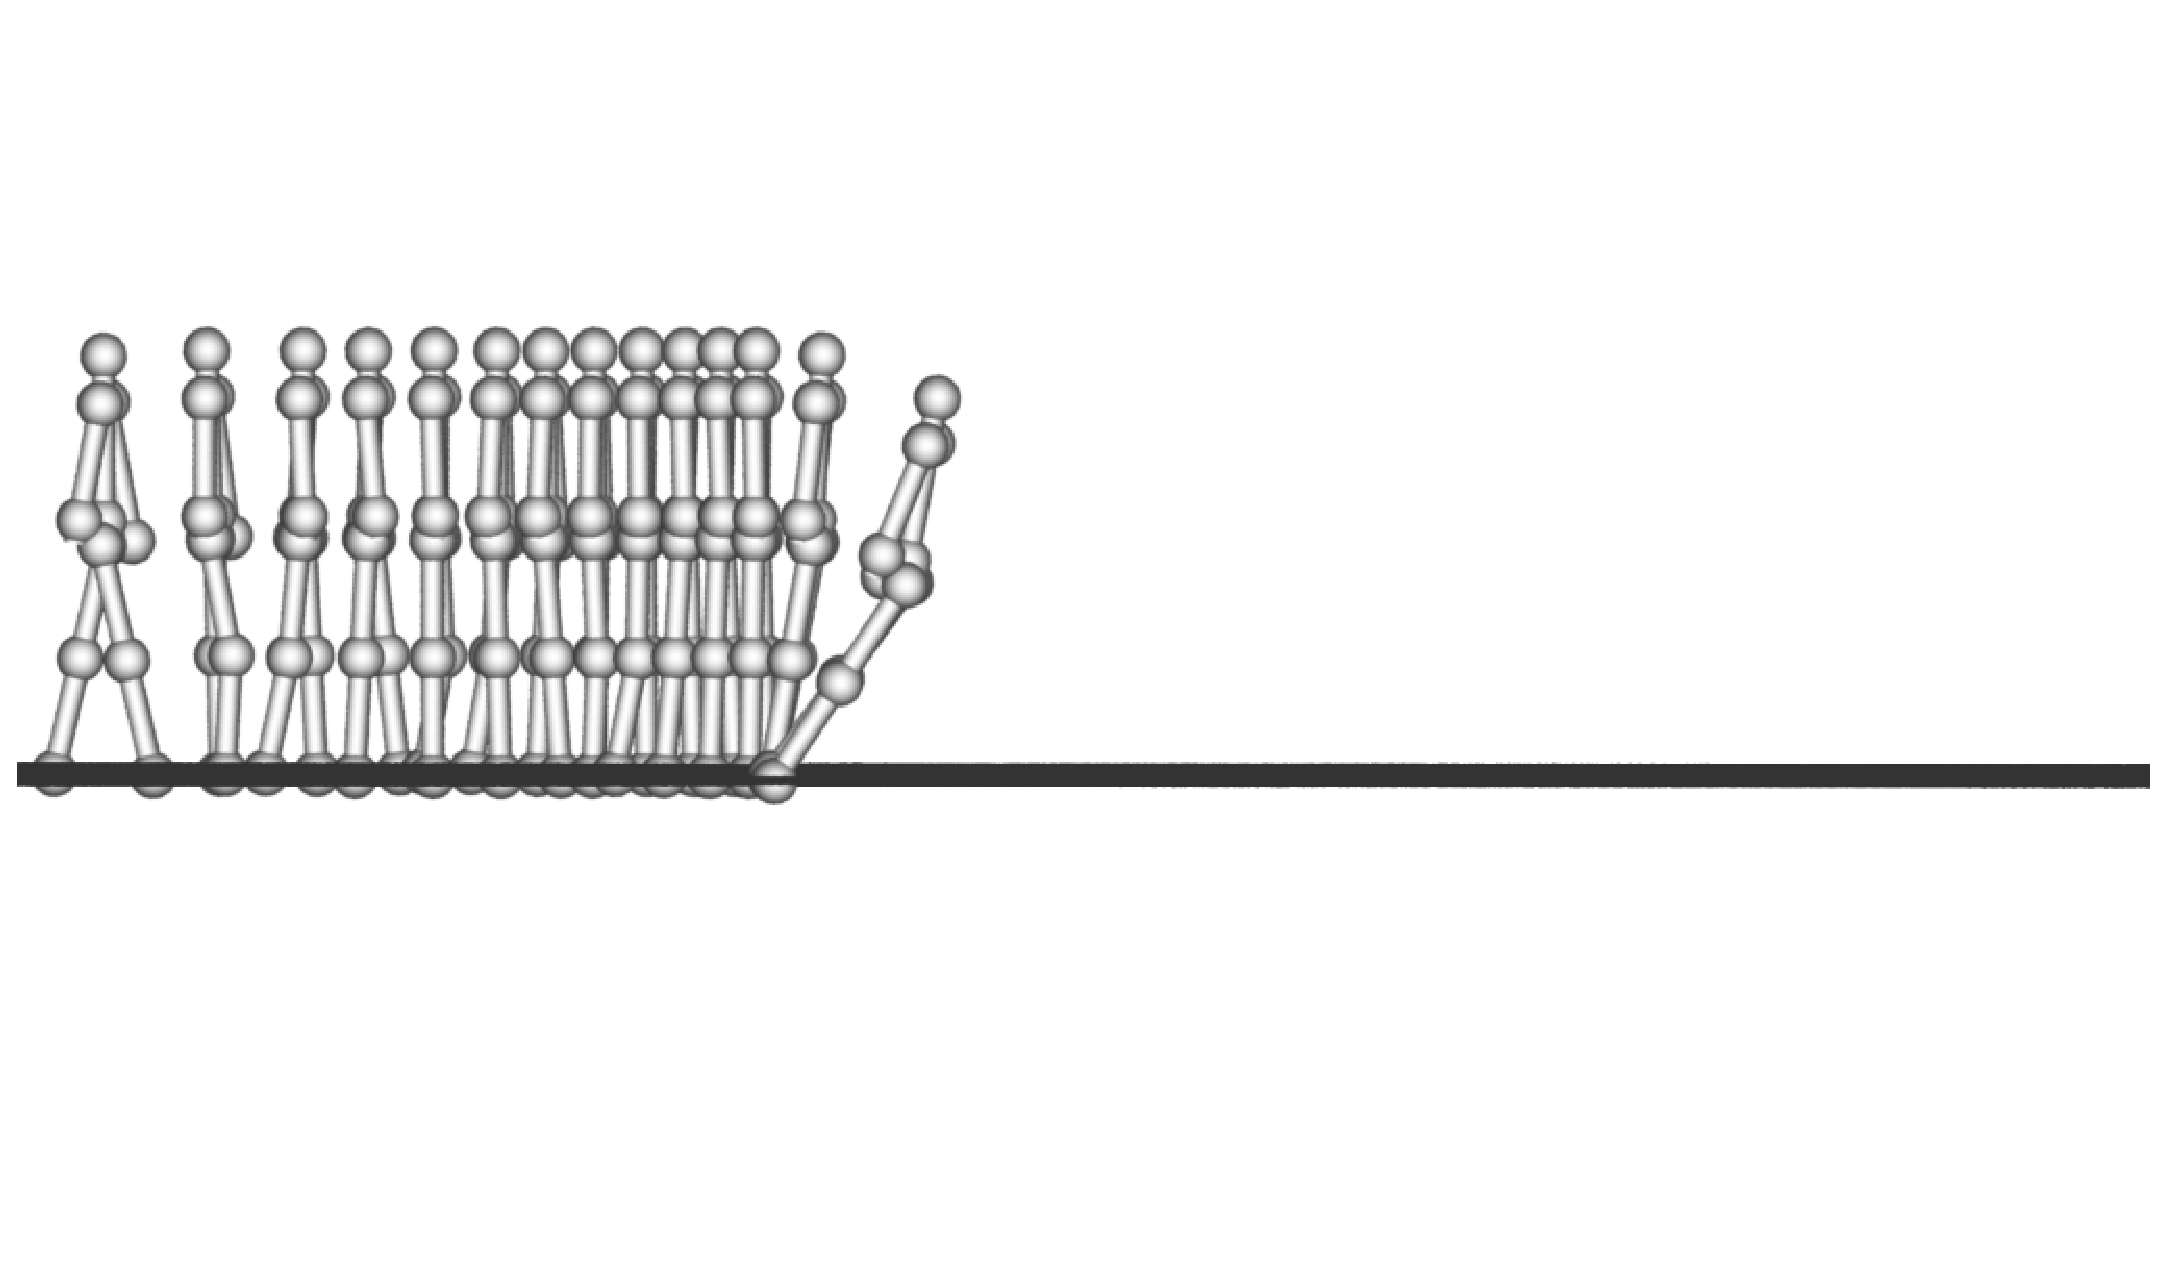
\includegraphics[width=0.7\textwidth]{PassiveOnPlane}
    \caption{The Passive Gait On Plain}
    \label{fig:passivegaitplane}
\end{center}
\end{figure}

\begin{figure}[!htbp]
  \begin{center}
     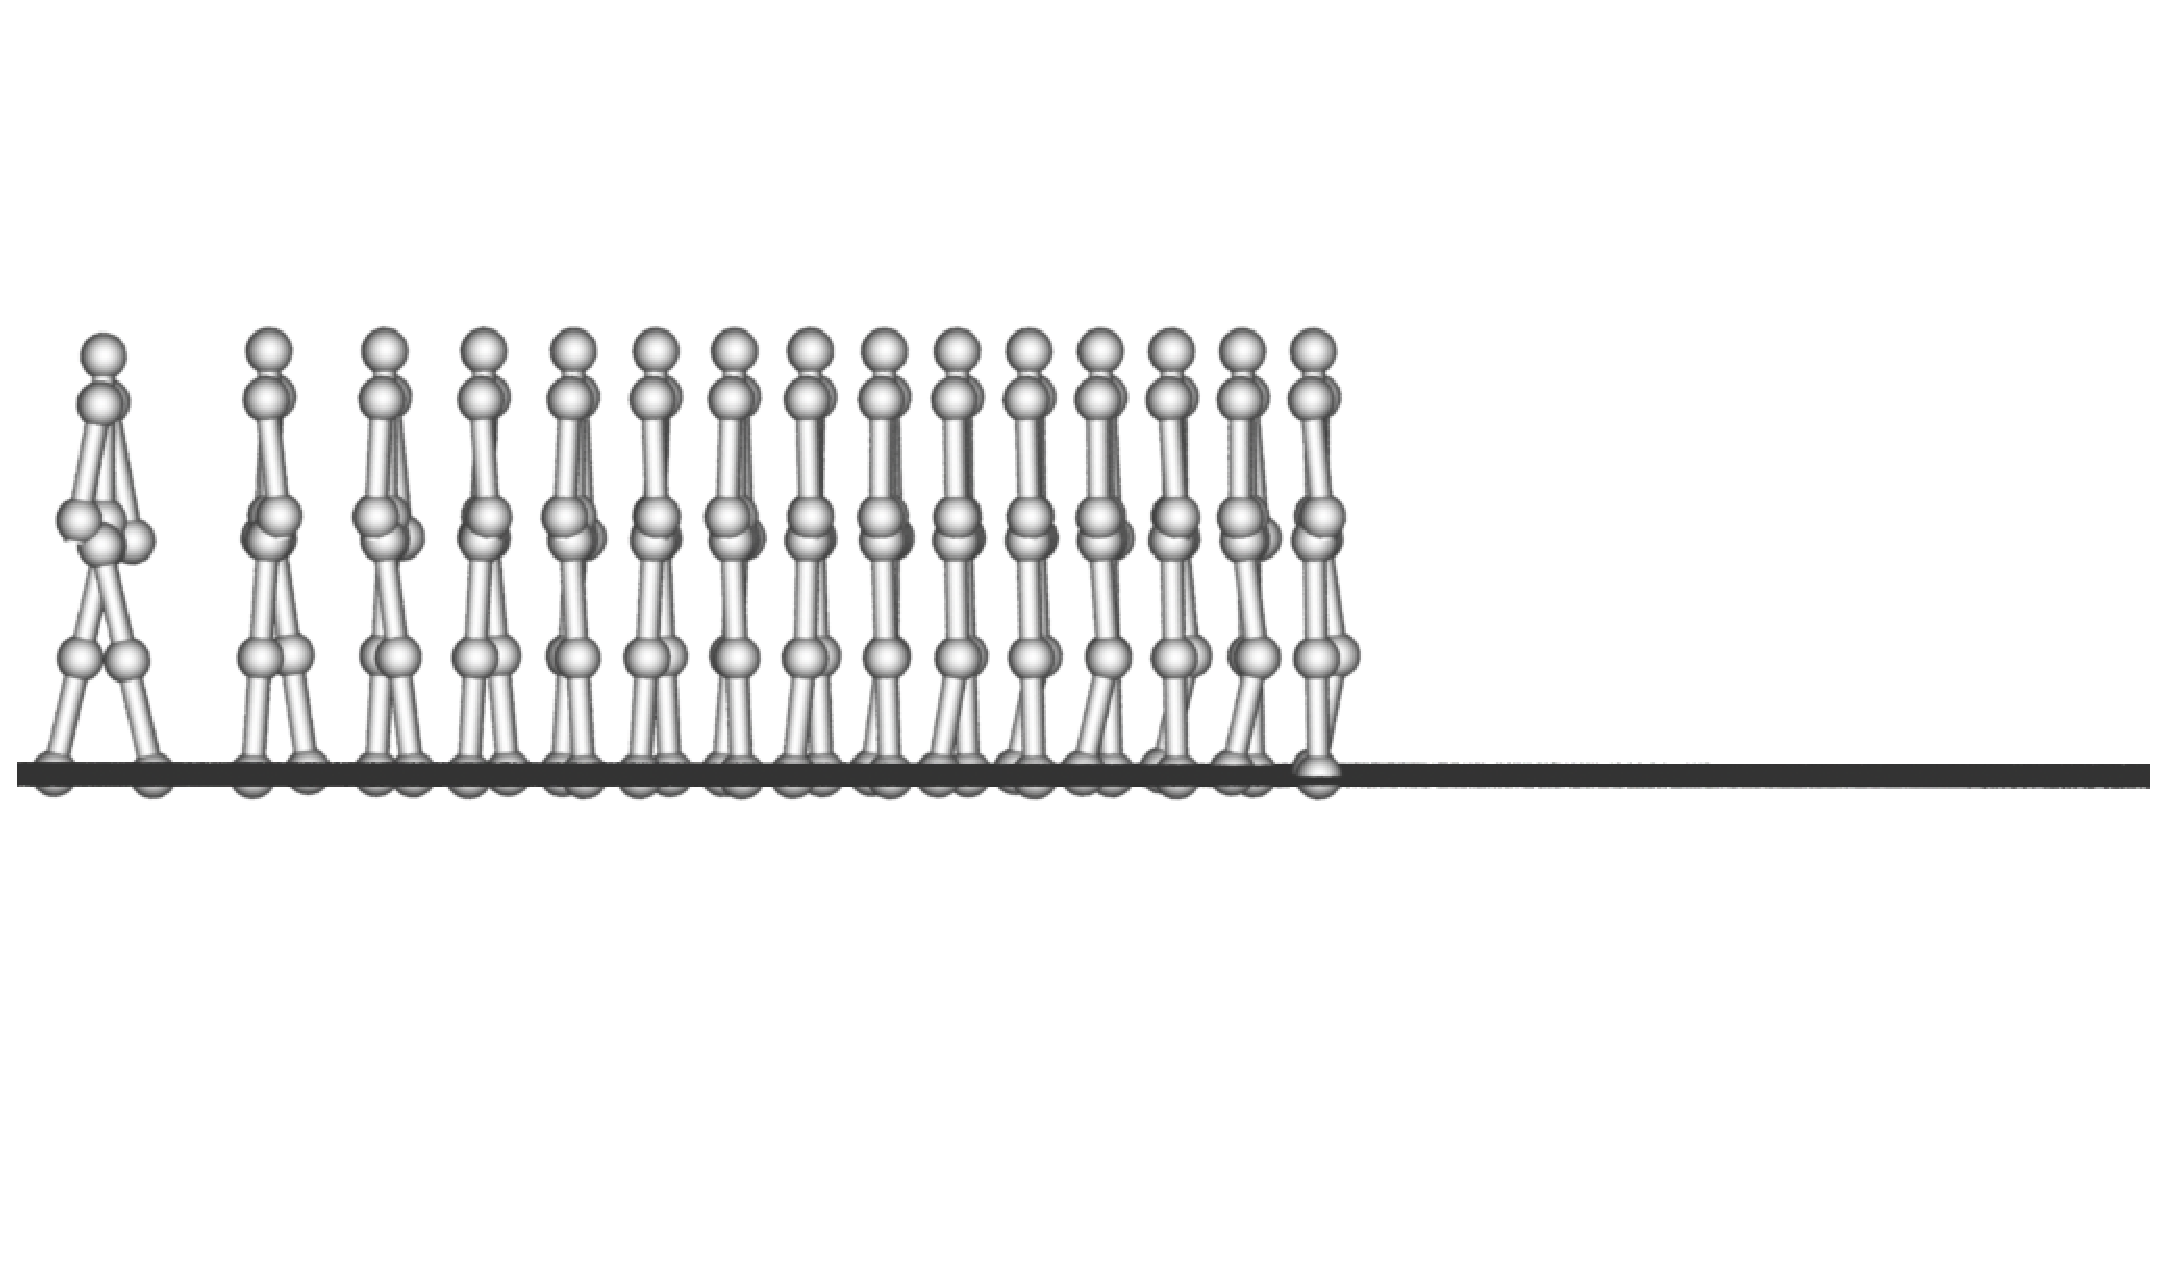
\includegraphics[width=0.7\textwidth]{NeuralWalkingPlane}
    \caption{Entrainment Gait On Plane}
    \label{fig:neuralwalkinggait}
\end{center}
\end{figure}

\begin{figure}[!htbp]
  \begin{center}
      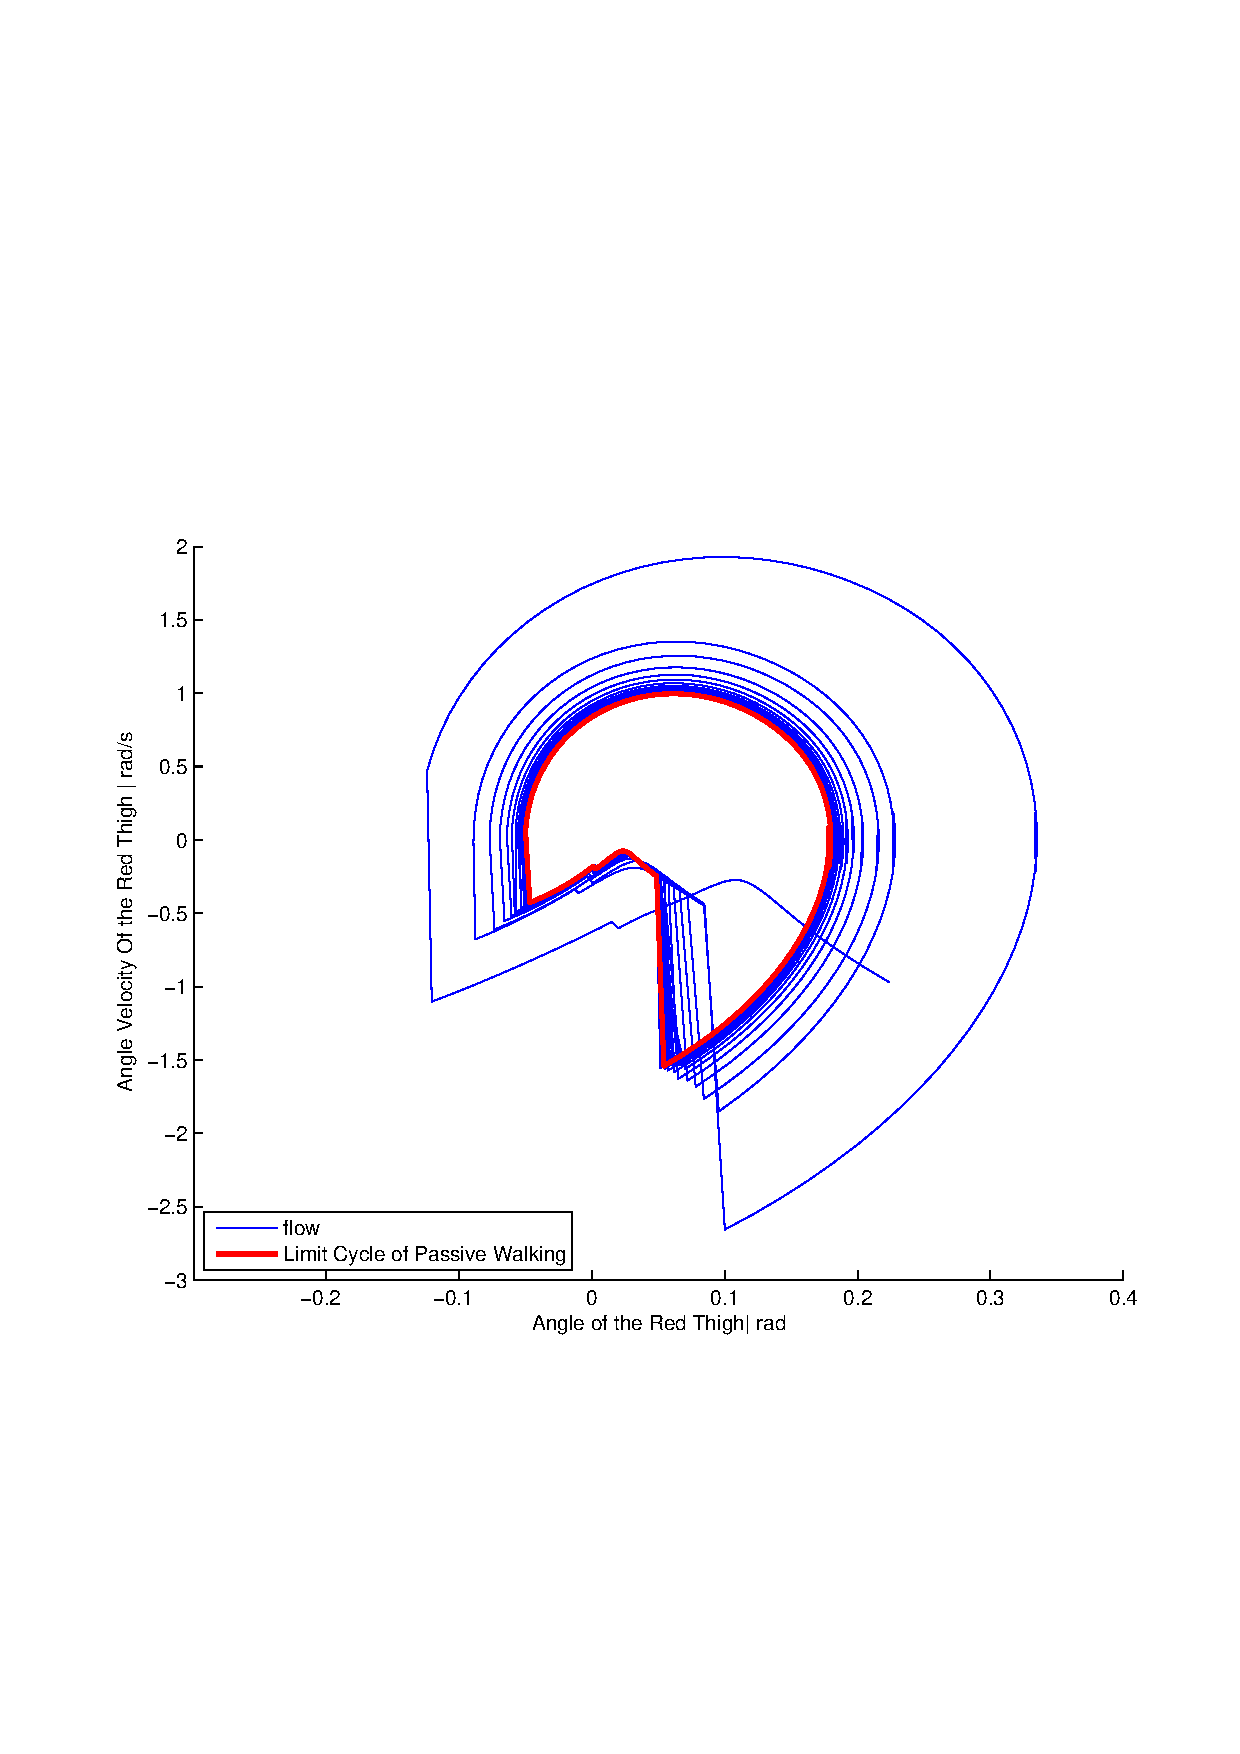
\includegraphics[width=0.7\textwidth]{NeuralPlaneCycle}
    \caption{Limit Cycle of entrainment gait on plane}
    \label{fig:entrainmentLimitCycleOnPlane}
\end{center}
\end{figure}

In Figure~\ref{fig:entrainmentLimitCycleOnPlane}, the walking cycle is kept shrinking over time, resulting in a gaits of walking to stop intention. 
But after several steps, the walking gaits reach a limit cycle (shown in red). 
The new walking limit cycle is of a smaller size, which means a smaller step.


\subsubsection*{Area of Basin of Attraction}
Another measurement for stability is to size of the basin of attraction.
Passive walking is fragile, which means the basin of attraction is very narrow.
If the walker is pushed, it will fall.

Entrainment greatly enlarges the basin of attraction of the walking limit cycle.
In Figure~\ref{fig:entrainmentLimitCycleOnPlane}, the initial position is far from the limit cycle.
It indicates that the basin of attraction has been enlarged.

A better test is to push or pull the walking character.
When push and pull are applied to the character, the state is moved away from the limit cycle.
The harder the push or the pull is, the further it moves away.
The gaits of  being pushed or pulled are shown in Figure~\ref{fig:PushGait} and Figure~\ref{fig:PullGait}.
For both cases, the characters start walking with normal stable gaits.
When the character is pushed forward, the character will take a big step and then slowly return to the normal step.
When the character is pulled backward, the character will take a smaller step or even step backwards for one or two step, and  gradually return to the normal walking gait.


\begin{figure}[!htbp]
  \begin{center}
      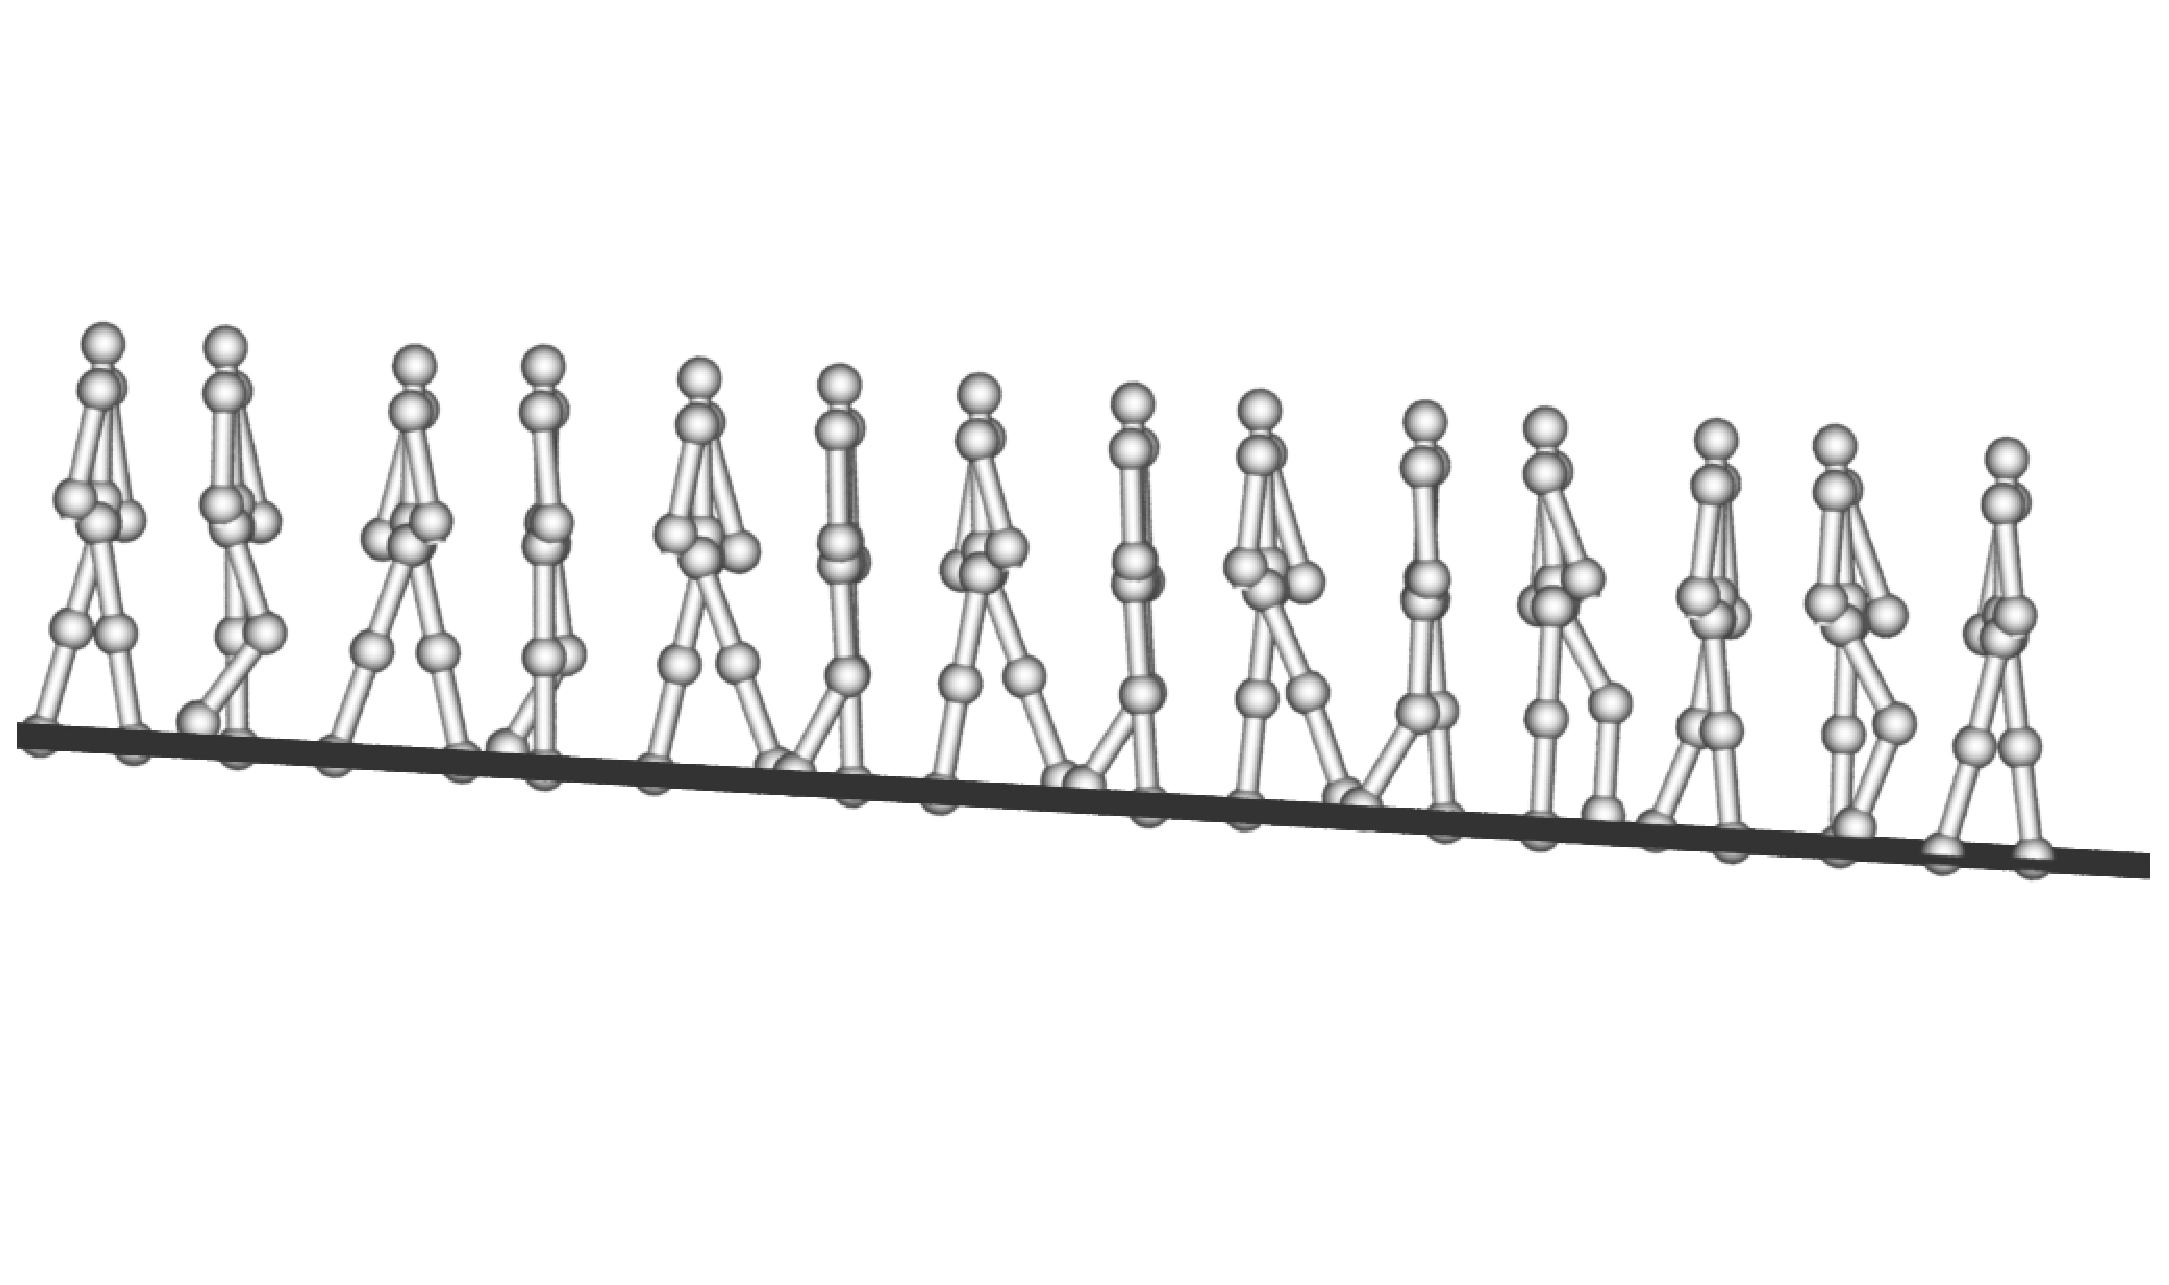
\includegraphics[width=0.7\textwidth]{PushGait}
    \caption{The Push Perturbated Gait}
    \label{fig:PushGait}
\end{center}
\end{figure}


\begin{figure}[!htbp]
  \begin{center}
      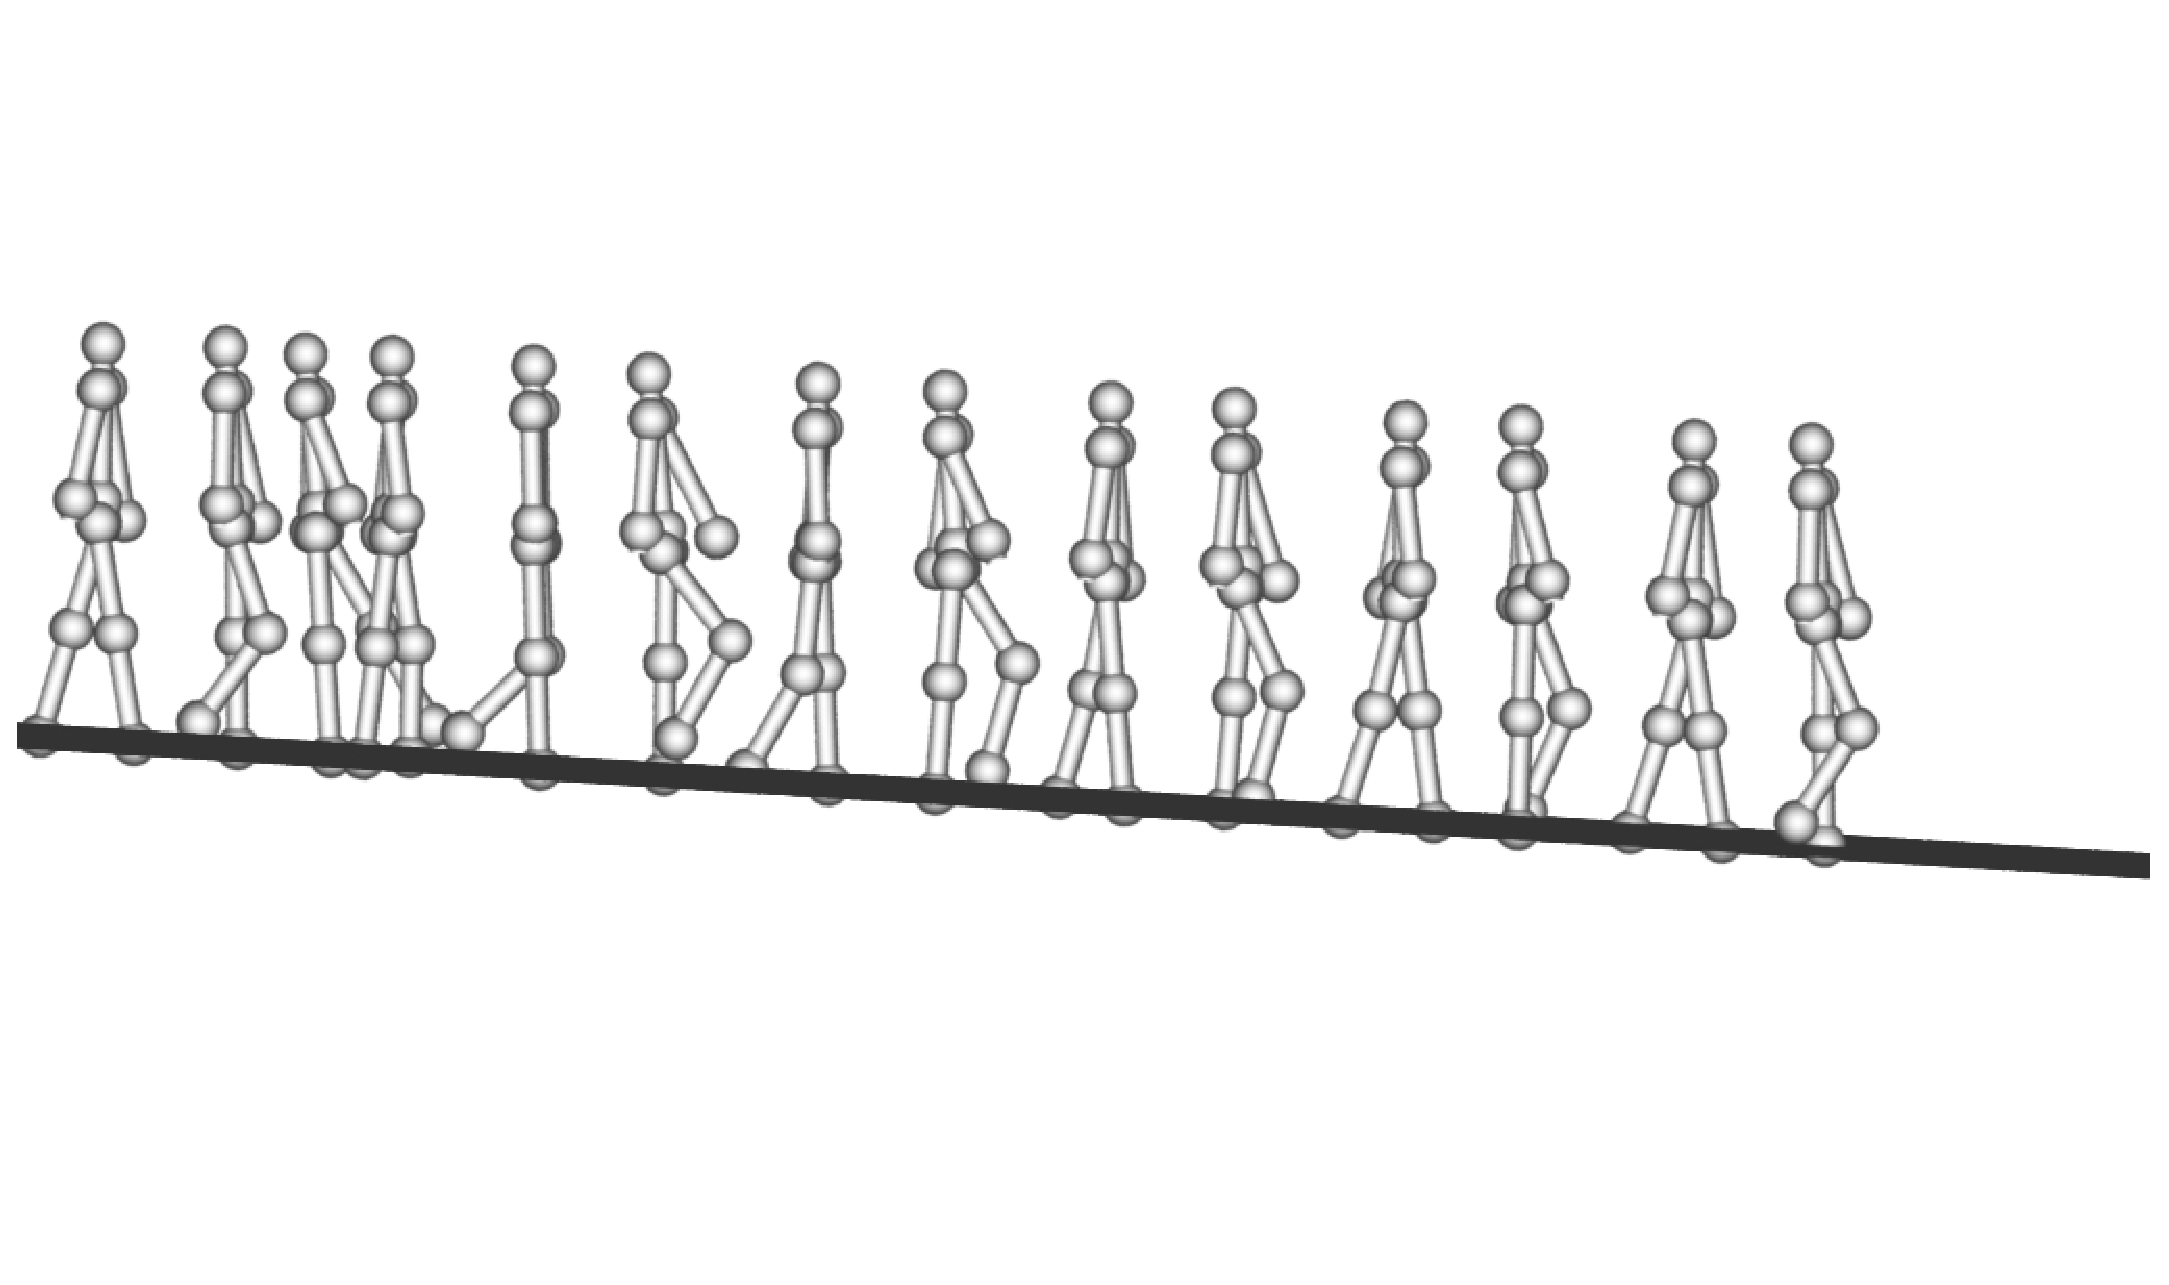
\includegraphics[width=0.7\textwidth]{PullGait}
    \caption{The Pull Perturbated Gait}
    \label{fig:PullGait}
\end{center}
\end{figure}

Figure~\ref{fig:PushGaitPlot} and Figure~\ref{fig:PullGaitPhasePlot} show the flow converging towards the limit cycle.
When the character is pushed, it takes a big walking cycle. 
However because of the entrainment, the walking cycle shrinks and trembles around the limit cycle. 
The pull effects make the character take a smaller step size in the next several steps.
The walker takes a bigger or smaller step to adjust walking and finally returns to the normal walking gait.


\begin{figure}[!htbp]
  \begin{center}
      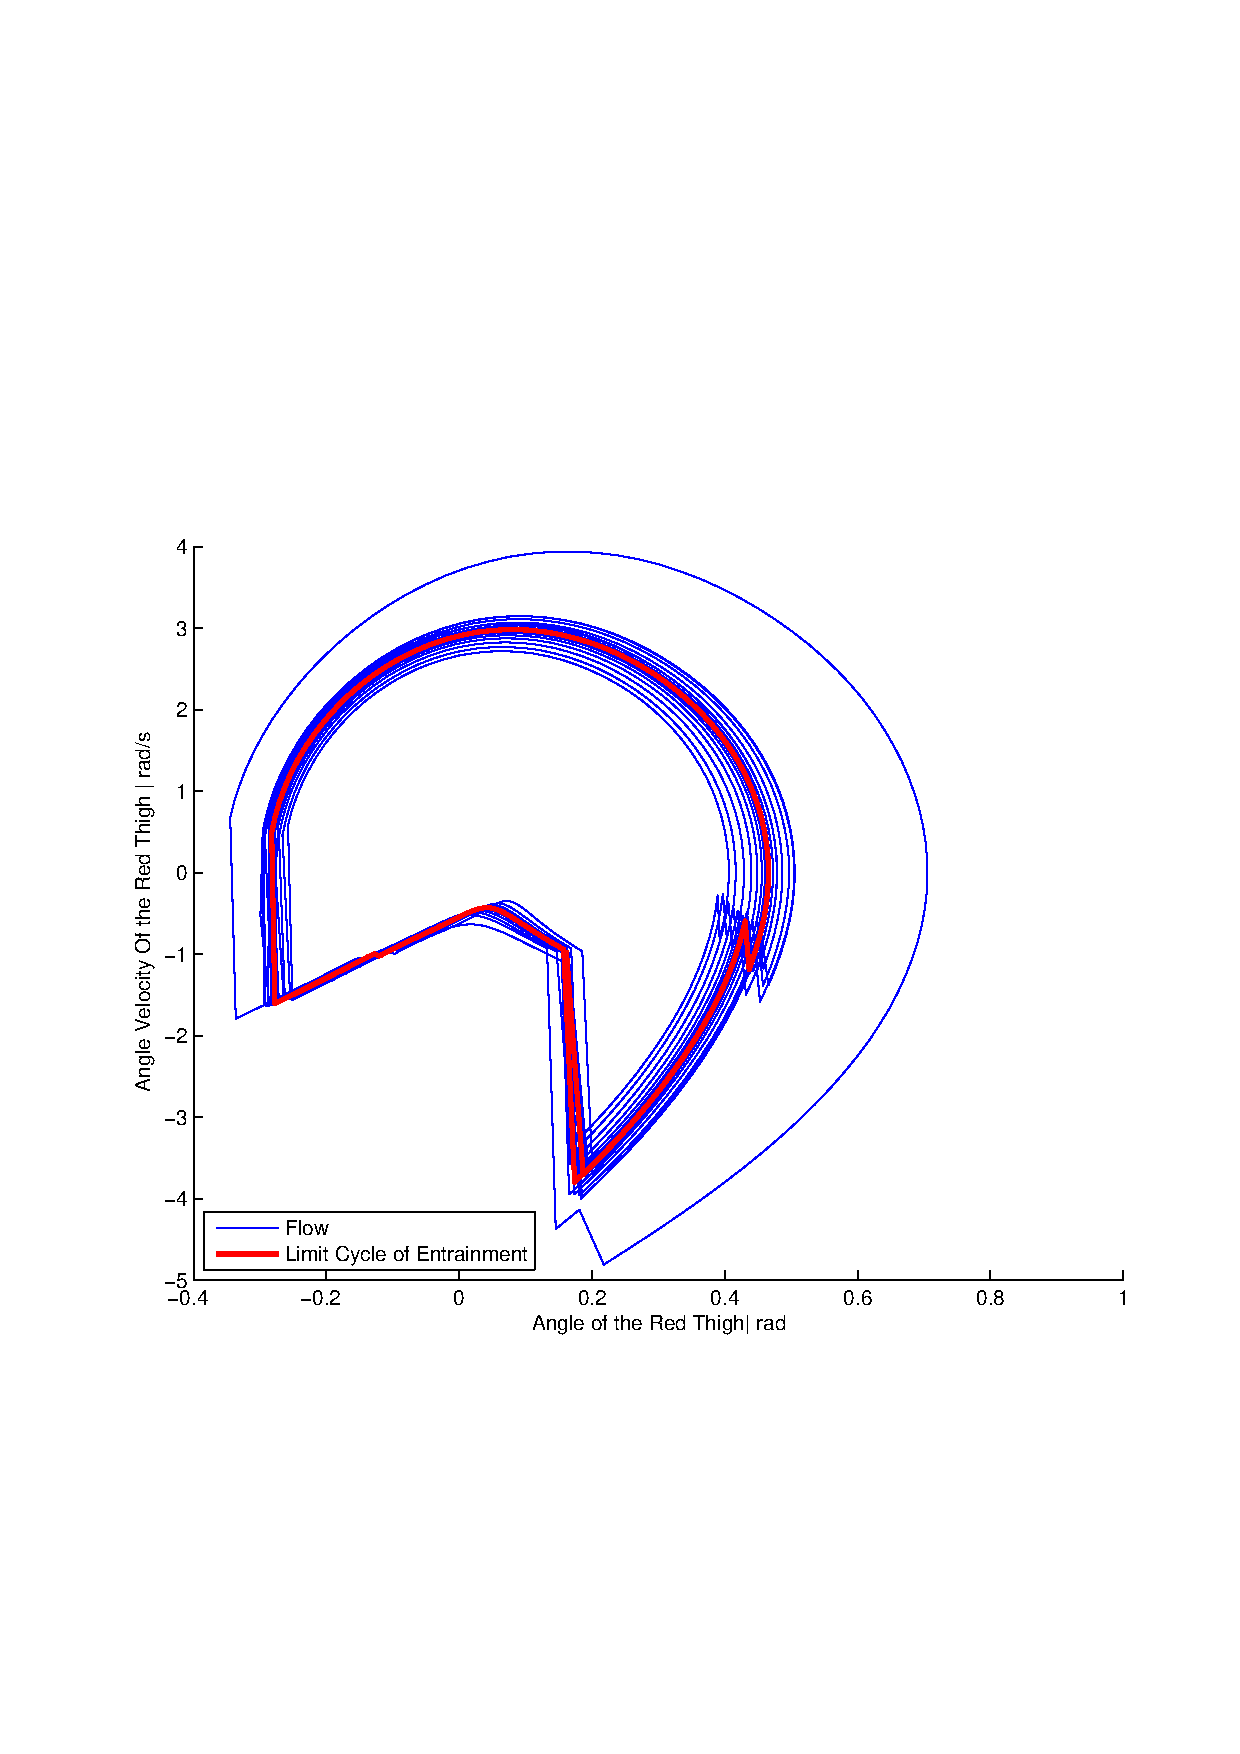
\includegraphics[width=0.7\textwidth]{PushWalkingPhasePlot}
    \caption{The Pushed Gait Phase Plot}
    \label{fig:PushGaitPlot}
\end{center}
\end{figure}


\begin{figure}[!htbp]
  \begin{center}
      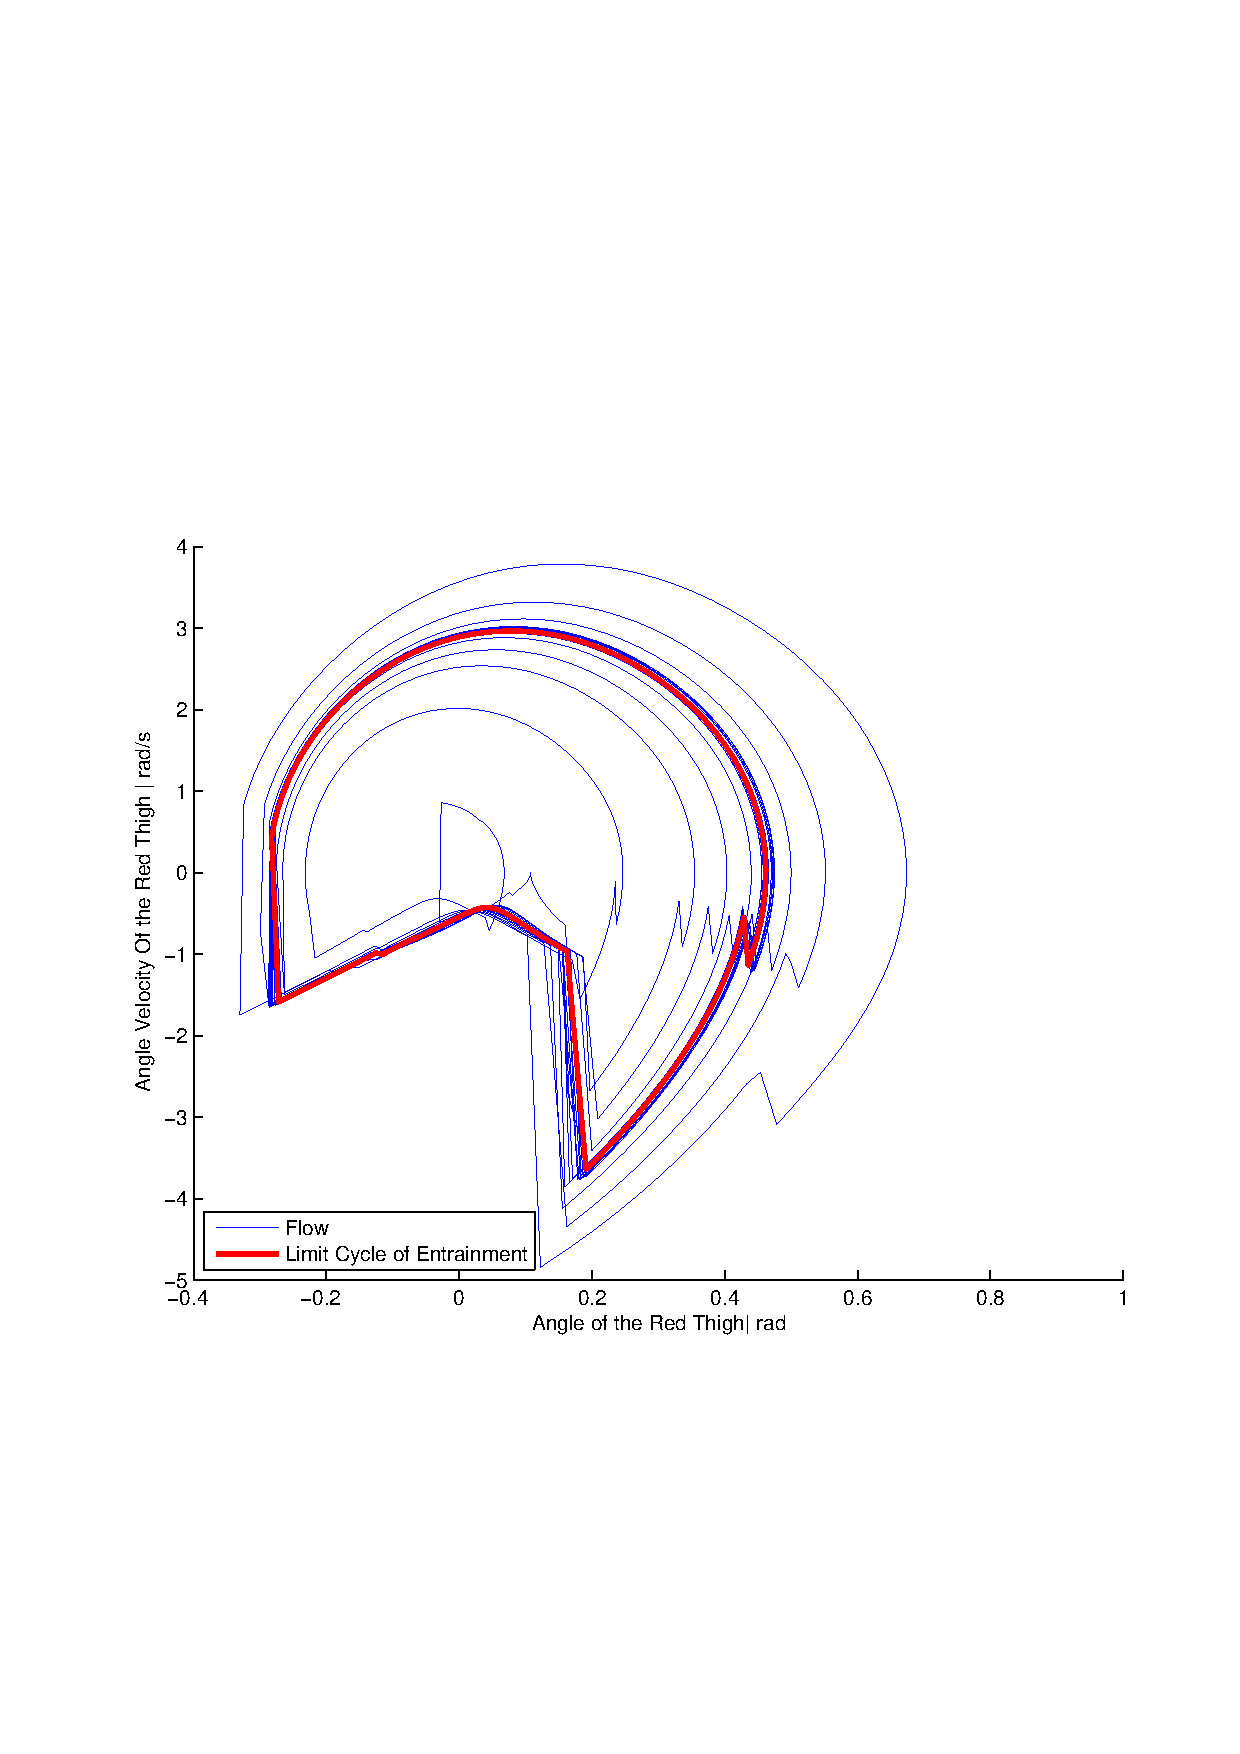
\includegraphics[width=0.7\textwidth]{PullWalkingPhasePlot}
    \caption{The Pulled Gait Phase Plot}
    \label{fig:PullGaitPhasePlot}
\end{center}
\end{figure}


The initial step size can also be changed, and the walker will adjust it automatically.
Figure~\ref{fig:bigStepIni} and Figure~\ref{fig:smallStepini} show the gaits.
Figure~\ref{fig:bigstepiniGaitPlot} and Figure~\ref{fig:smallstepiniPhasePlot} show the phase plots.

\begin{figure}[!htbp]
  \begin{center}
      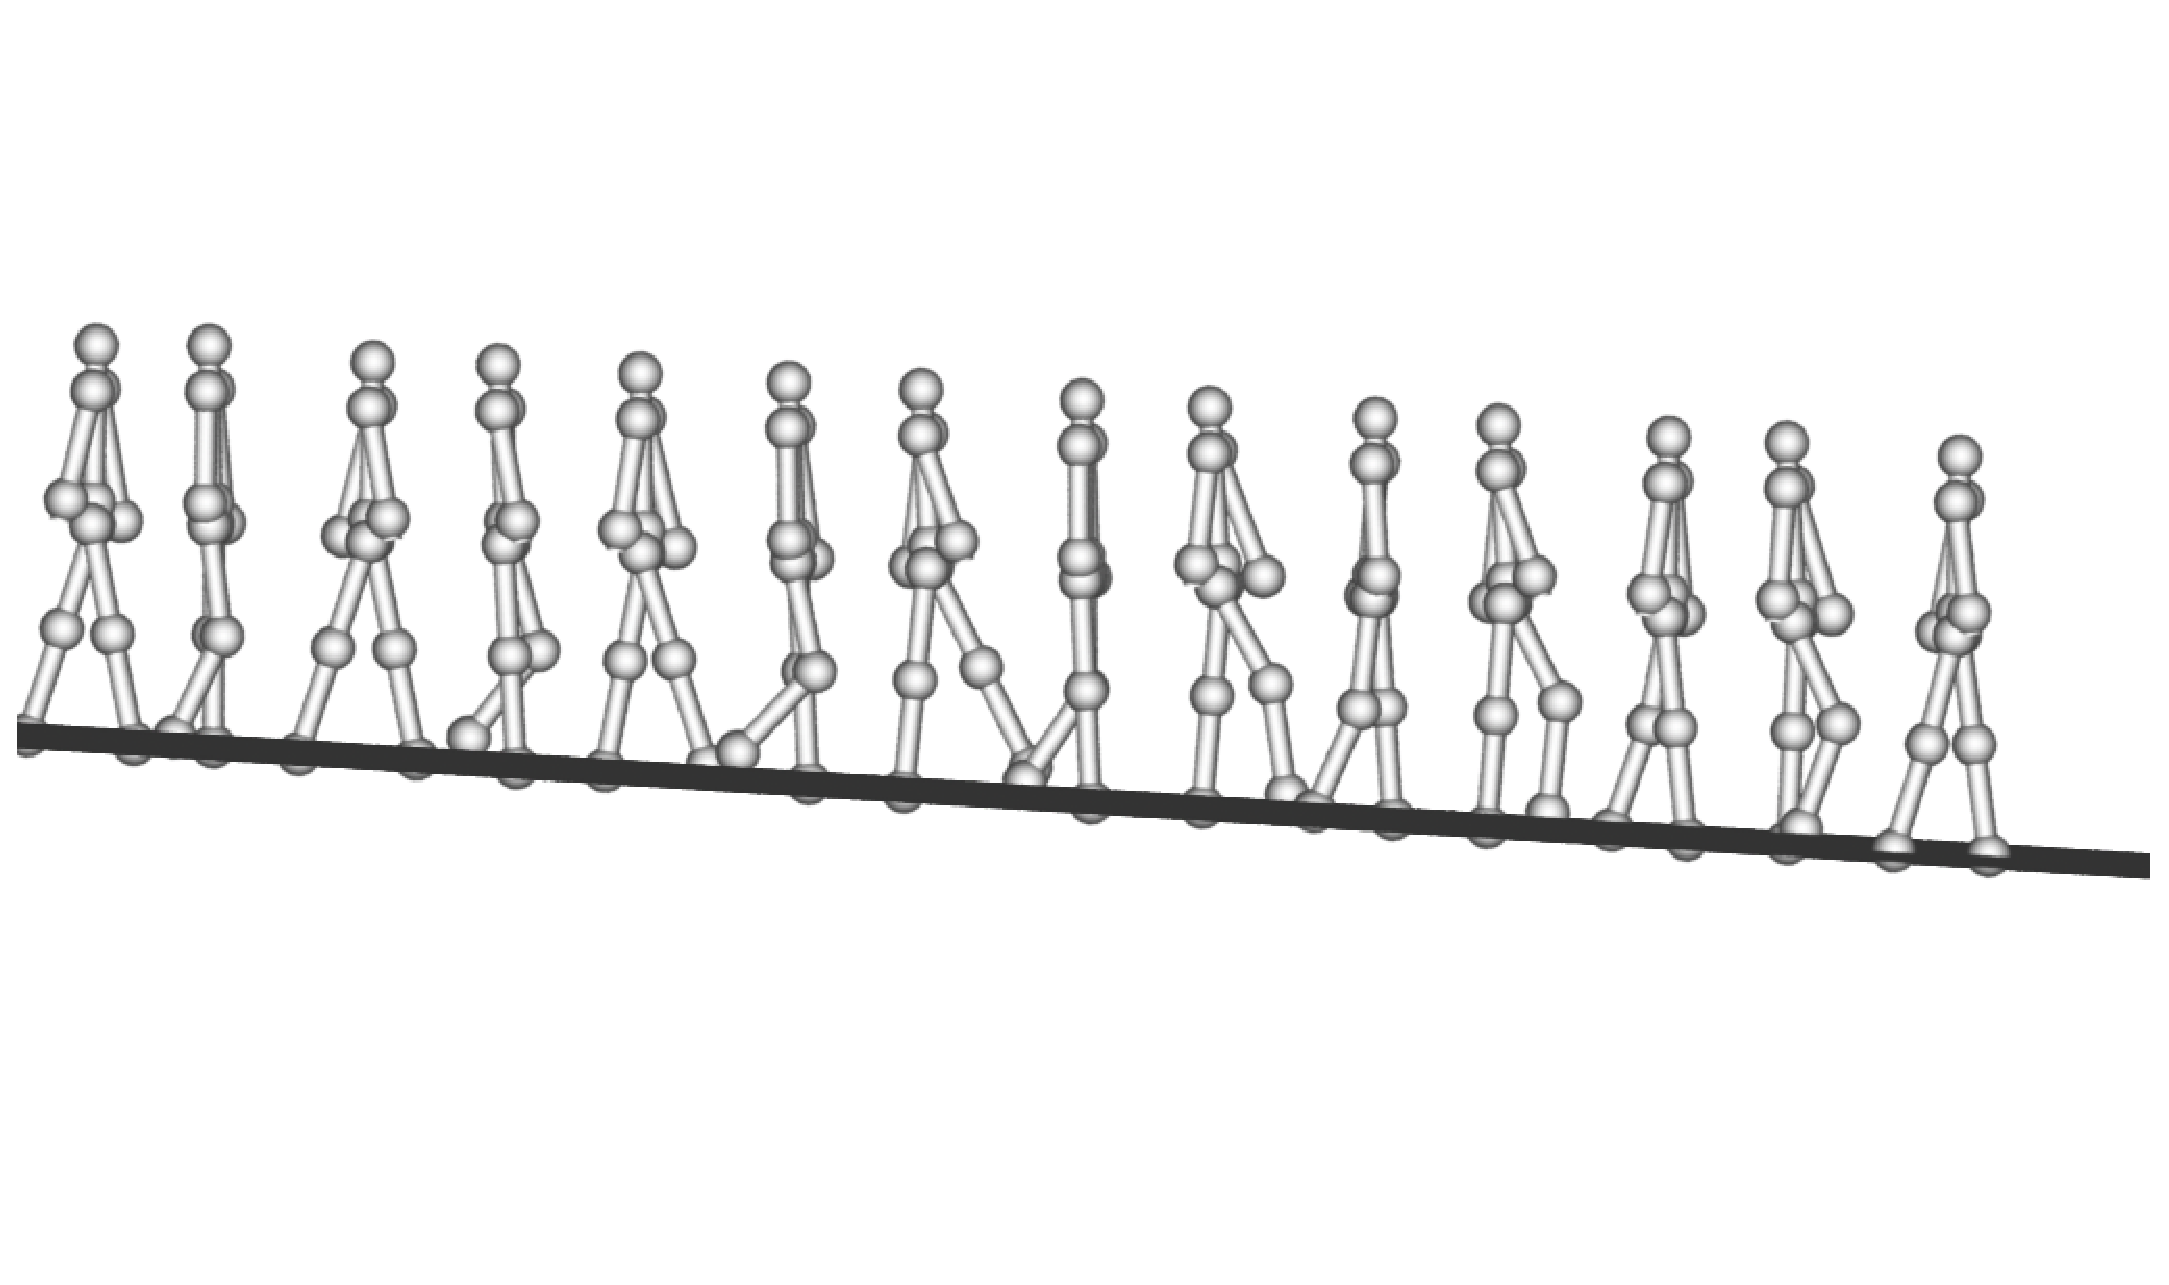
\includegraphics[width=0.7\textwidth]{BigStep}
    \caption{Big Initial Step Size}
    \label{fig:bigStepIni}
\end{center}
\end{figure}


\begin{figure}[!htbp]
  \begin{center}
      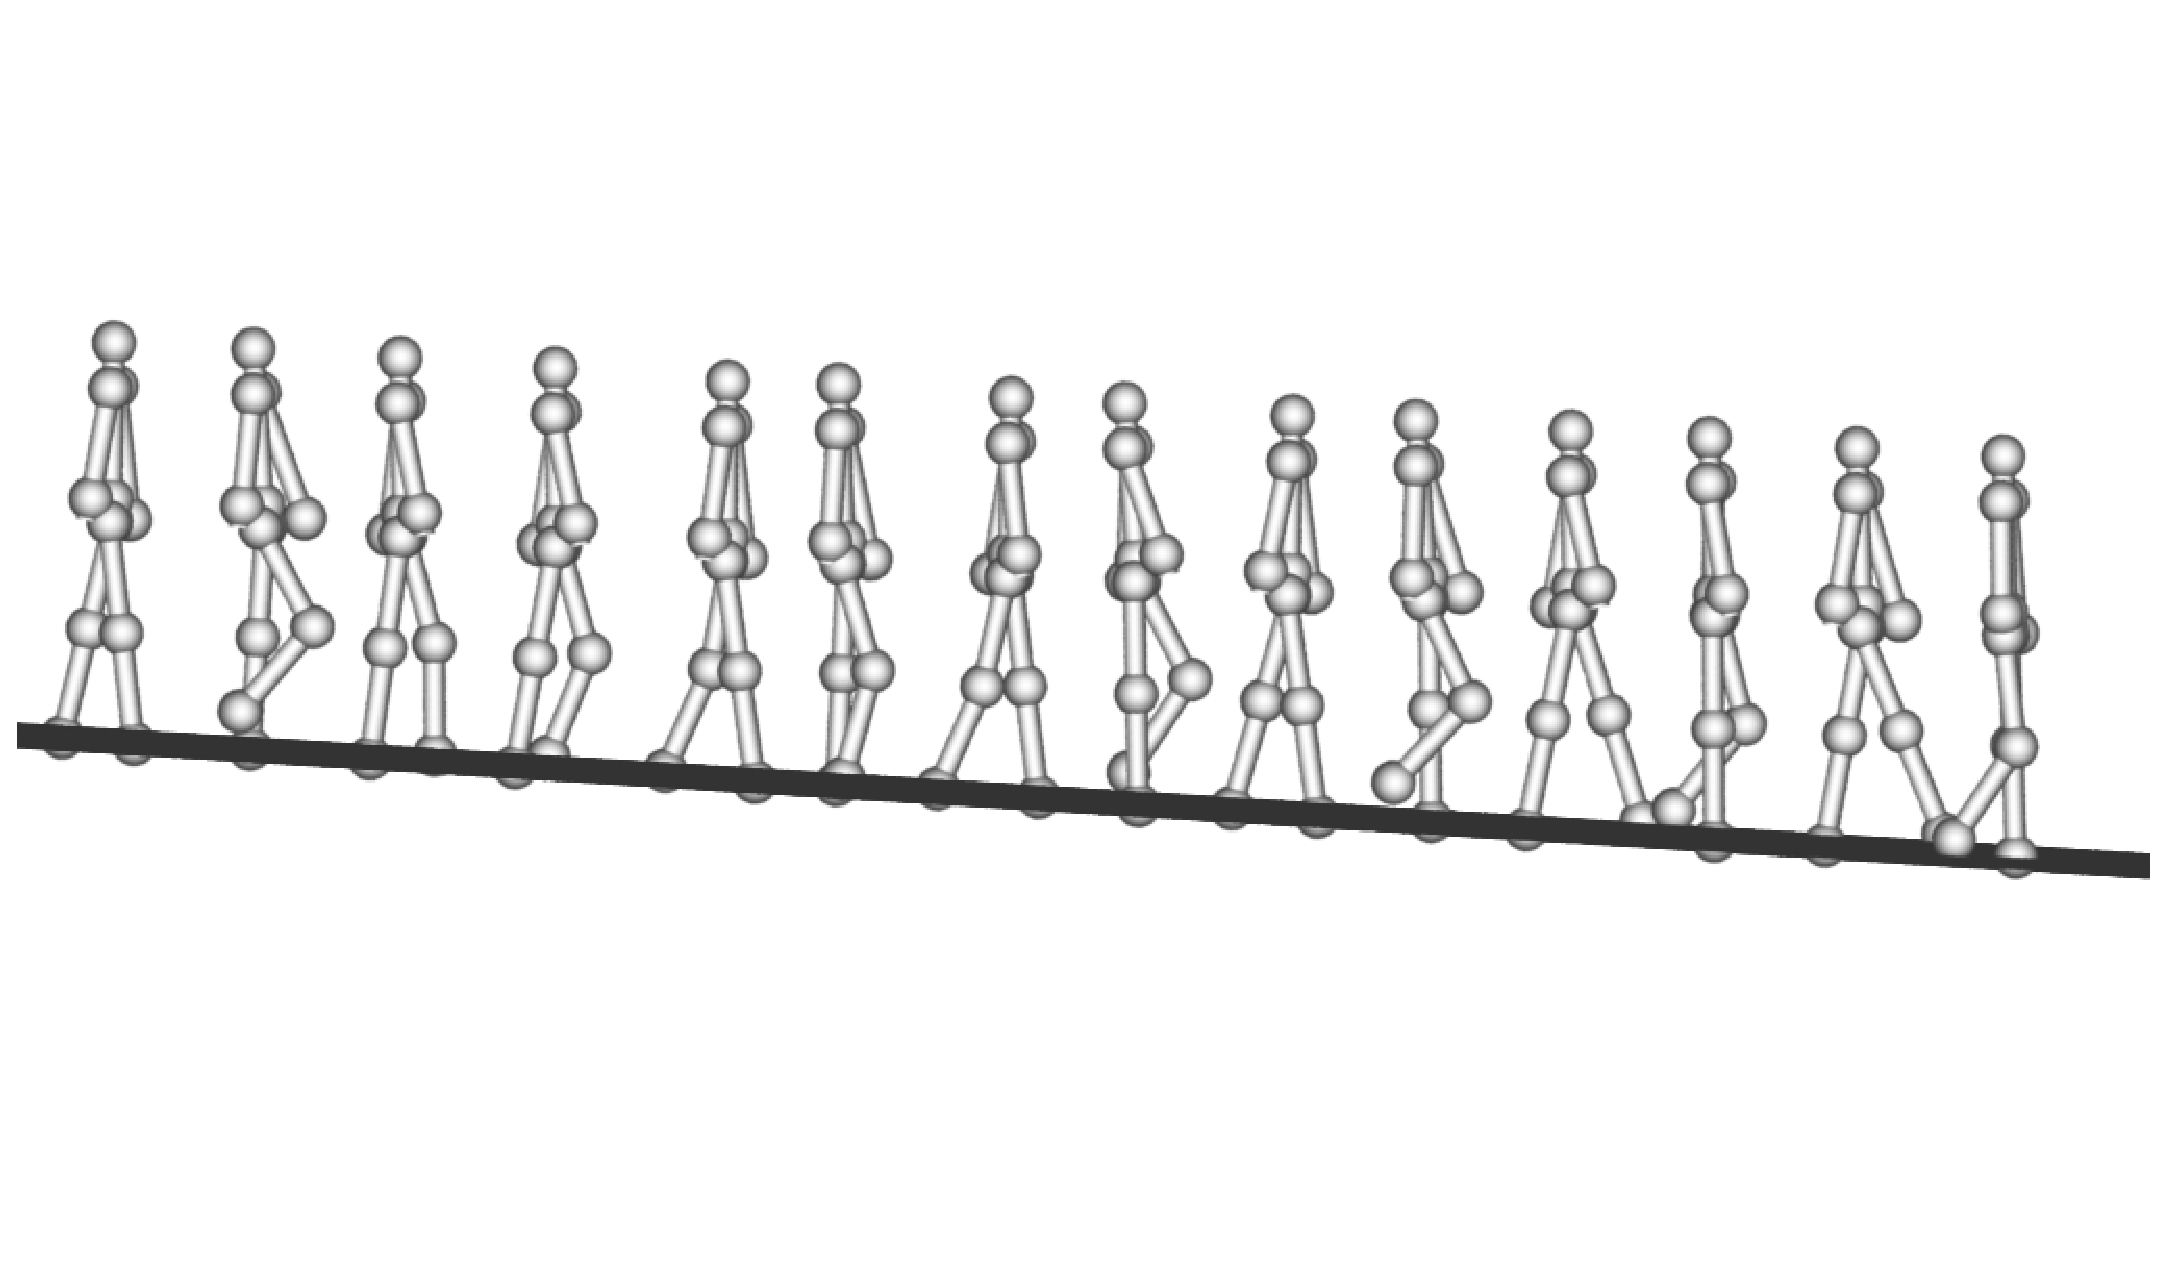
\includegraphics[width=0.7\textwidth]{smallStep}
    \caption{Small Initial Step Size}
    \label{fig:smallStepini}
\end{center}
\end{figure}


\begin{figure}[!htbp]
  \begin{center}
      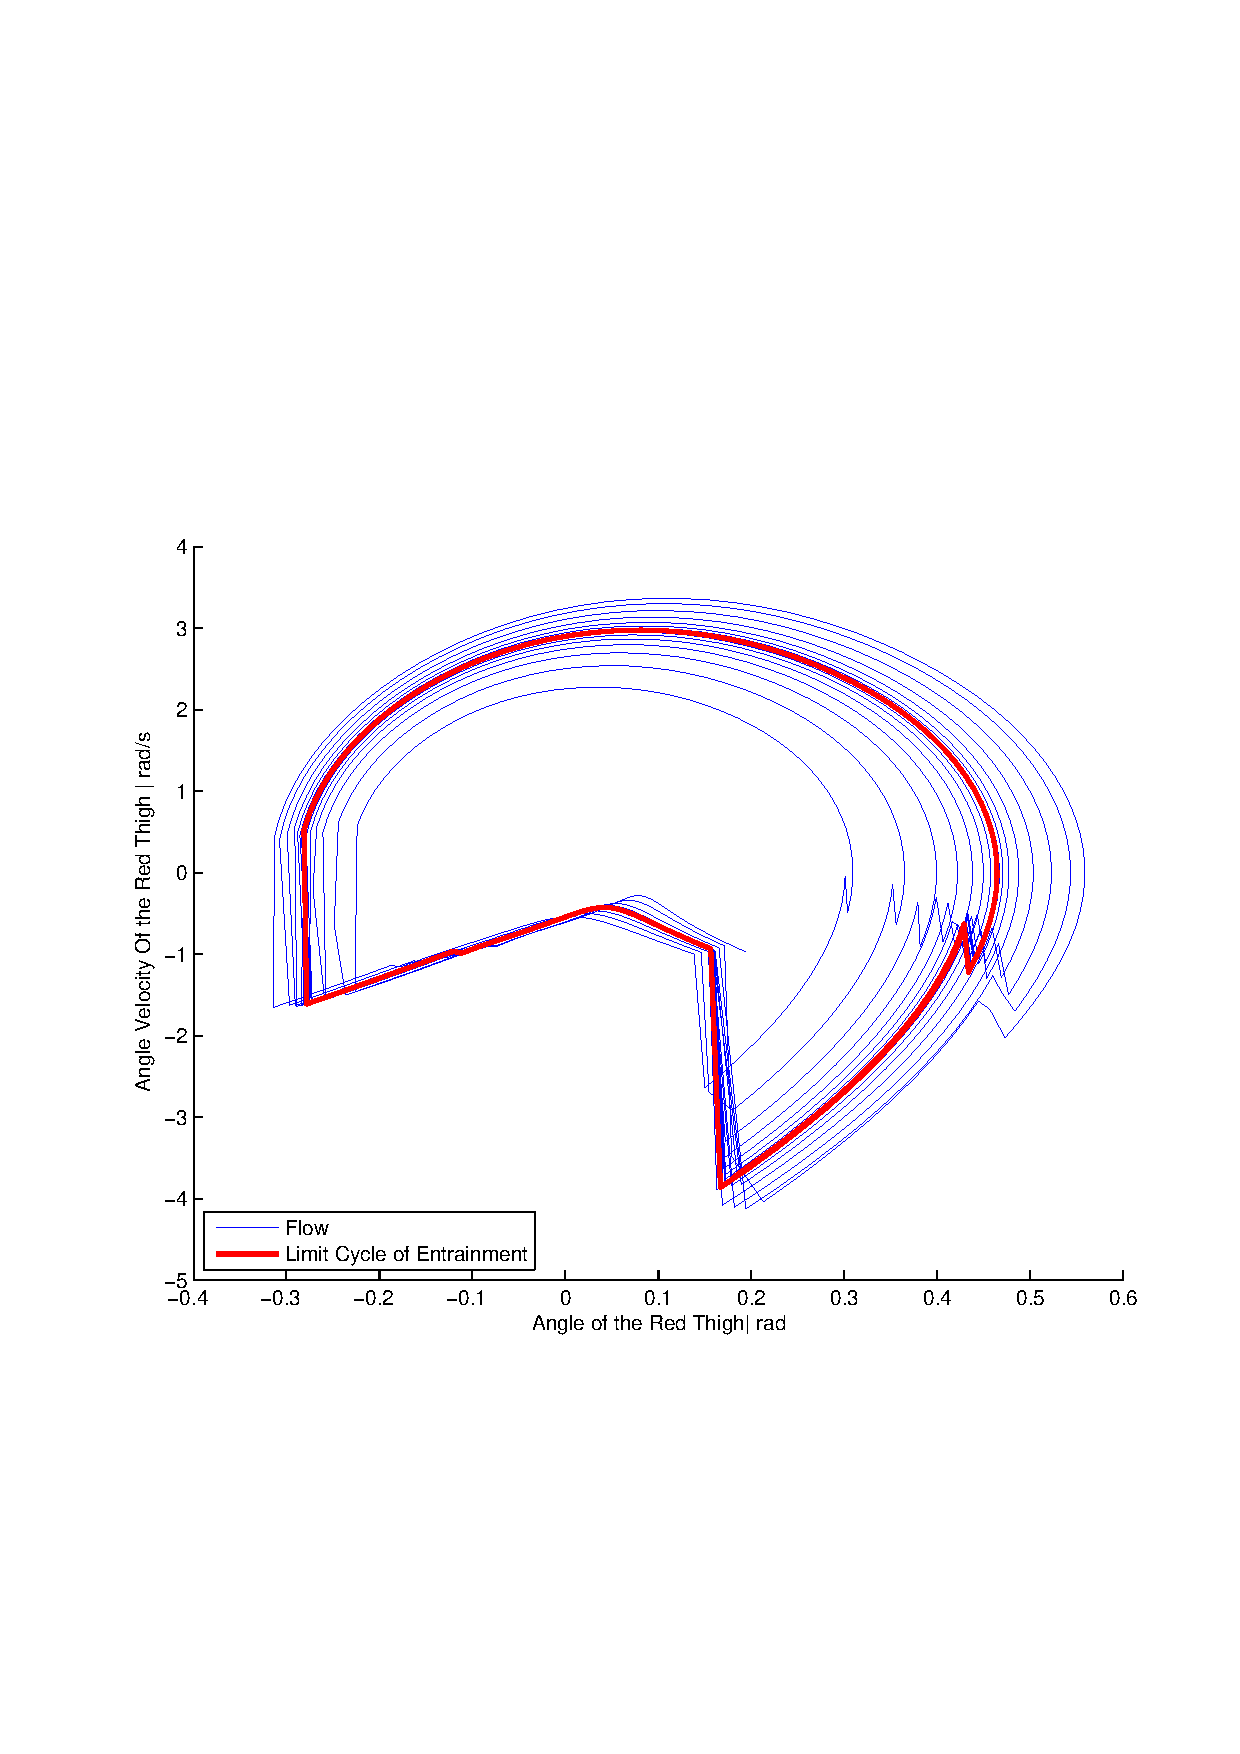
\includegraphics[width=0.7\textwidth]{BigStepPhasePlot}
    \caption{Big Initial Step Initial Phase Plot}
    \label{fig:bigstepiniGaitPlot}
\end{center}
\end{figure}


\begin{figure}[!htbp]
  \begin{center}
      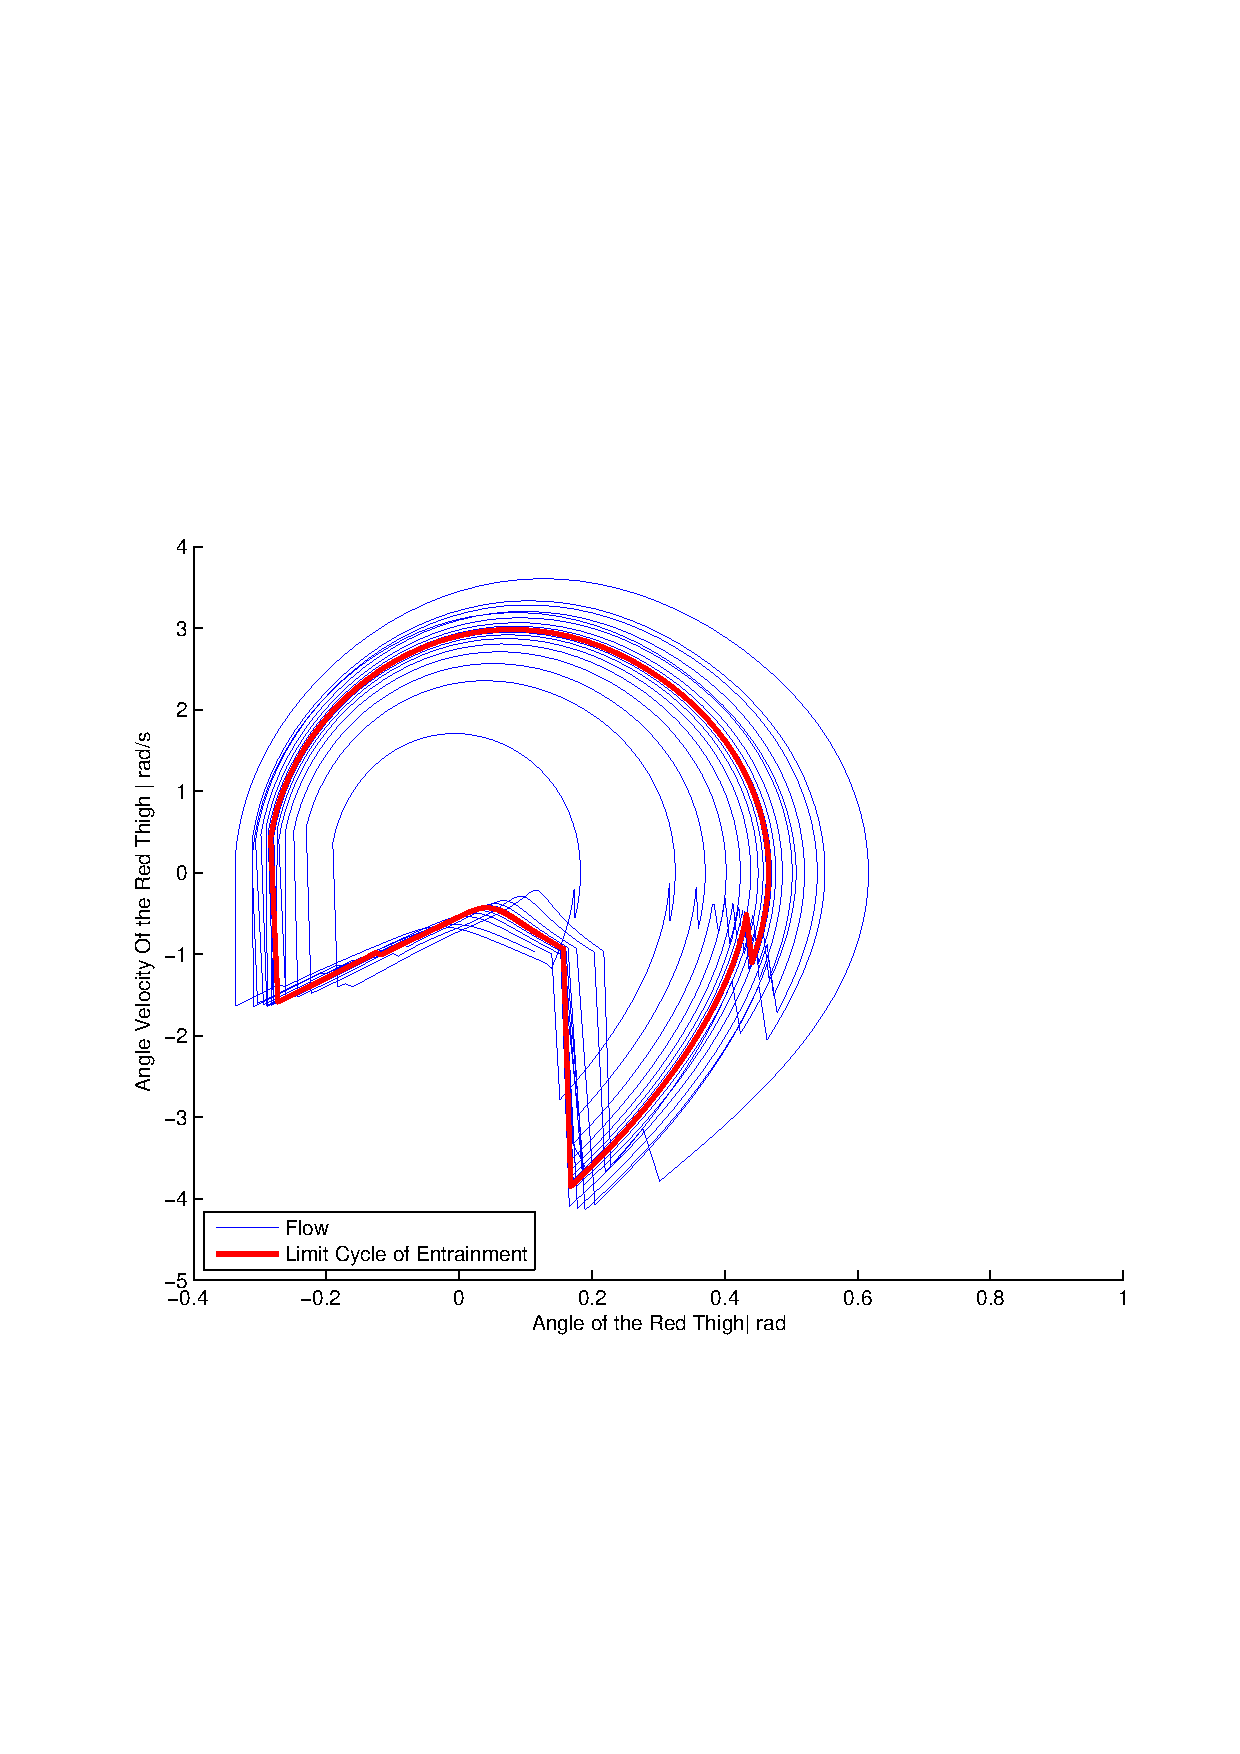
\includegraphics[width=0.7\textwidth]{SmallStepPhasePlot}
    \caption{The Small Initial Step Gait Phase Plot}
    \label{fig:smallstepiniPhasePlot}
\end{center}
\end{figure}

The entrainment of \cpg\  greatly enlarges the basin of attraction.
If the walker starts with very different postures, the character will return to normal walk.





\subsection{Walking Re-targeting}
Transferring the gait of one character to another is a challenging job.
\moit\ theory provides a method for physics based motion re-targeting.
\cpg\ will maintain the topology of the dynamics.
When the dynamic parameters are changed, the topological conjugacy will result in a varied motion.

The passive walker has many parameters, like mass and leg length.
Different parameters will result in a different dynamics systems.
But all these dynamic systems  share the same topology.
There is a limit cycle and the characters are capable of periodic gaits.
Some interesting gaits are shown and discussed below in this section.

If all the parameters are scaled  uniformly, the gait will remain the same, only the velocity will be changed.
To demonstrate different gaits, the parameters are modified relatively. 
The motion variation is generated by adjusting the mass ratio and mass distribution ratio, the total mass and total leg length of all examples are kept the same.



\subsubsection*{Mass Distribution Ratio}
When the total mass is maintained,
Mass Distribution Ratio is defined as the hip mass over leg mass. 
\[
\alpha_m=\frac{m_h}{m_s}
\]
where $m_h$ is the mass of the hip and $m_t$ is mass of the thigh.
The mass ratios of shank and thigh is kept unchanged.

Different $\alpha_m$ will result in different gaits.
Bigger $\alpha_m$ result in gaits to that  look burdened.
The different limit cycles are shown in Figure ~\ref{fig:differentmh}.
\begin{figure}[!htbp]
  \begin{center}
     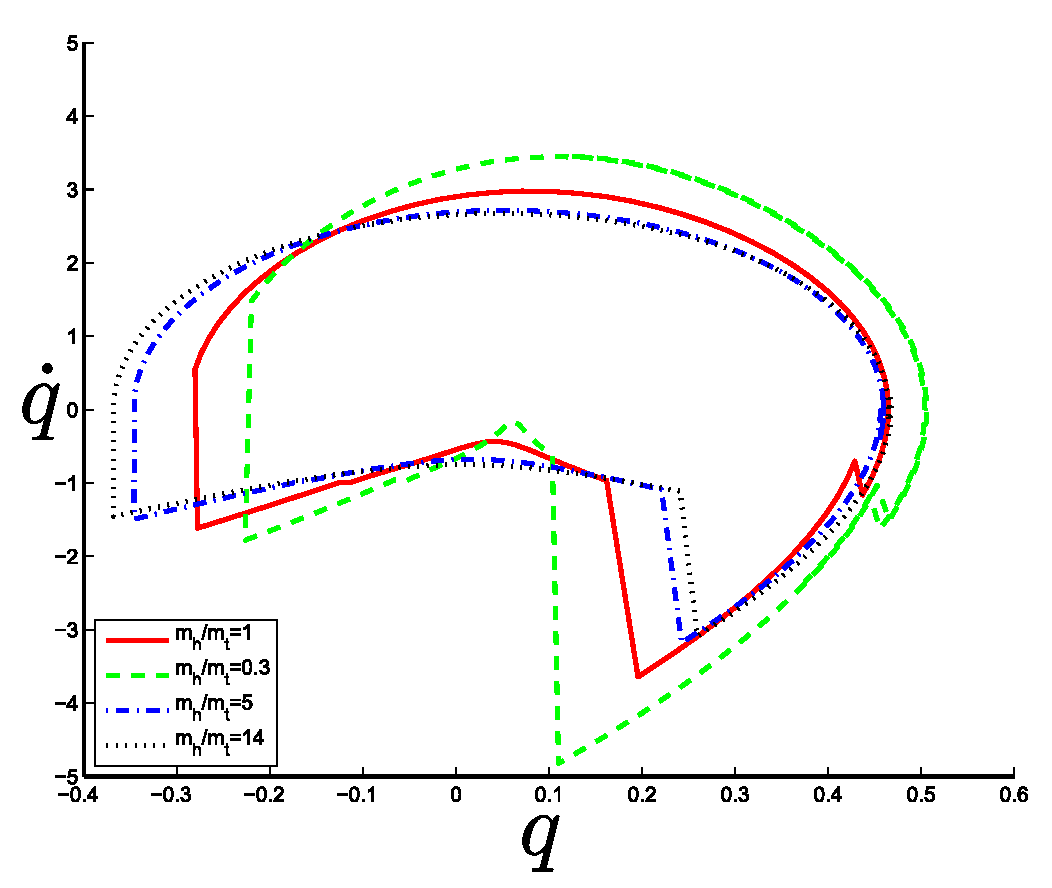
\includegraphics[width=0.7\textwidth]{MassDistributionEffectsOnLimitCircle}
    \caption{Different Gait Resulting from the Different Mass Ratio}
    \label{fig:differentmh}
\end{center}
\end{figure}

For bigger $\alpha_m$, the walker will walk with a  bigger step but a slow speed($\qd$ is lower).
In addition, the character tends to fall backward.
For smaller $\alpha_m$, character will walk more quickly($\qd$ is bigger) and it tends to lean forward.
This may imply about the upper body motion.
Usually, when we carry something heavier, we tend to bend upper body forward.

Different gaits are shown in Figure~\ref{fig:massh1}, Figure~\ref{fig:massh2} and Figure~\ref{fig:massh3}.
\begin{figure}[!htbp]
  \begin{center}
      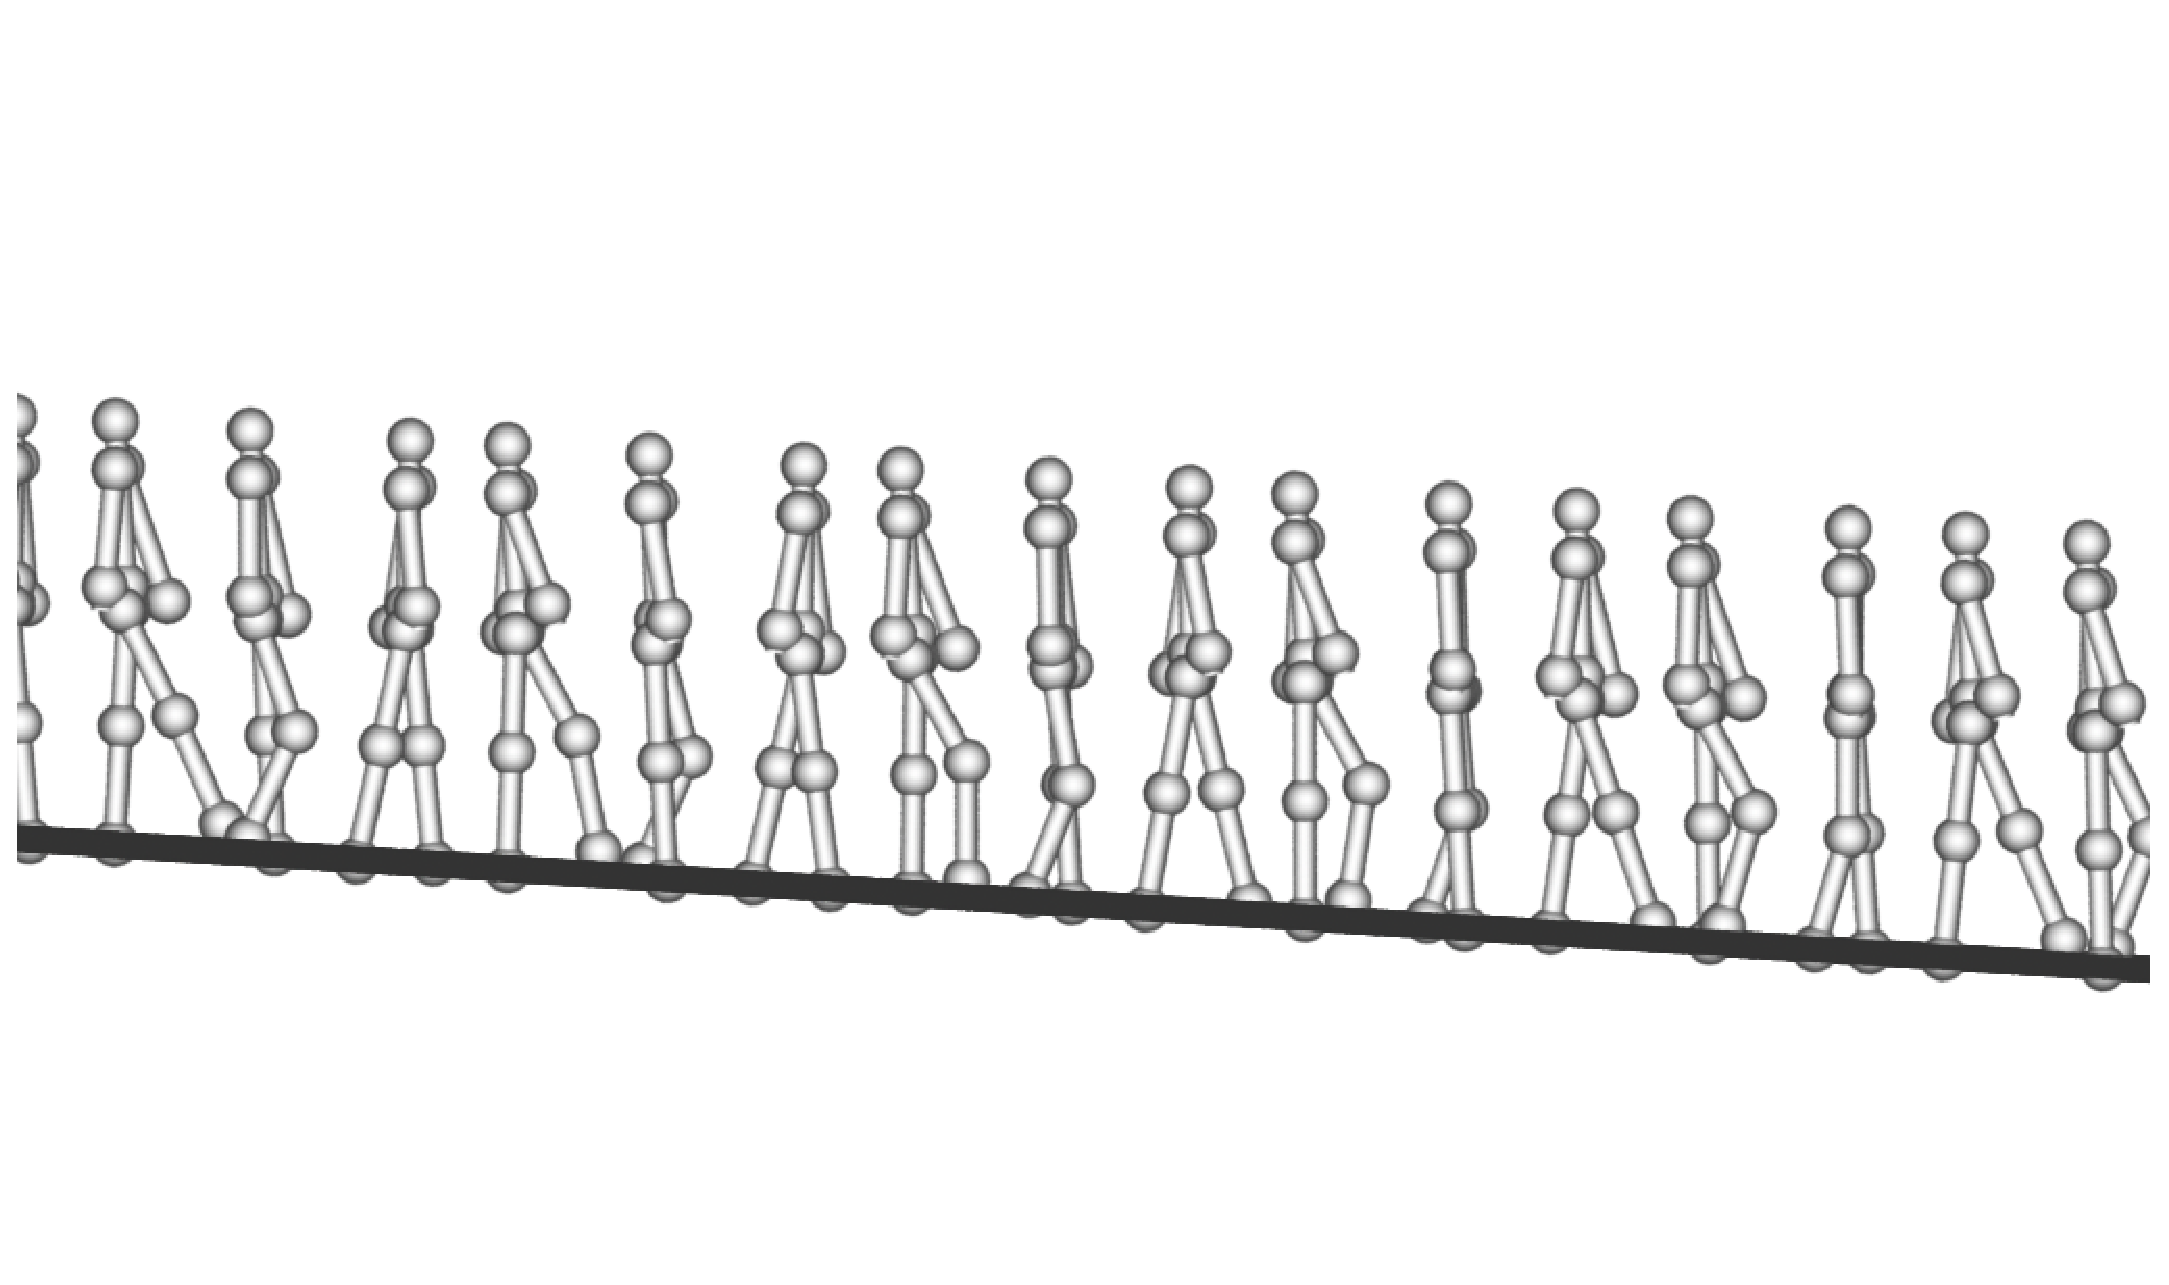
\includegraphics[width=0.7\textwidth]{mhms3}
    \caption{Gait with $\alpha_m=0.3$}
    \label{fig:massh1}
\end{center}
\end{figure}

\begin{figure}[!htbp]
  \begin{center}
      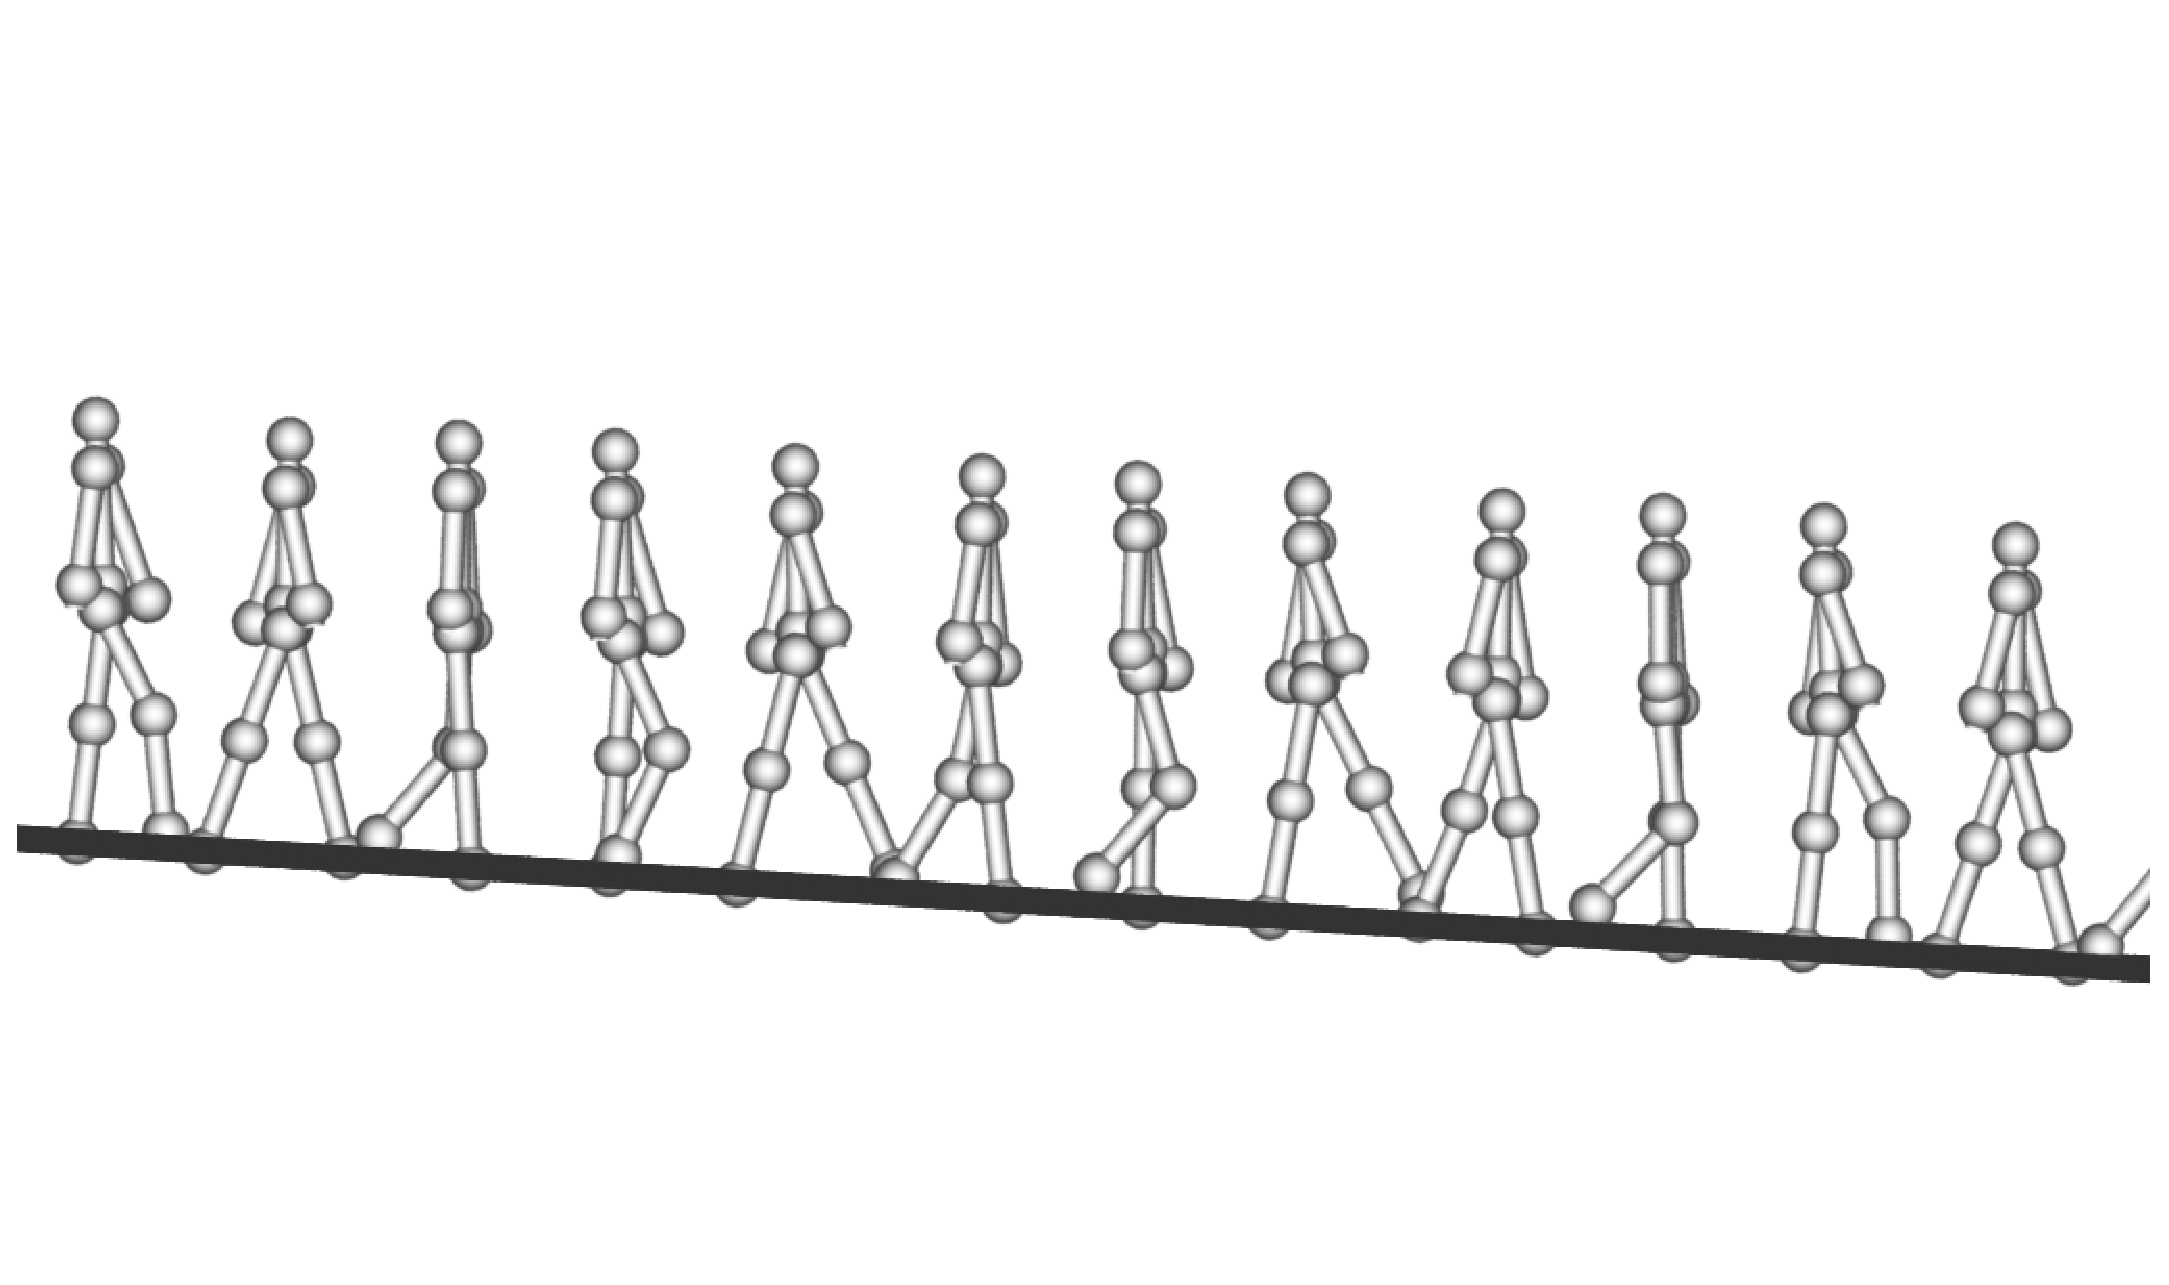
\includegraphics[width=0.7\textwidth]{mhms50}
    \caption{Gait with $\alpha_m=5$}
    \label{fig:massh2}
\end{center}
\end{figure}

\begin{figure}[!htbp]
  \begin{center}
      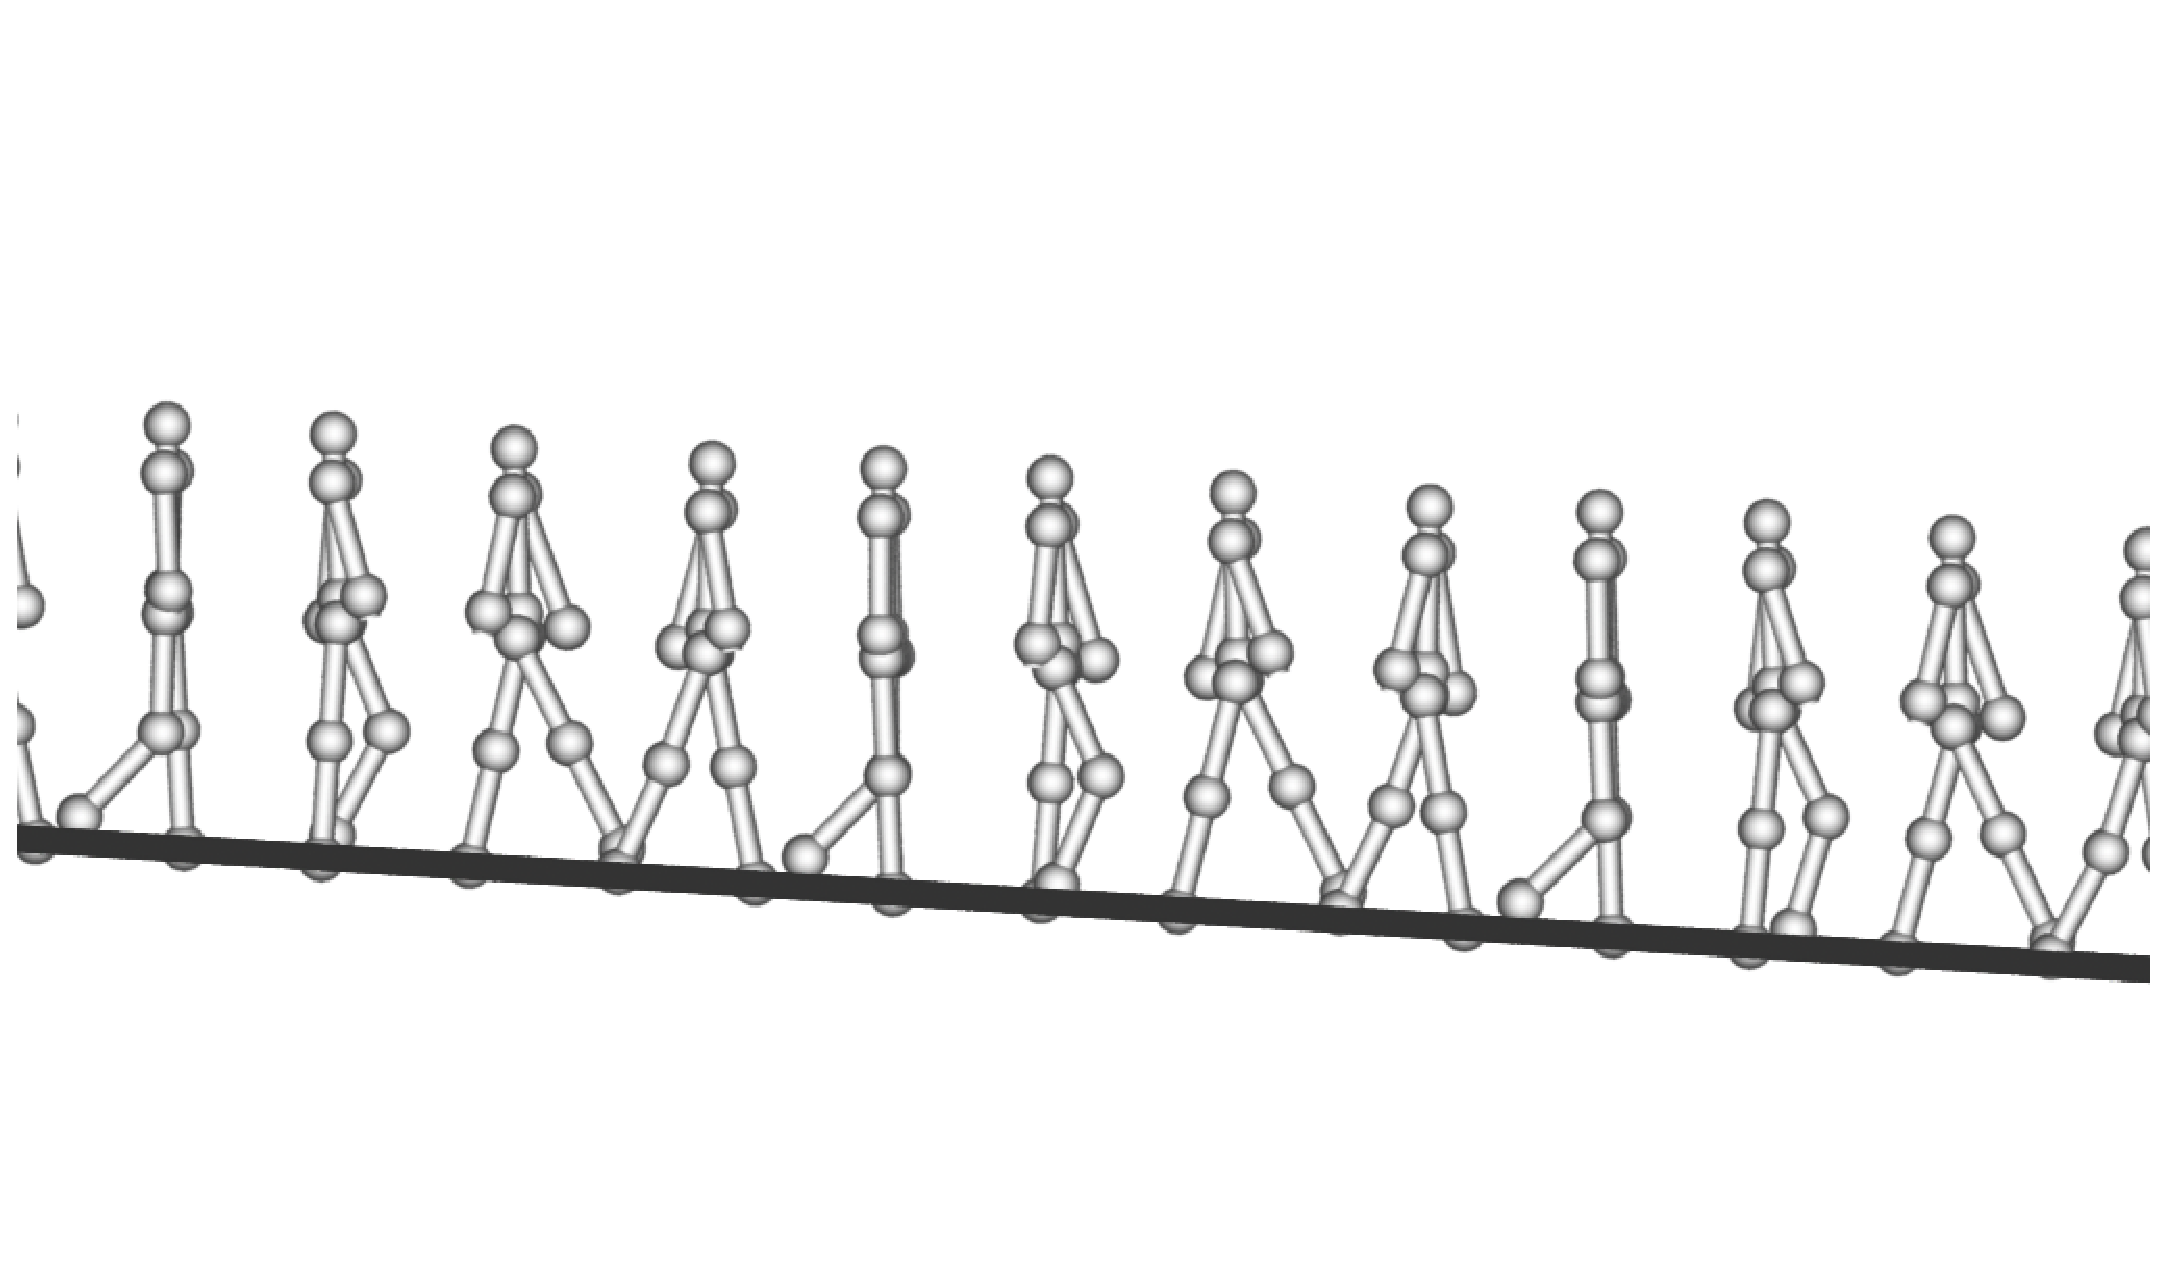
\includegraphics[width=0.7\textwidth]{mhms140}
    \caption{Gait with $\alpha_m=14$}
    \label{fig:massh3}
\end{center}
\end{figure}



\subsubsection*{Leg Length Distribution Ratio}
Except for the change of the ratio parameter  $\alpha_l=\frac{l_t}{l_s}$, the leg length is kept unchanged.
By changing $\alpha_l$ motion for different characters are generated.
This demonstrates the motion re-targeting results.


\begin{figure}[!htbp]
  \begin{center}
      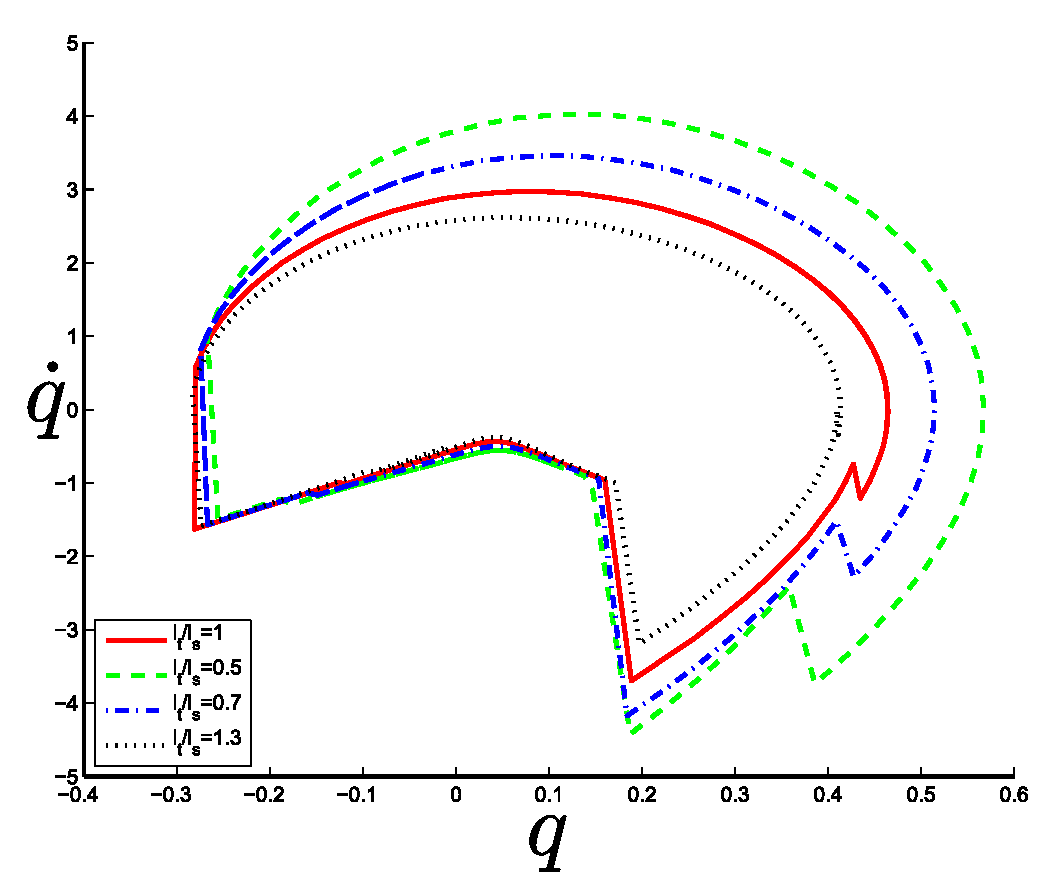
\includegraphics[width=0.7\textwidth]{LegLengthDistributionEffectsOnLimitCircle}
    \caption{Different Gait Resulting from the Different Mass Ratio}
    \label{fig:differentlr}
\end{center}
\end{figure}

The limit cycle in Figure~\ref{fig:differentlr} implies something important about leg length in walking.
Basically, the  motions of the supporting leg and the step size are almost kept the same, while different leg length rations will result in different swing motions.
The longer the shank, thigh has to swing quickly and with a bigger amplitude.
There are also bigger impulses during the strike phase. 
For both the knee and heel strike, larger impulse is generated.
This result may indicate the effects of high heel shoes for walking.

Figure~\ref{fig:lr1}, Figure~\ref{fig:lr2} and Figure~\ref{fig:lr3} show the different gaits.
\begin{figure}[!htbp]
  \begin{center}
      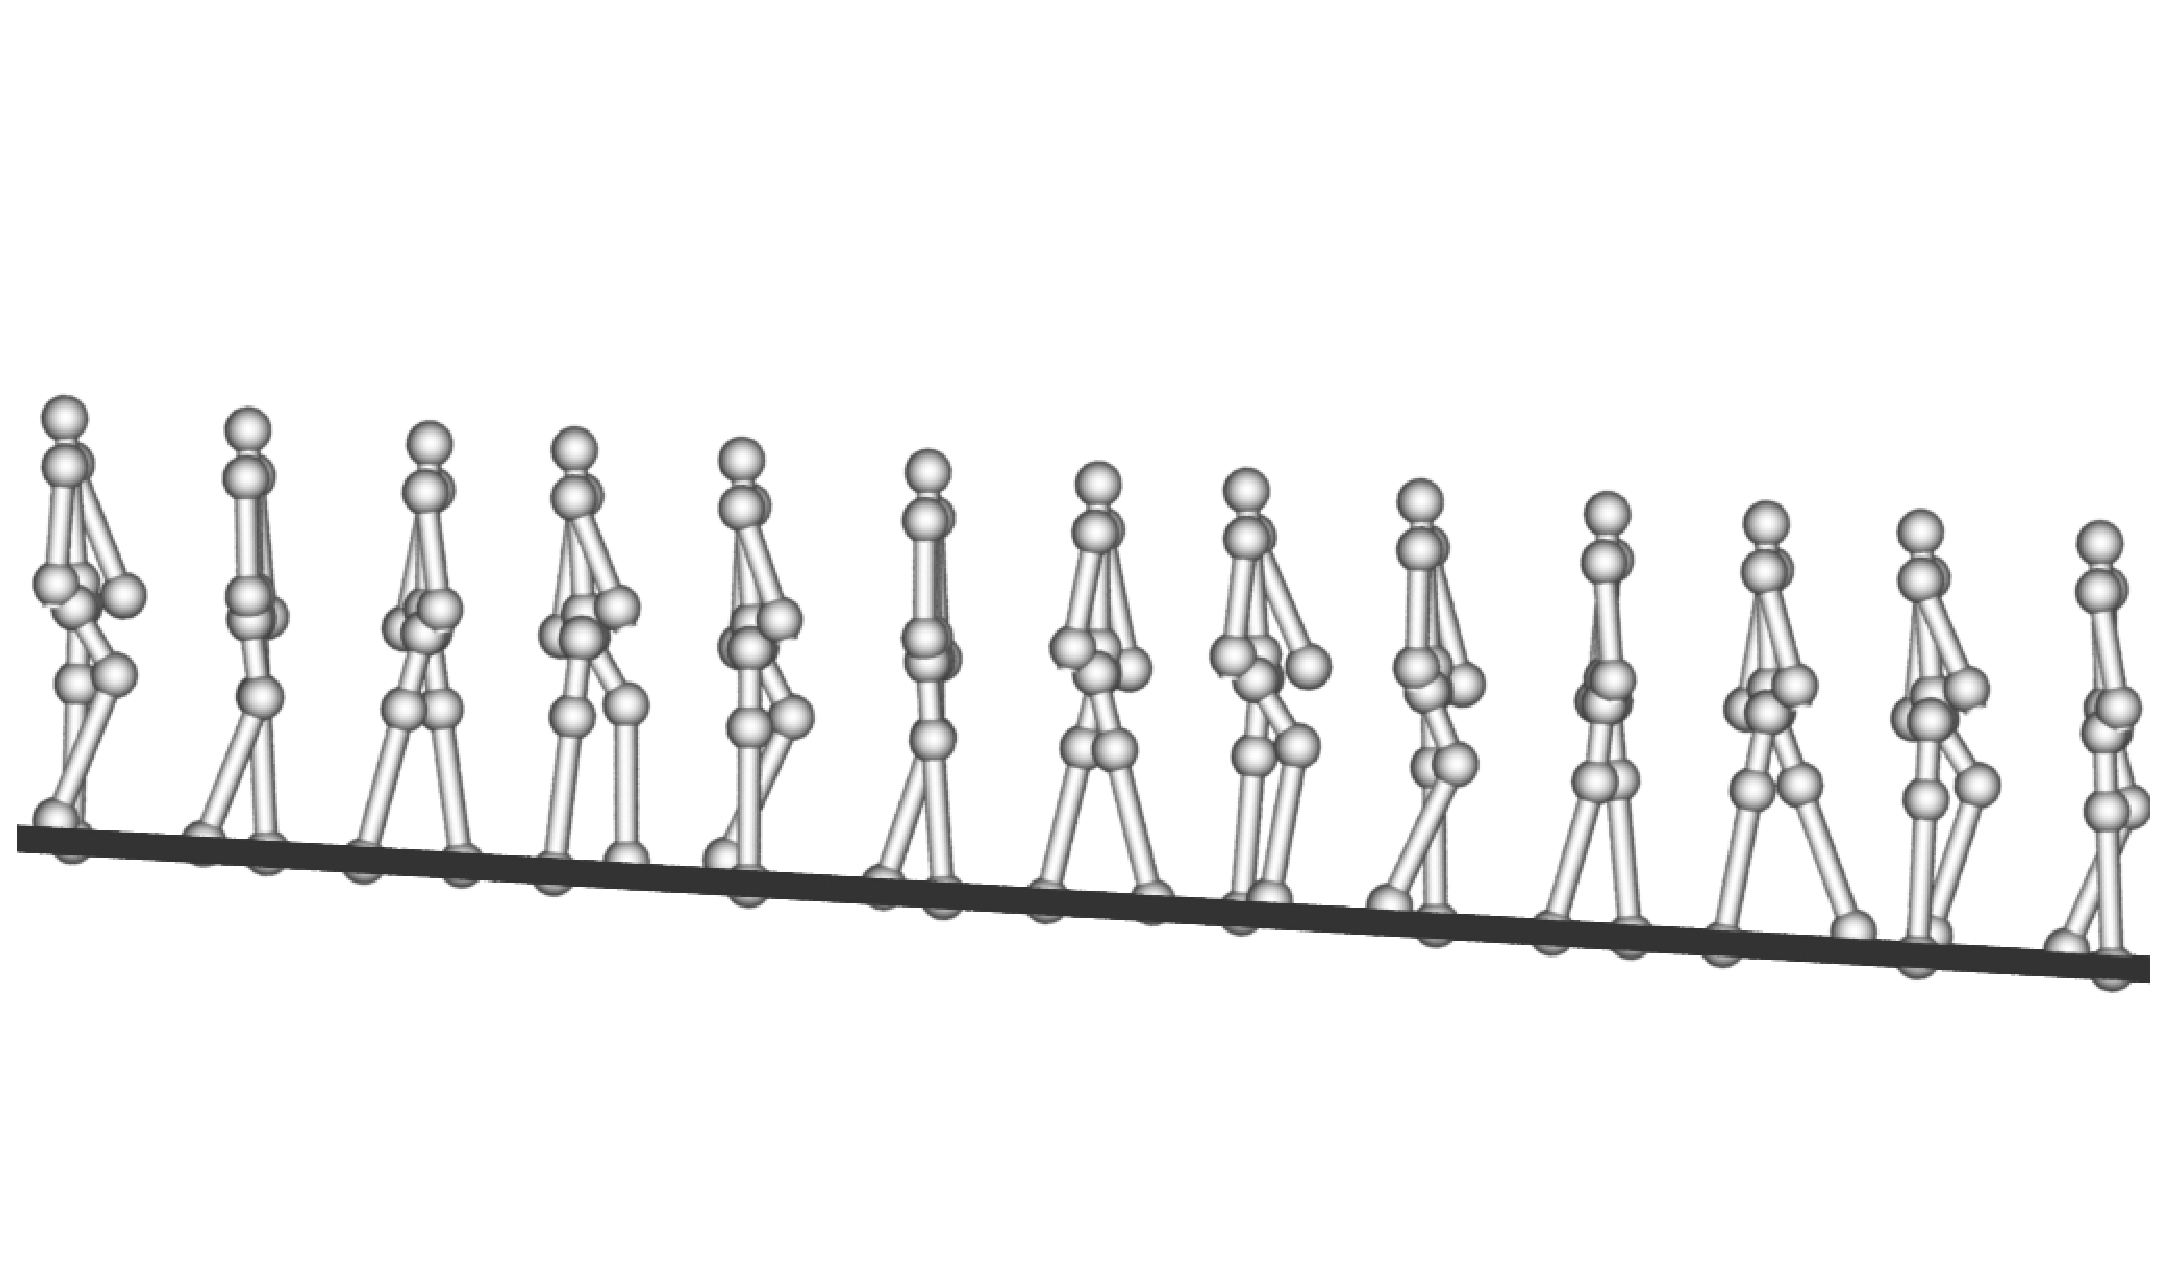
\includegraphics[width=0.7\textwidth]{LTLS5}
    \caption{gait of $\alpha_l=0.5$}
    \label{fig:lr1}
\end{center}
\end{figure}

\begin{figure}[!htbp]
  \begin{center}
      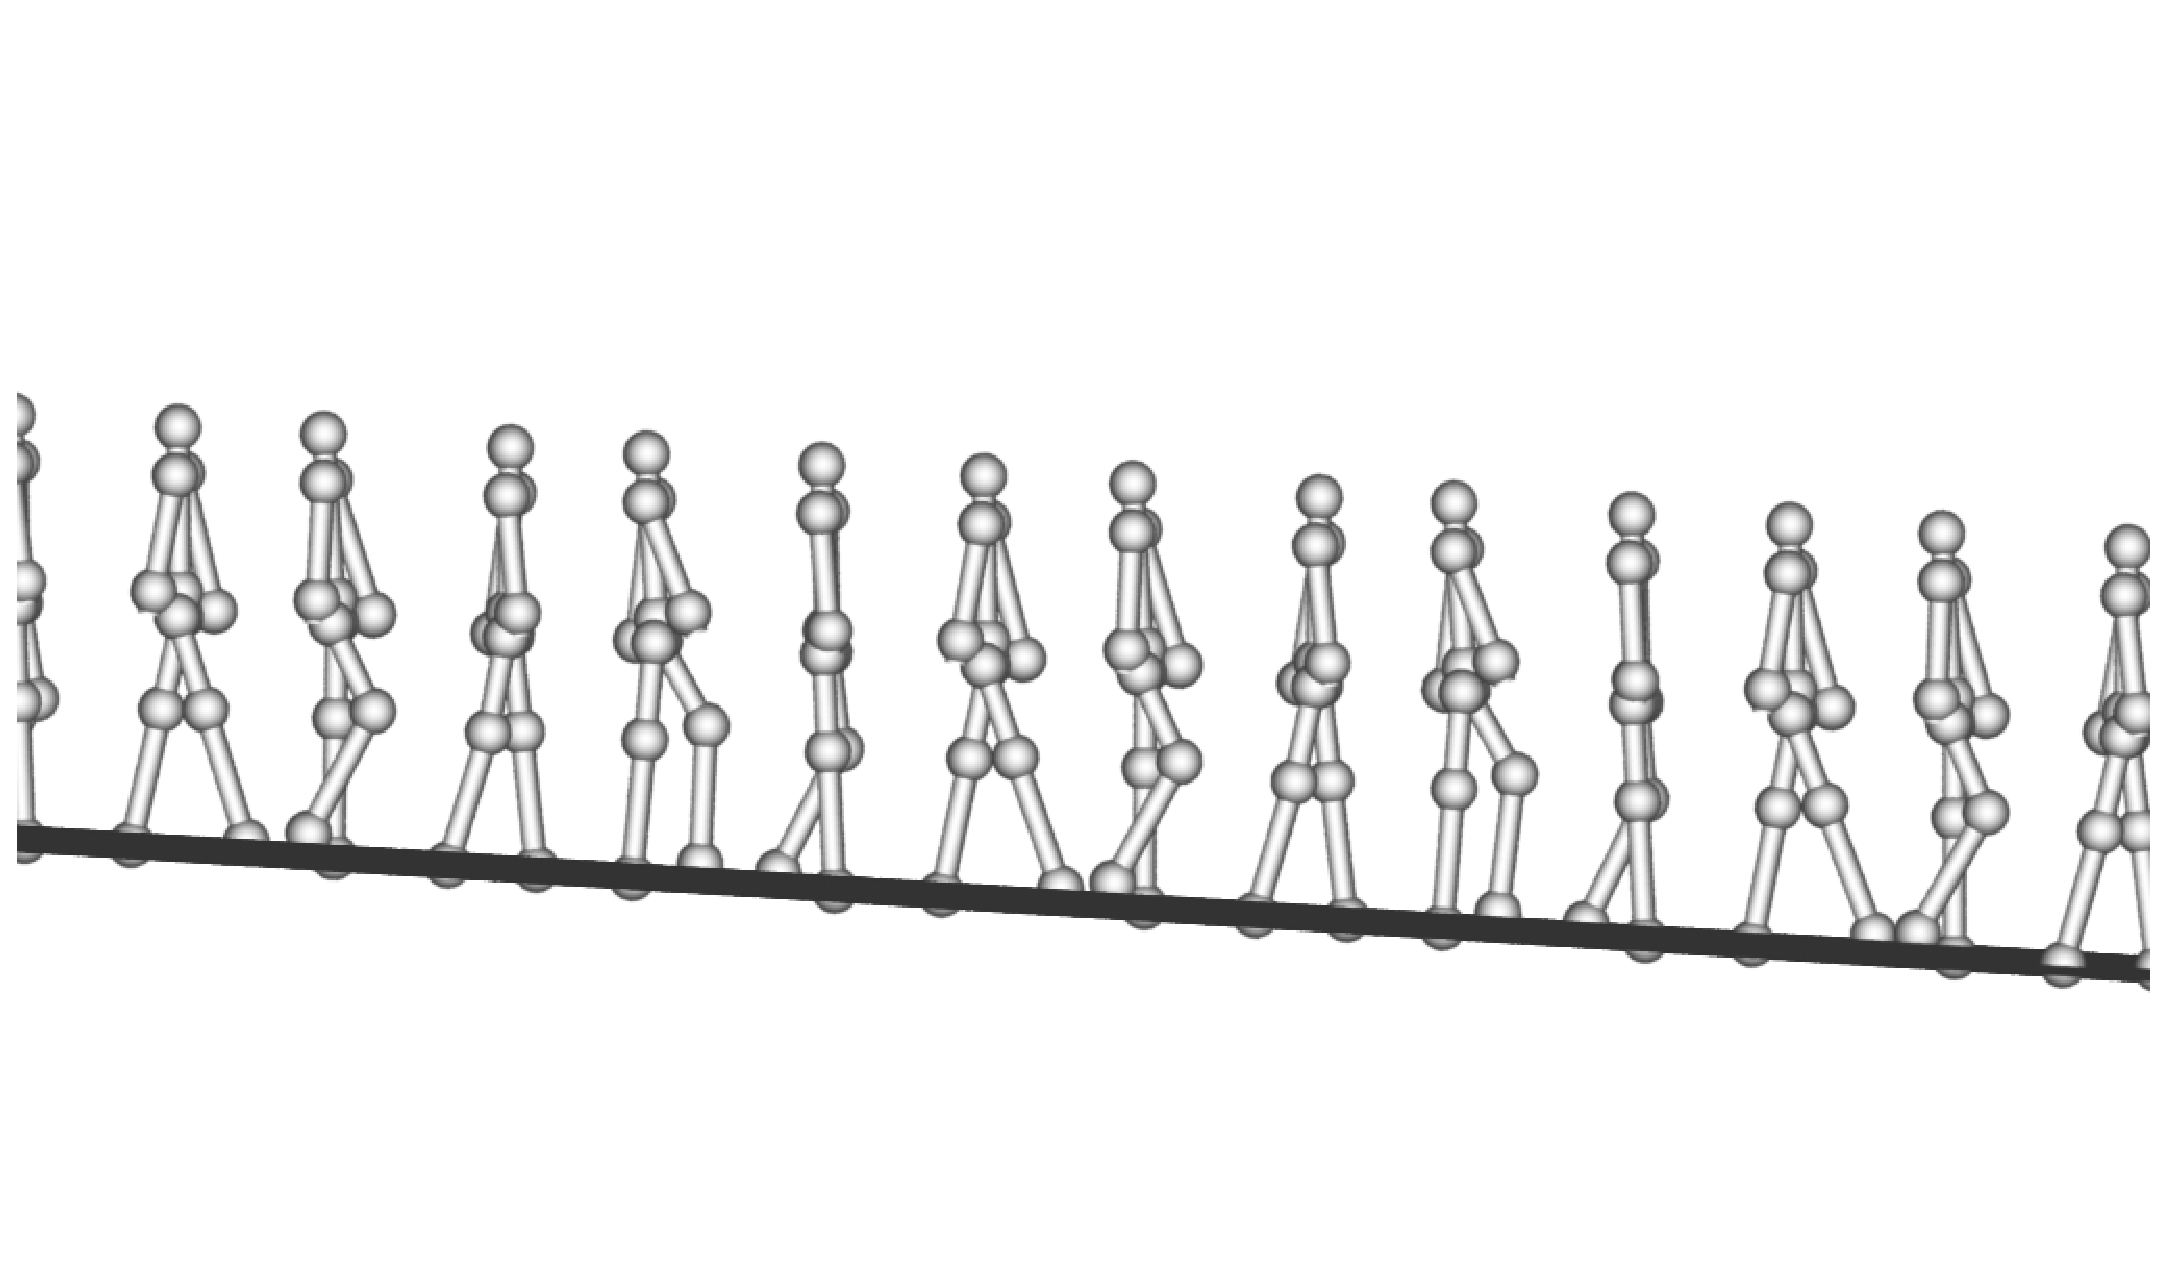
\includegraphics[width=0.7\textwidth]{LTLS7}
    \caption{gait of $\alpha_l=0.7$}
    \label{fig:lr2}
\end{center}
\end{figure}

\begin{figure}[!htbp]
  \begin{center}
      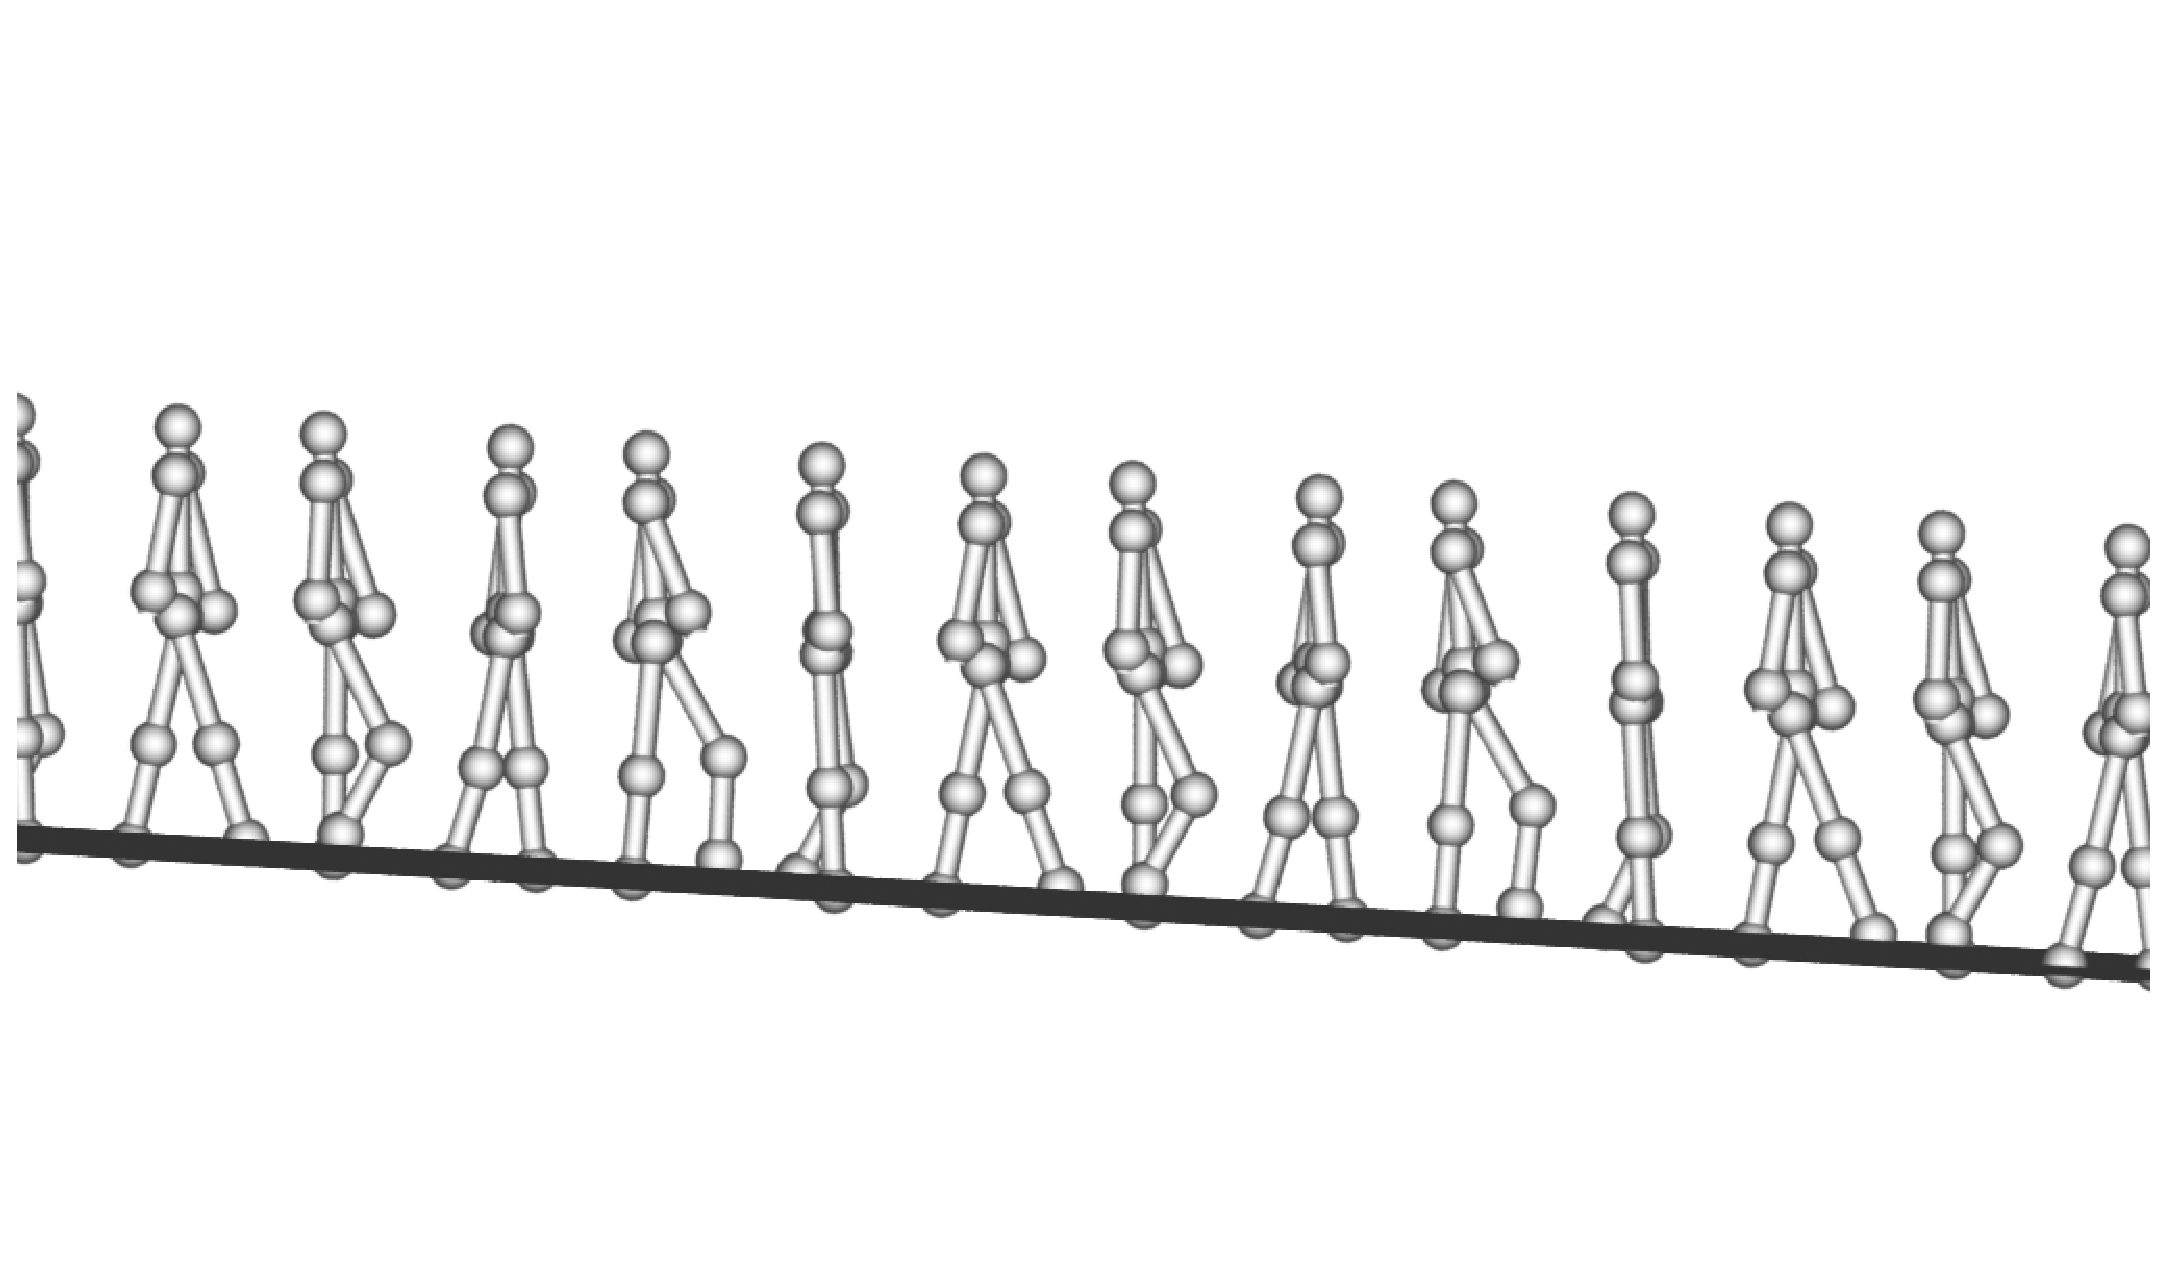
\includegraphics[width=0.7\textwidth]{LTLS13}
    \caption{gait of $\alpha_l=1.3$}
    \label{fig:lr3}
\end{center}
\end{figure}





\subsubsection*{Unbalanced Mass Ratio}
Also define the \emph{Unbalanced Mass Ration} 
\[
\alpha_b=\frac{\text{Left Leg Mass}}{\text{Right Leg Mass}}
\].


\begin{figure}[!htbp]
  \begin{center}
      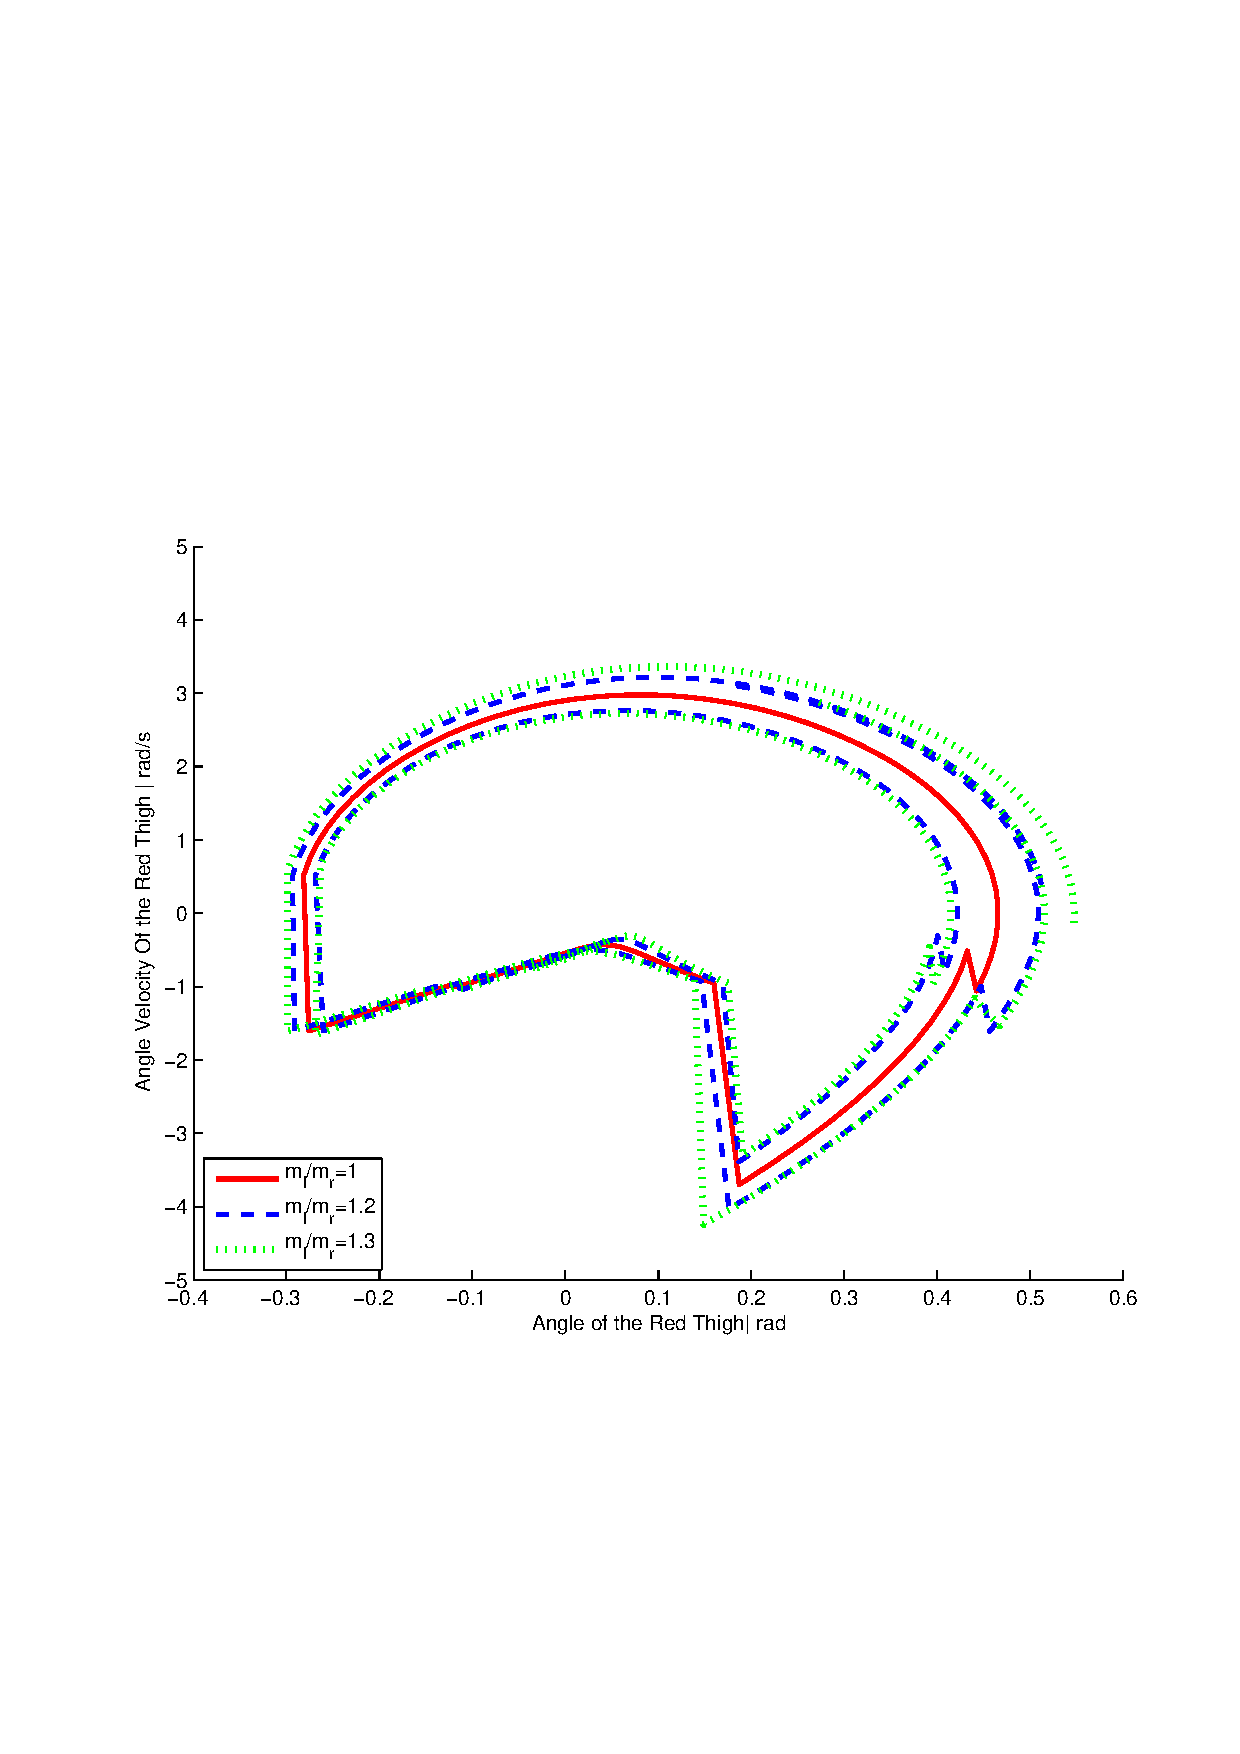
\includegraphics[width=0.7\textwidth]{DifferentLegMassLimitCircle}
    \caption{Different Leg Mass Stable Gaits}
    \label{fig:differentlr}
\end{center}
\end{figure}




\begin{figure}[!htbp]
  \begin{center}
      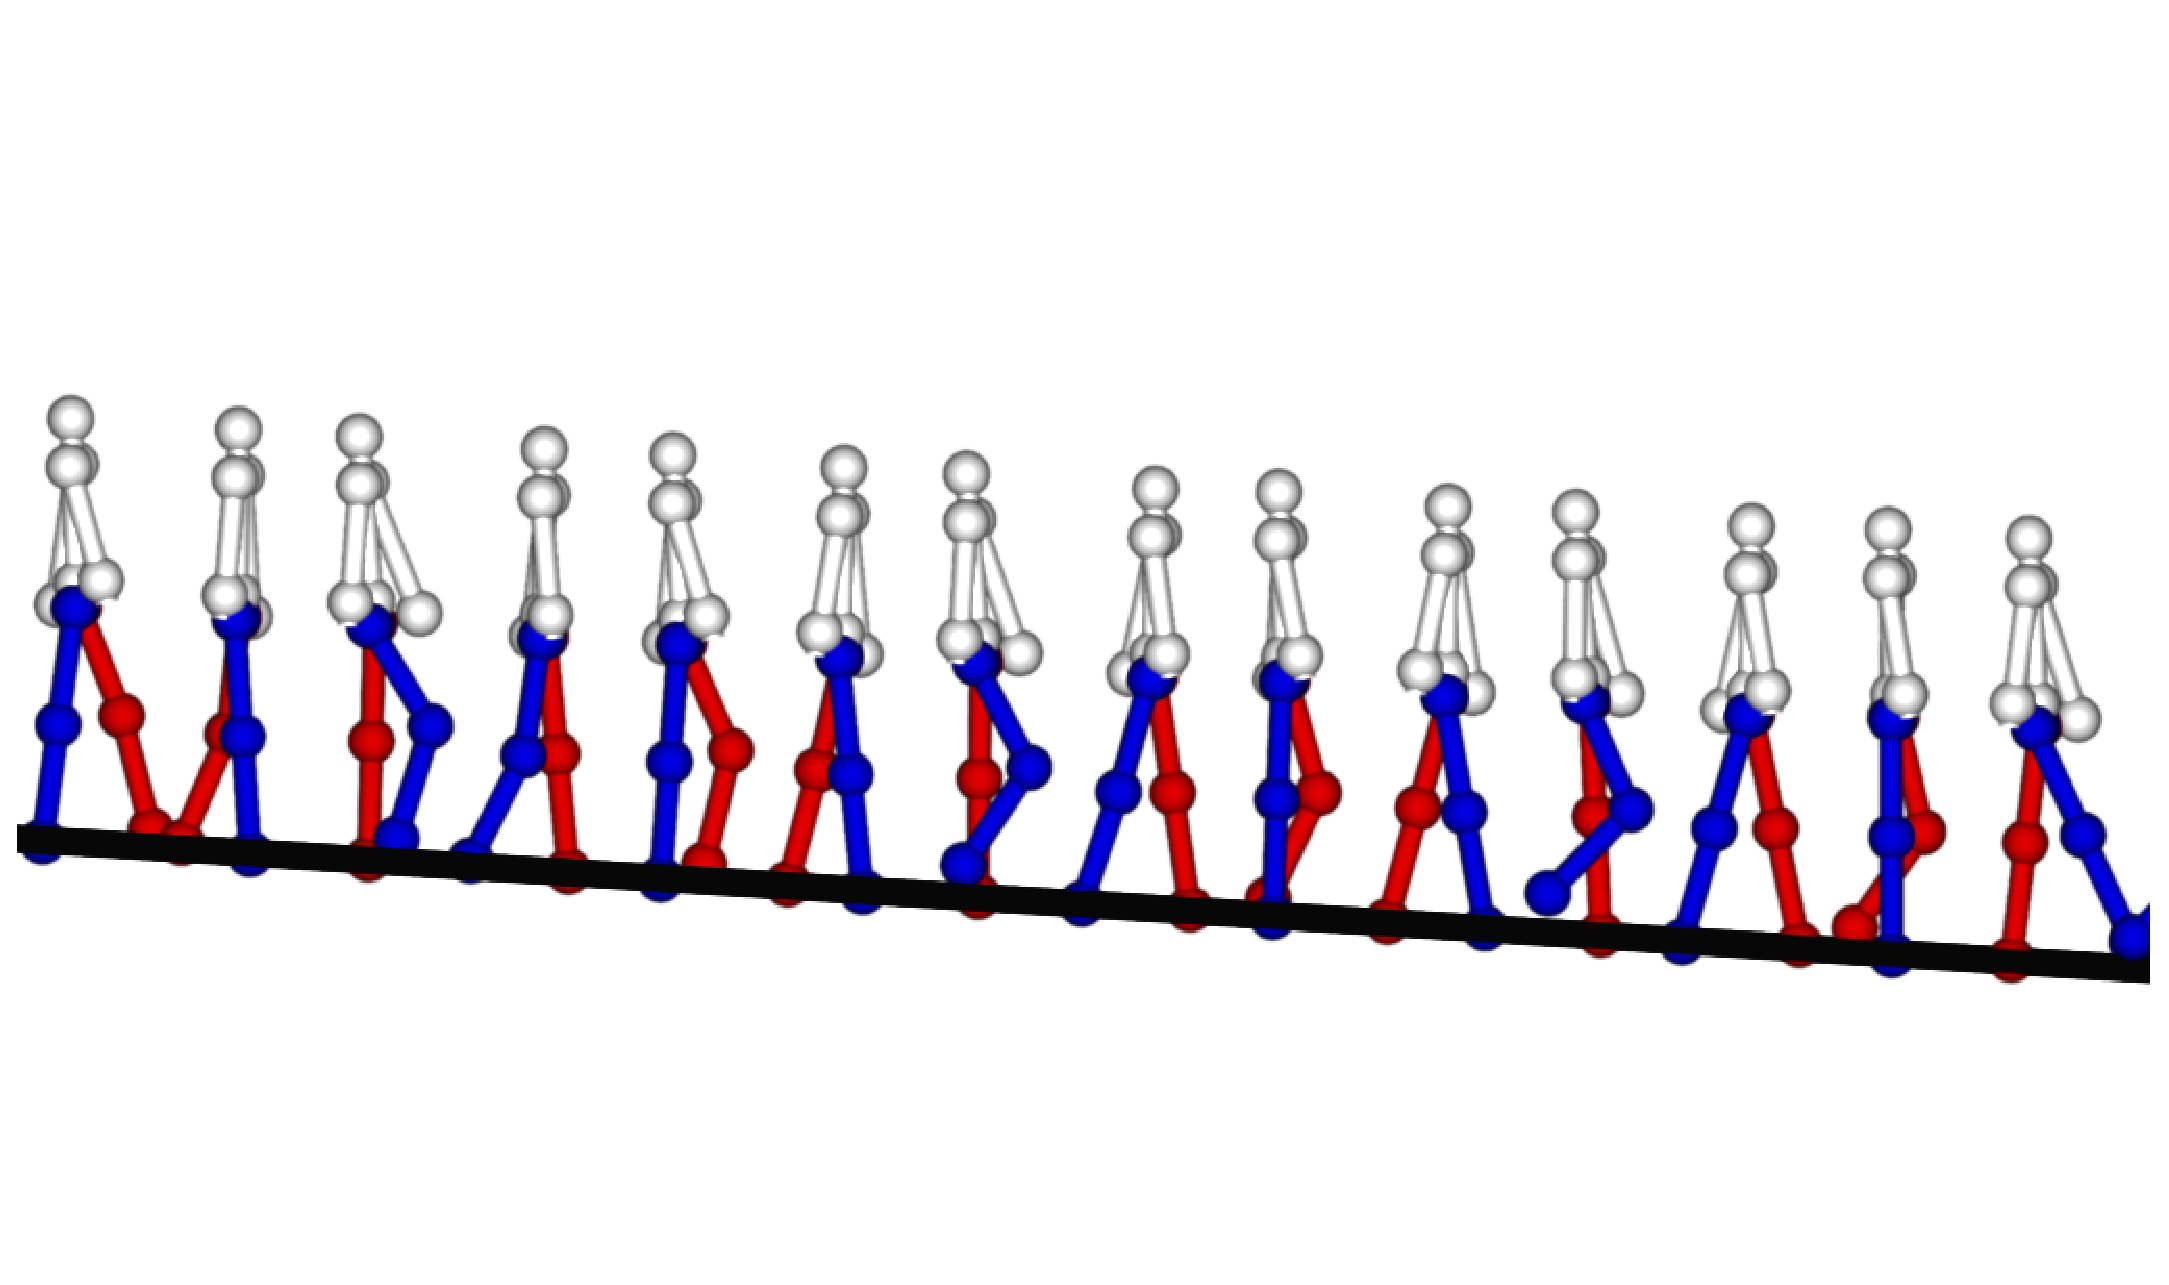
\includegraphics[width=0.7\textwidth]{MLMR130}
    \caption{Gait of $\alpha_b=1.3$}
    \label{fig:lm2}
\end{center}
\end{figure}
As shown in Figure~\ref{fig:differentlr}, when $\alpha_b$ is increased, two legs swing differently and the limit circle is splitted into two.
Bigger $\alpha_b$  will result in a cripple like gait, as shown in Figure~\ref{fig:lm2}



\subsubsection*{Different Slopes}
Usually, changing the slope may not seen as motion re-targeting.
But in \moit, changing slope means changing the parameter of the dynamic equation, which can be analysed in the same manner as as changing body parameters.


Figure ~\ref{fig:diffslopes} shows the limit cycle of walking on different slopes.
For different slopes, entrainment maintains the limit cycle, but the limit cycle changes its shape.
Different stable limit cycles are show in Figure ~\ref{fig:diffslopes}.
Basically, the bigger the slope, the bigger the step size, and the higher the speed.
Slope changing has similar effects to energy scaling.



\begin{figure}[!htbp]
  \begin{center}
      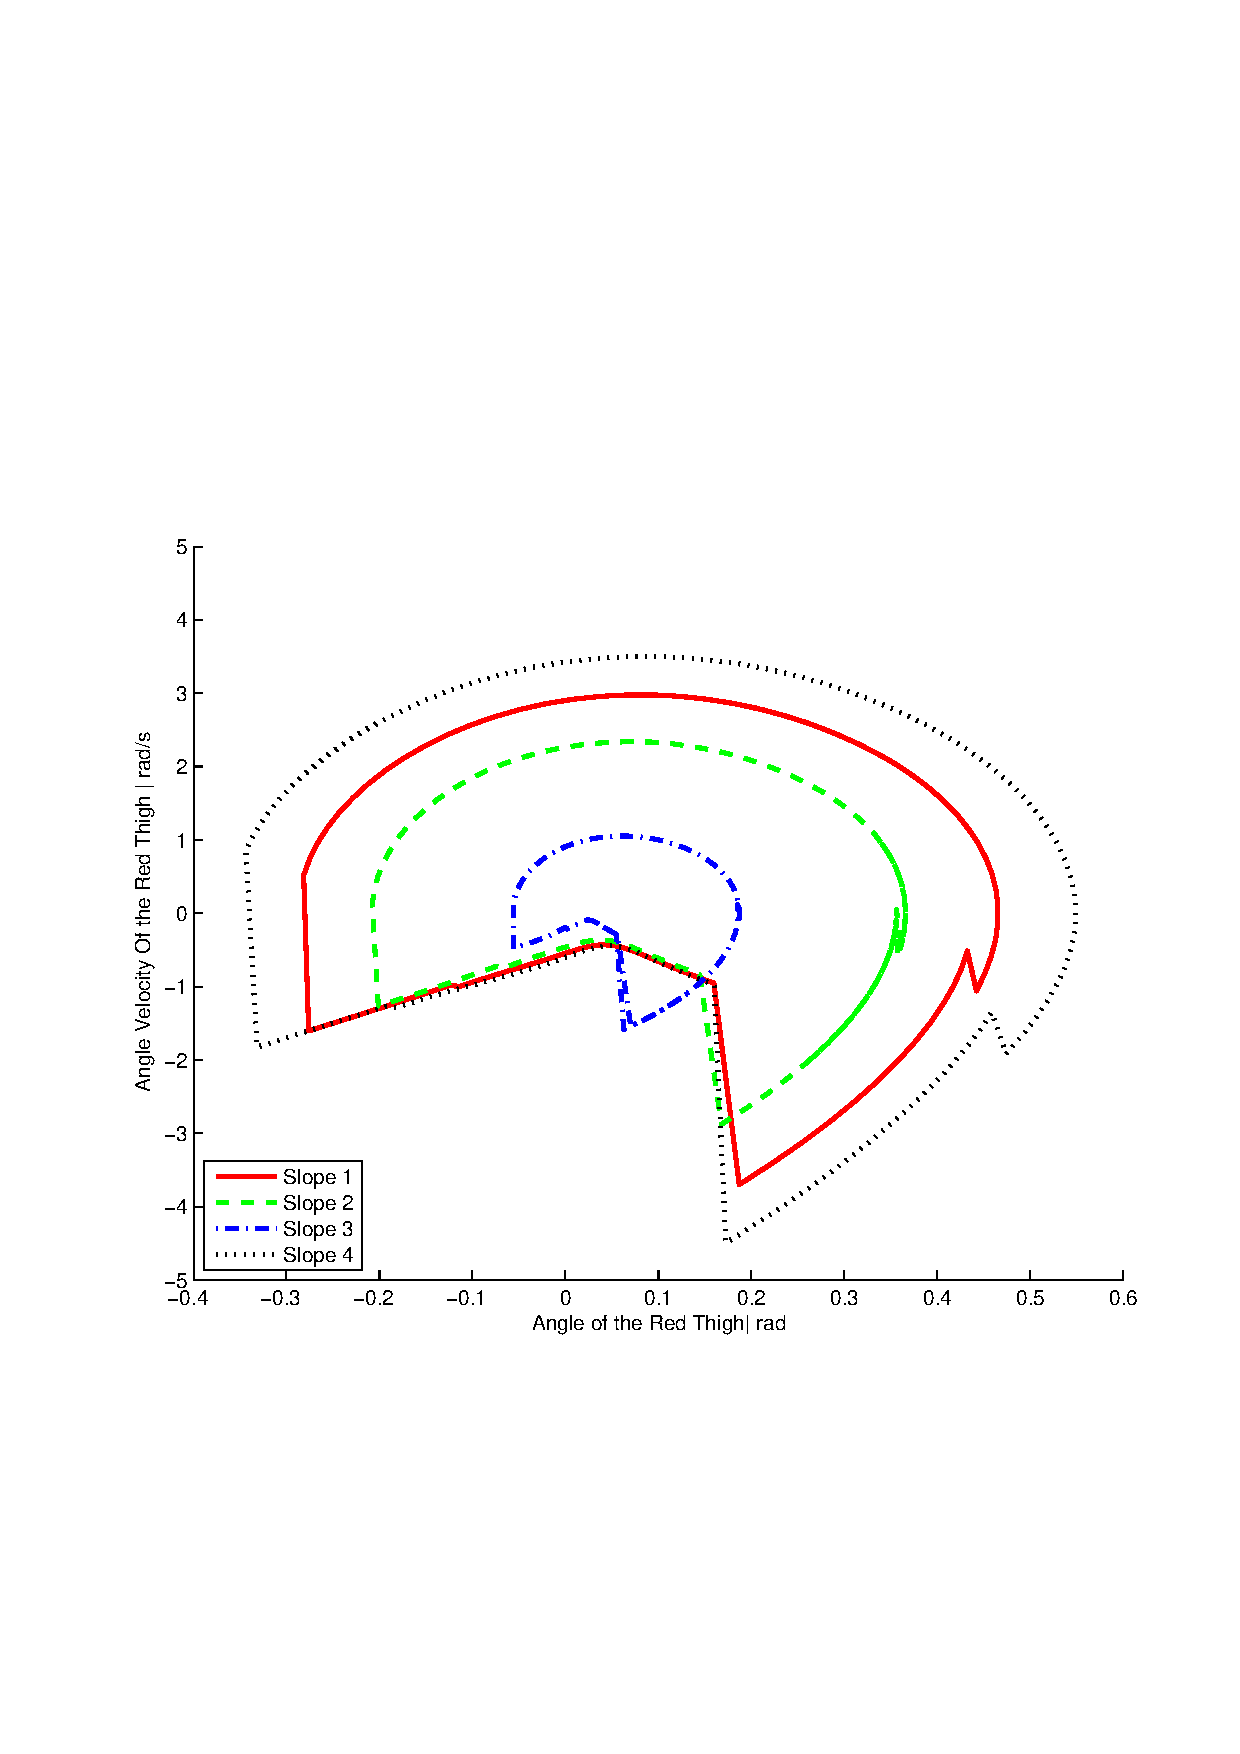
\includegraphics[width=0.7\textwidth]{DifferentSlope}
    \caption{Walking on Different Slopes}
    \label{fig:diffslopes}
\end{center}
\end{figure}

Figure~\ref{fig:ss1},Figure~\ref{fig:ss2} and Figure~\ref{fig:ss3} show different gaits.

\begin{figure}[!htbp]
  \begin{center}
      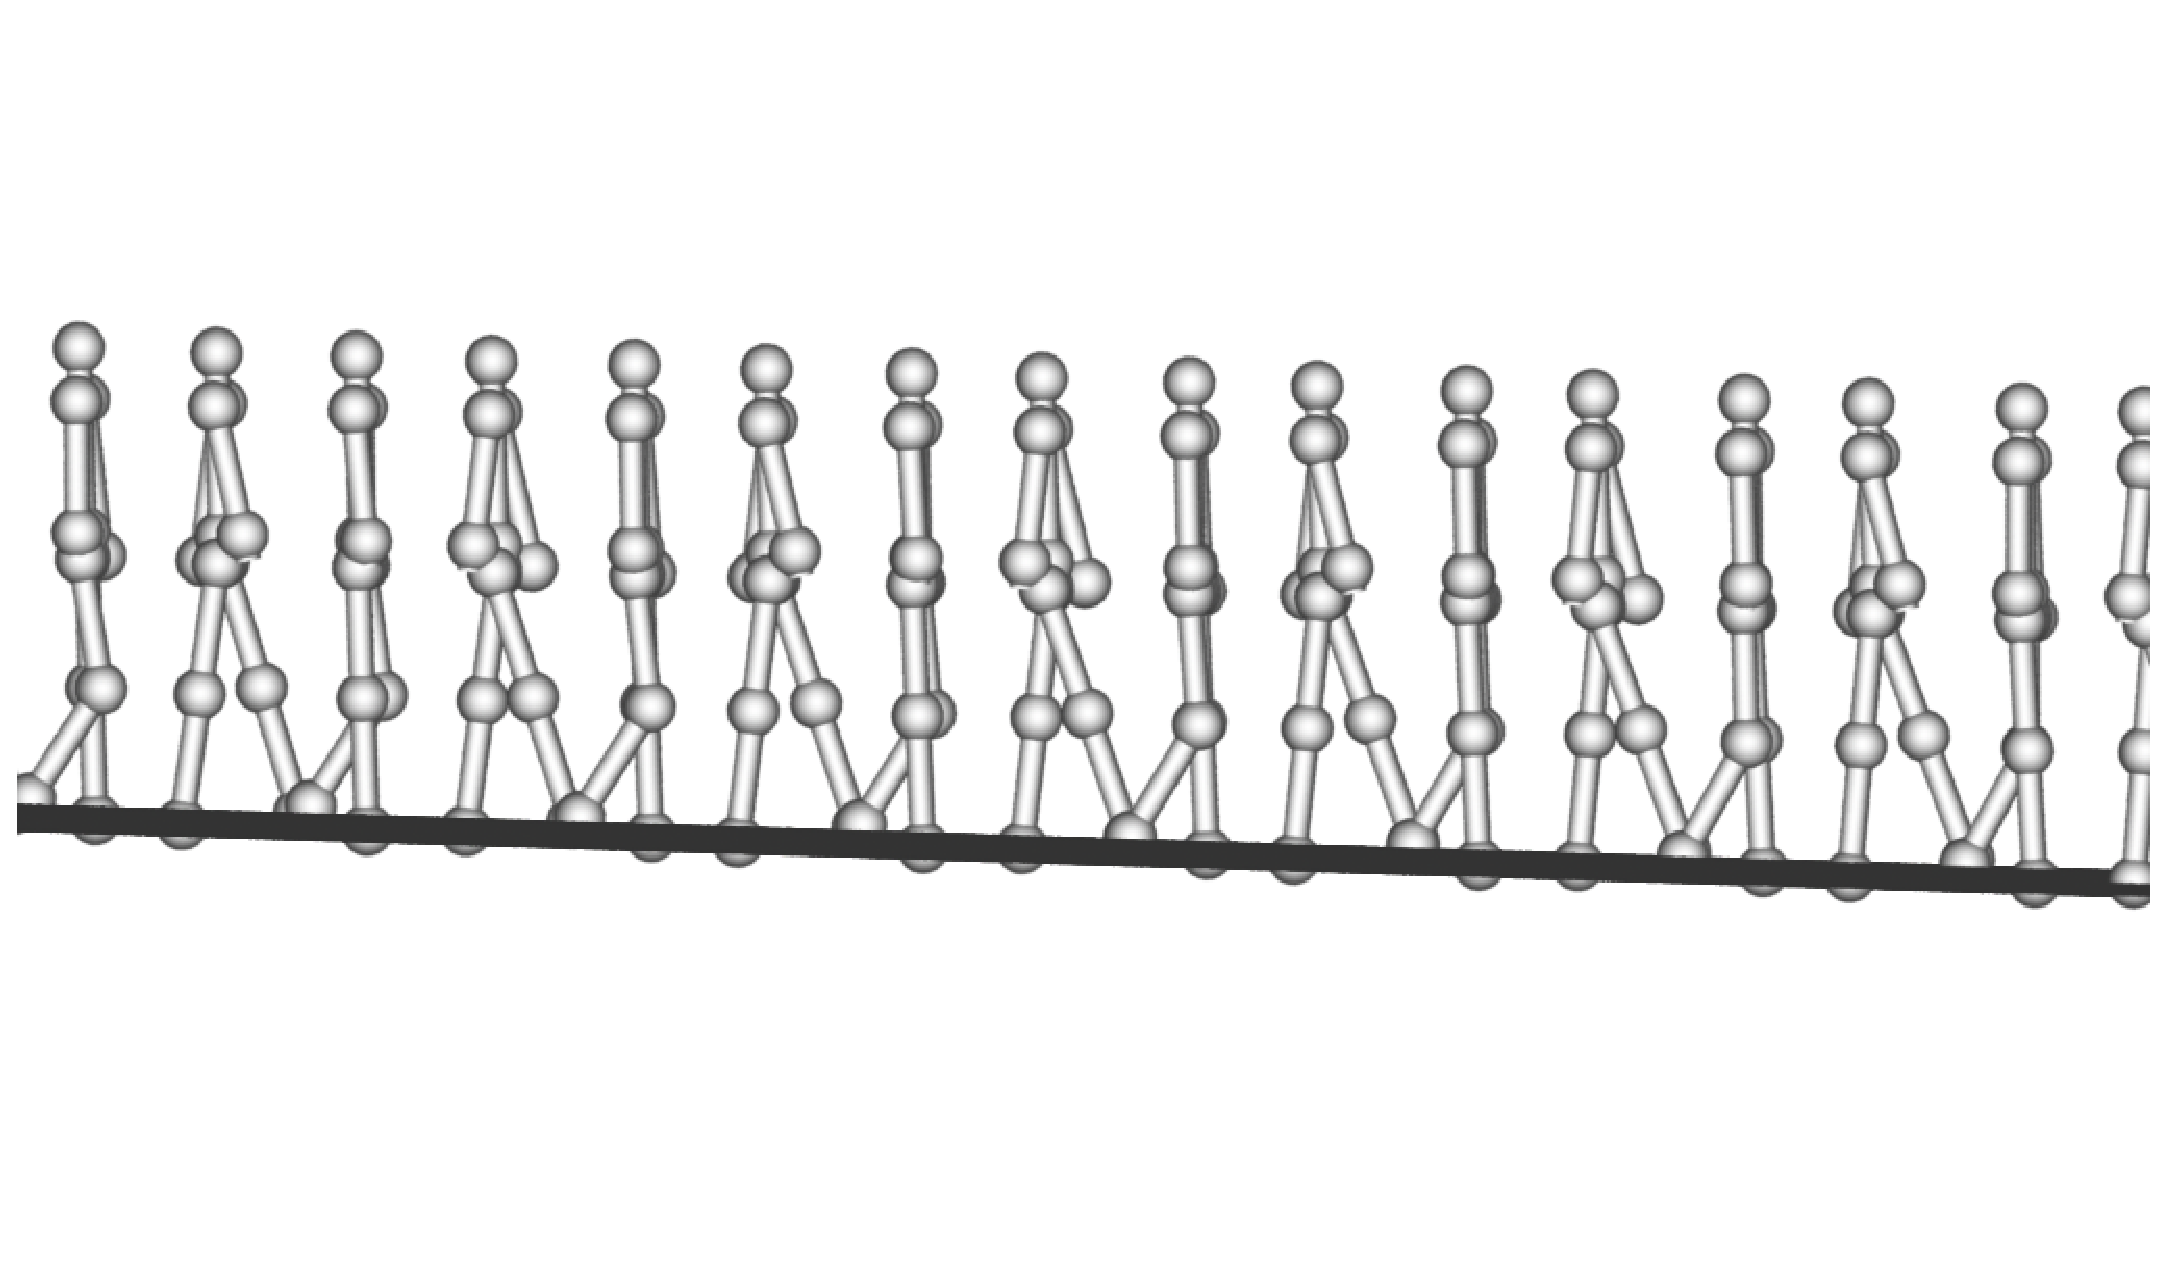
\includegraphics[width=0.7\textwidth]{Slope30}
    \caption{Gait On Slope 1} 
    \label{fig:ss1}
\end{center}
\end{figure}

\begin{figure}[!htbp]
  \begin{center}
      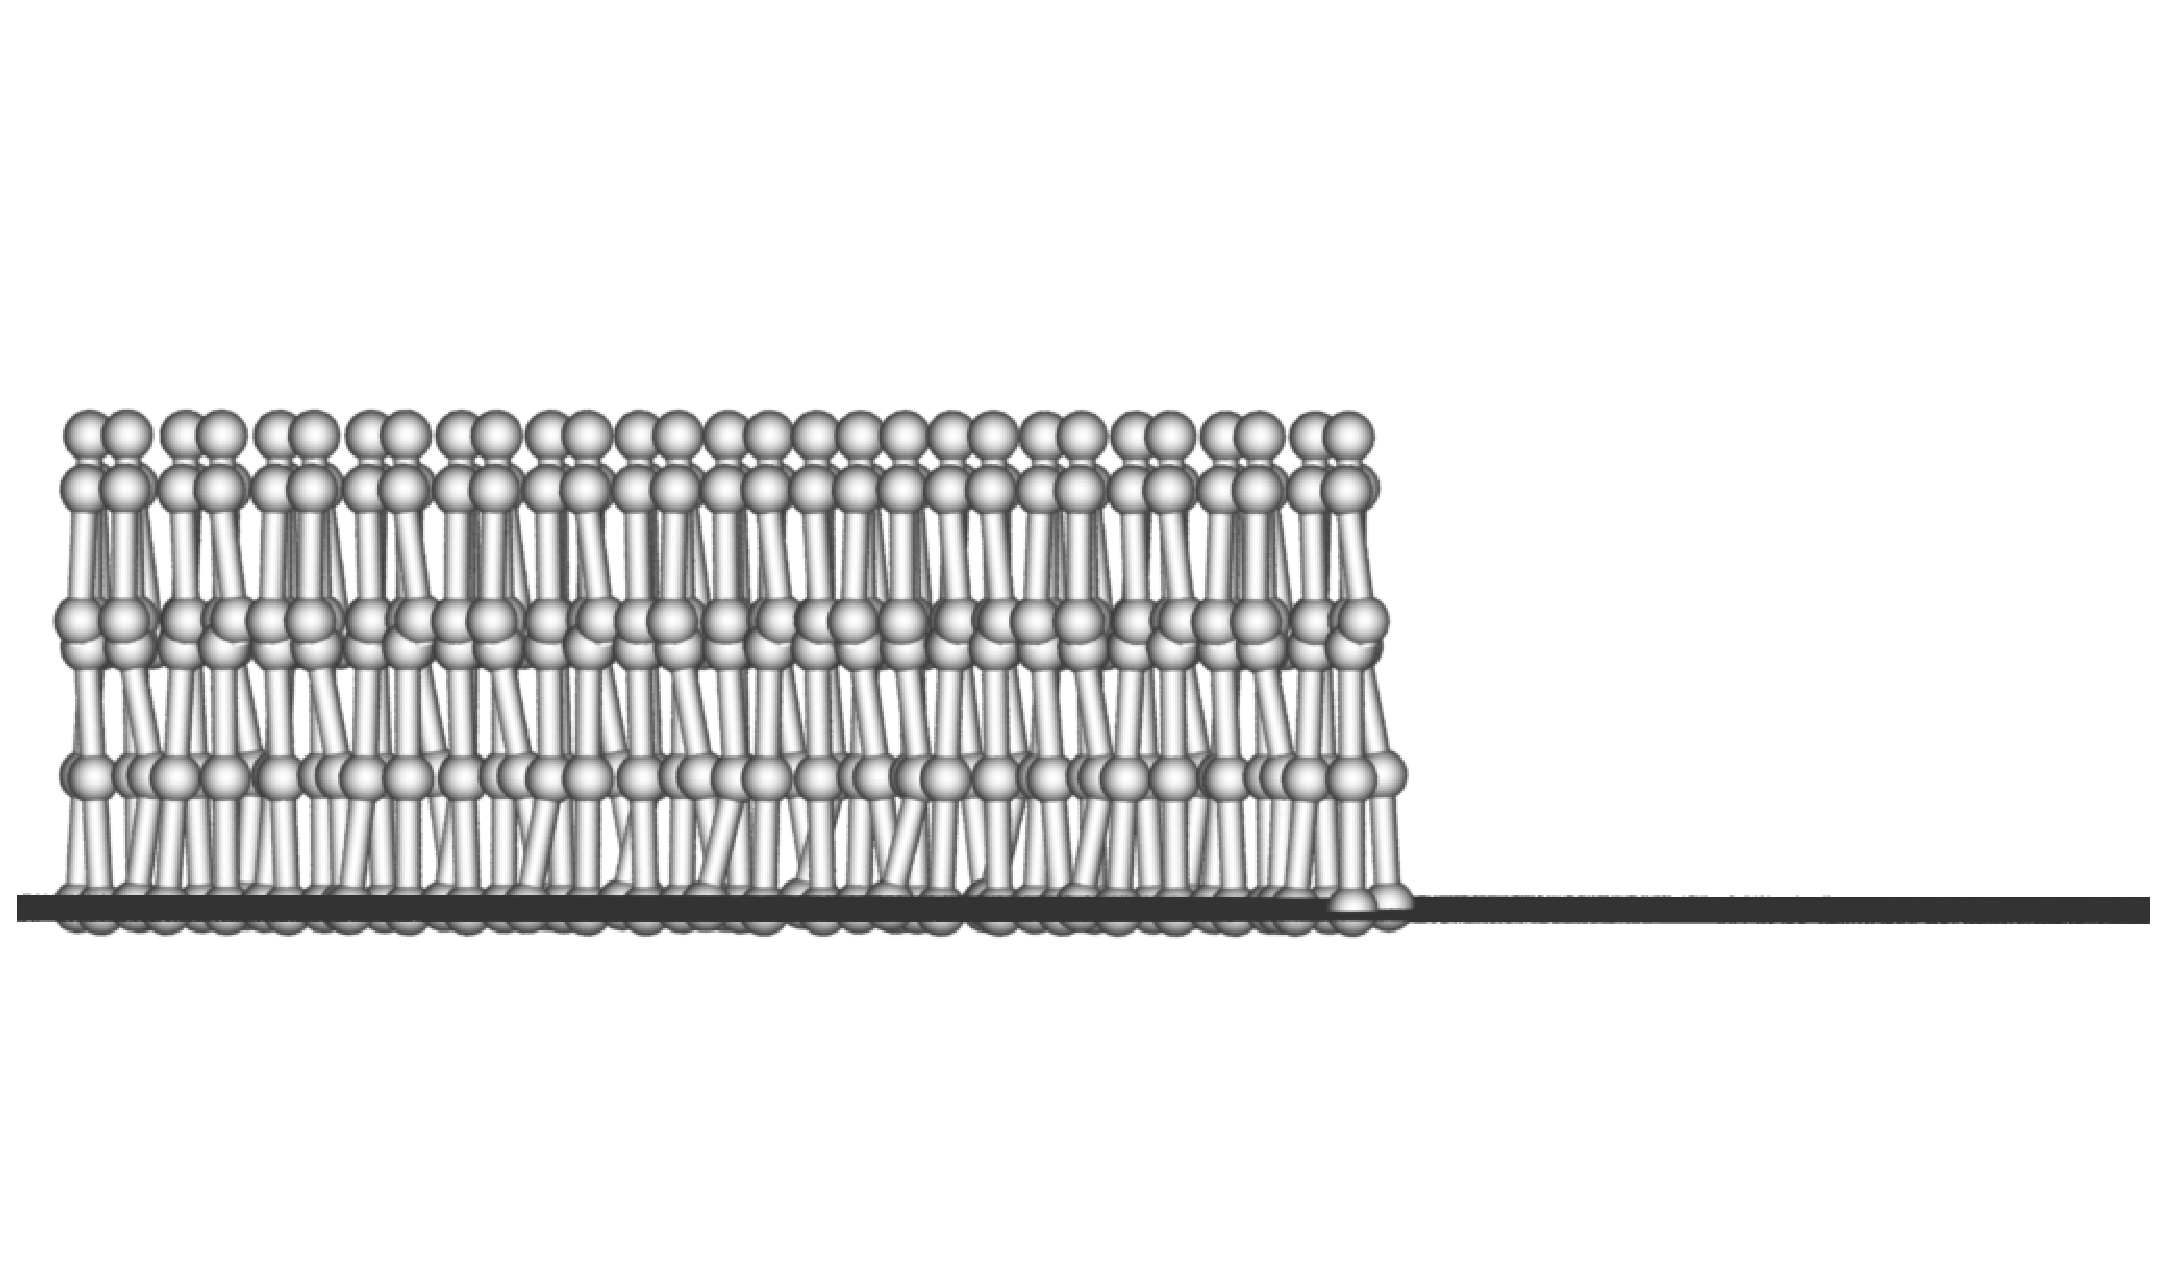
\includegraphics[width=0.7\textwidth]{Slope60}
    \caption{Gait On Slope 2}
    \label{fig:ss2}
\end{center}
\end{figure}

\begin{figure}[!htbp]
  \begin{center}
      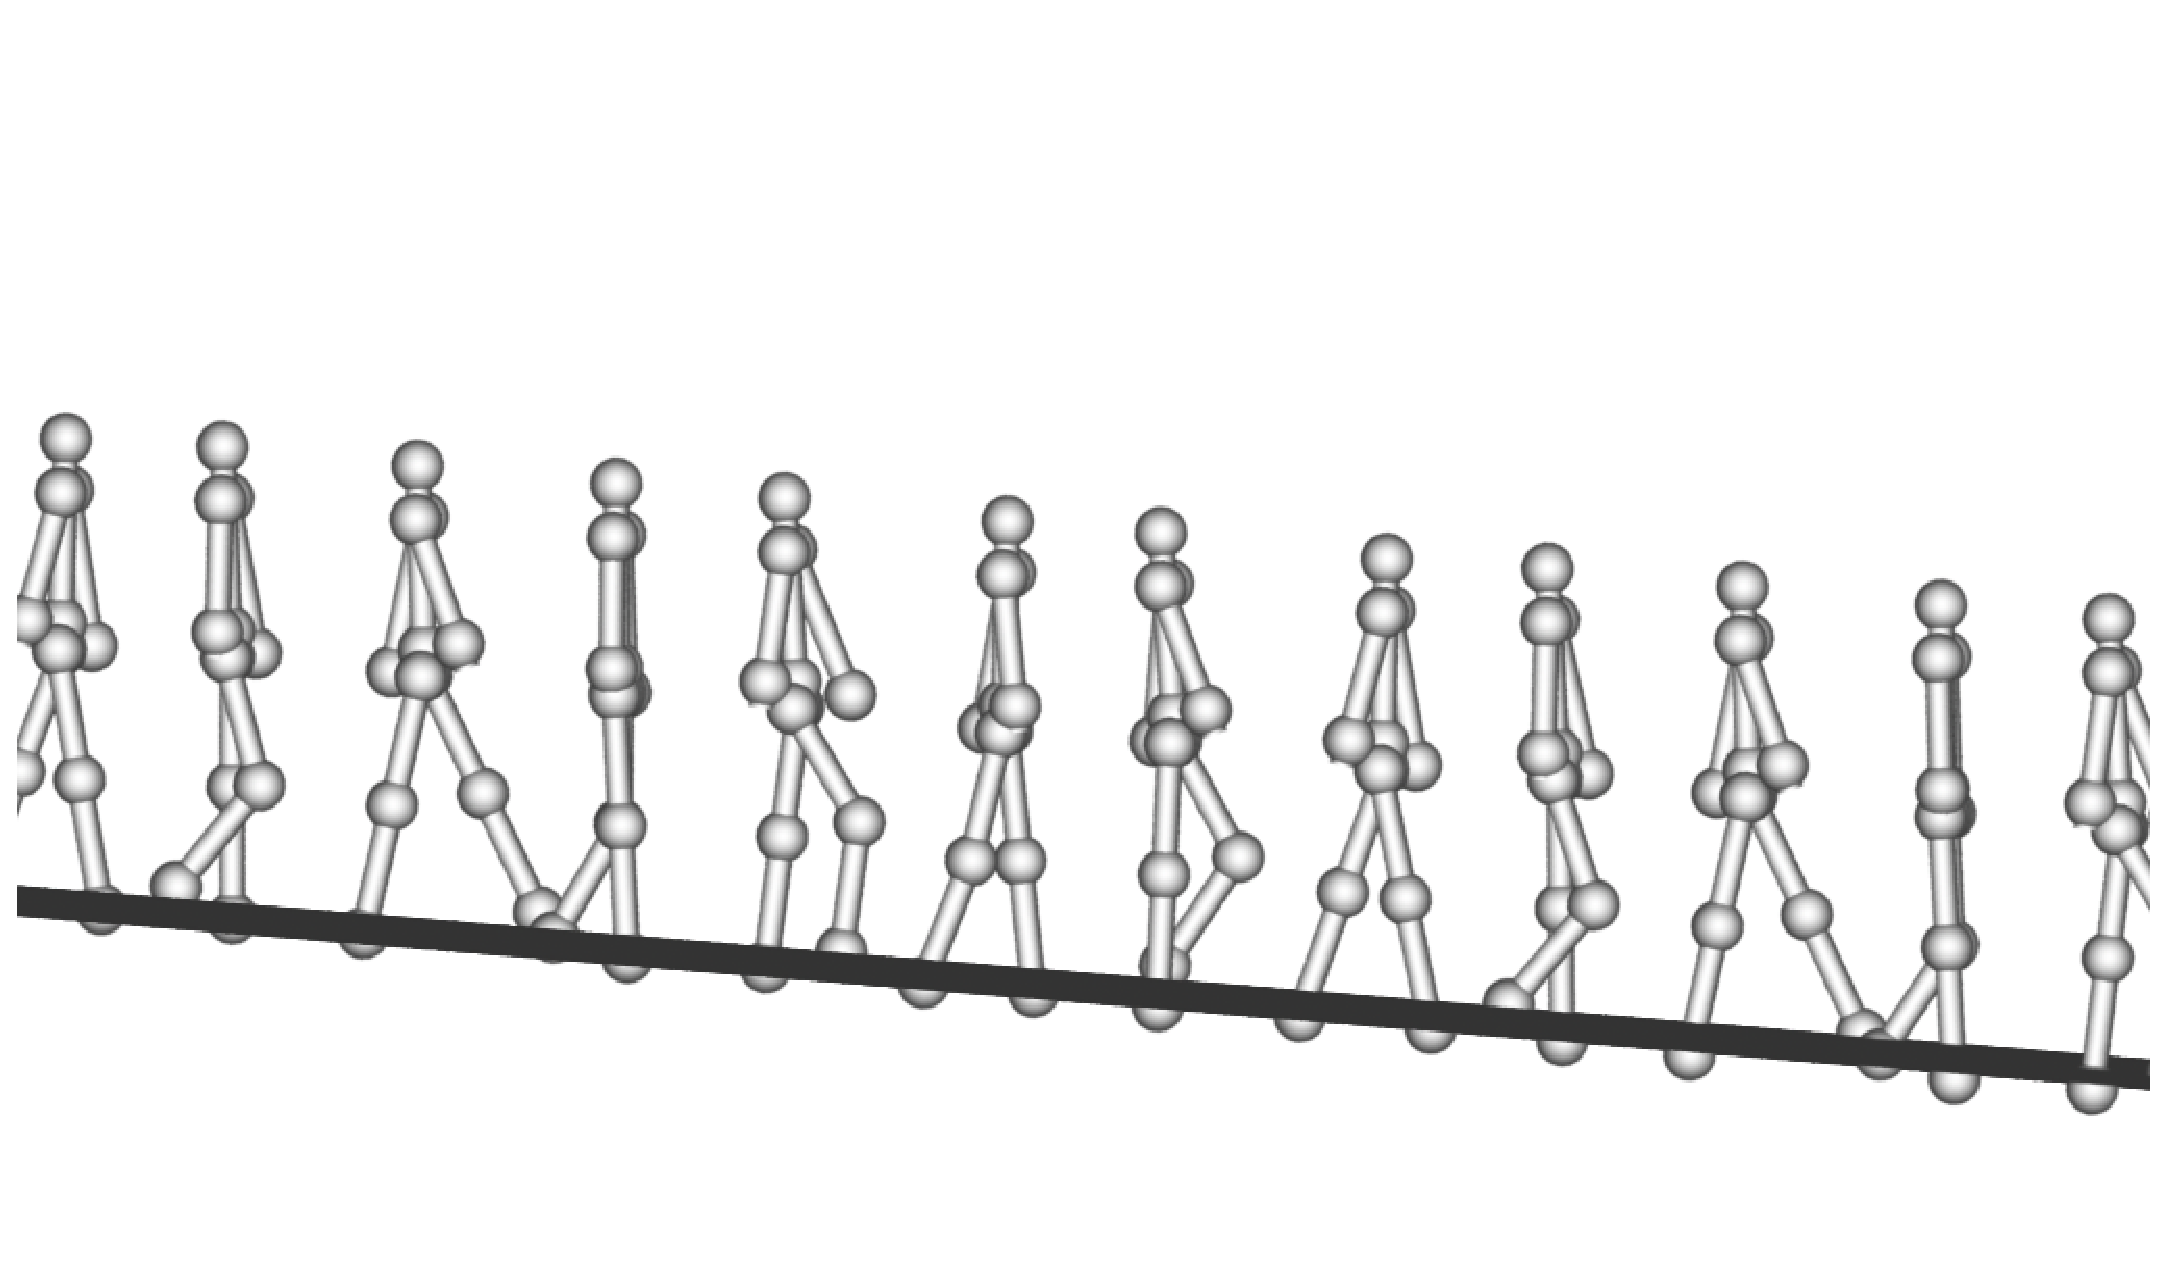
\includegraphics[width=0.7\textwidth]{Slope-20}
    \caption{Gait On Slope 3}
    \label{fig:ss3}
\end{center}
\end{figure}






\section{Local Motor Invariant Control}
Neural Oscillator boosts the stability.
Sometimes stability becomes a limitation in motion.
For the walking example, if the basin of attraction covers the whole space, then the passive walker can't walk upslope.
If the walker is trying to walk upslope, he or she will begin to walk backward down slope after a few steps as shown in Figure~\ref{fig:localcontrolwalking}.
In addition,  it is not convenient to adjust the speed of walking,since the limit cycle is fixed.




\begin{figure}[!htbp]
  \begin{center}
         $\begin{array}{cccc}
\includegraphics[width=1in]{UpFall/0001.eps}&
\includegraphics[width=1in]{UpFall/0051.eps}&
\includegraphics[width=1in]{UpFall/0101.eps}&
\includegraphics[width=1in]{UpFall/0151.eps}
\\
\includegraphics[width=1in]{UpFall/0201.eps}&
\includegraphics[width=1in]{UpFall/0251.eps}&
\includegraphics[width=1in]{UpFall/0301.eps}&
\includegraphics[width=1in]{UpFall/0351.eps}
\end{array}$
    \caption{Failure of walking upslope}
    \label{fig:localcontrolwalking}
\end{center}
\end{figure}

Local Motor Invariant provides a mechanism to adapt motion according to the environment and application-specific purpose. 
For the bipedal walking, group actions provides a mechanism to adjust the walking slope and walking speed in precision.




\subsection{Group Actions}

Equation~\ref{eq:localcontrolwalking} describes walking with local control.
\begin{equation}
\label{eq:localcontrolwalking}
M(\mathbf{q}) \ddot{\mathbf{q}} + C(\mathbf{q,\qd})\dot{\mathbf{q}} + N(\mathbf{q}) = \ulocal
\end{equation}




Lie group actions are developed for two types of symmetry.
\begin{itemize}

\HiItem{Offset Action}.
Offset Action moves the phase plot horizontally.
This will make the passive walking on terrains of different slopes.
For the bipedal walking, the offset action is:
\[
\ulocal=N(q)-N(q+\ep)
\]
\HiItem{Speed Action}
Speed Action maintains the gait, but modifies the walking speed.
The local control is:
\[  
\ulocal=(1-\ep^2)N
\]
\end{itemize}

The original system does not have energy scaling symmetry.
Energy Scaling is approximated by a combined method discussed later.

Figure~\ref{fig:walkliegroupphase} demonstrates different limit cycles after applying lie group actions.
The red one is the original limit cycle.
Green ones are applied offset actions and blue ones are applied speed actions.


\begin{figure}[!htbp]
  \begin{center}
     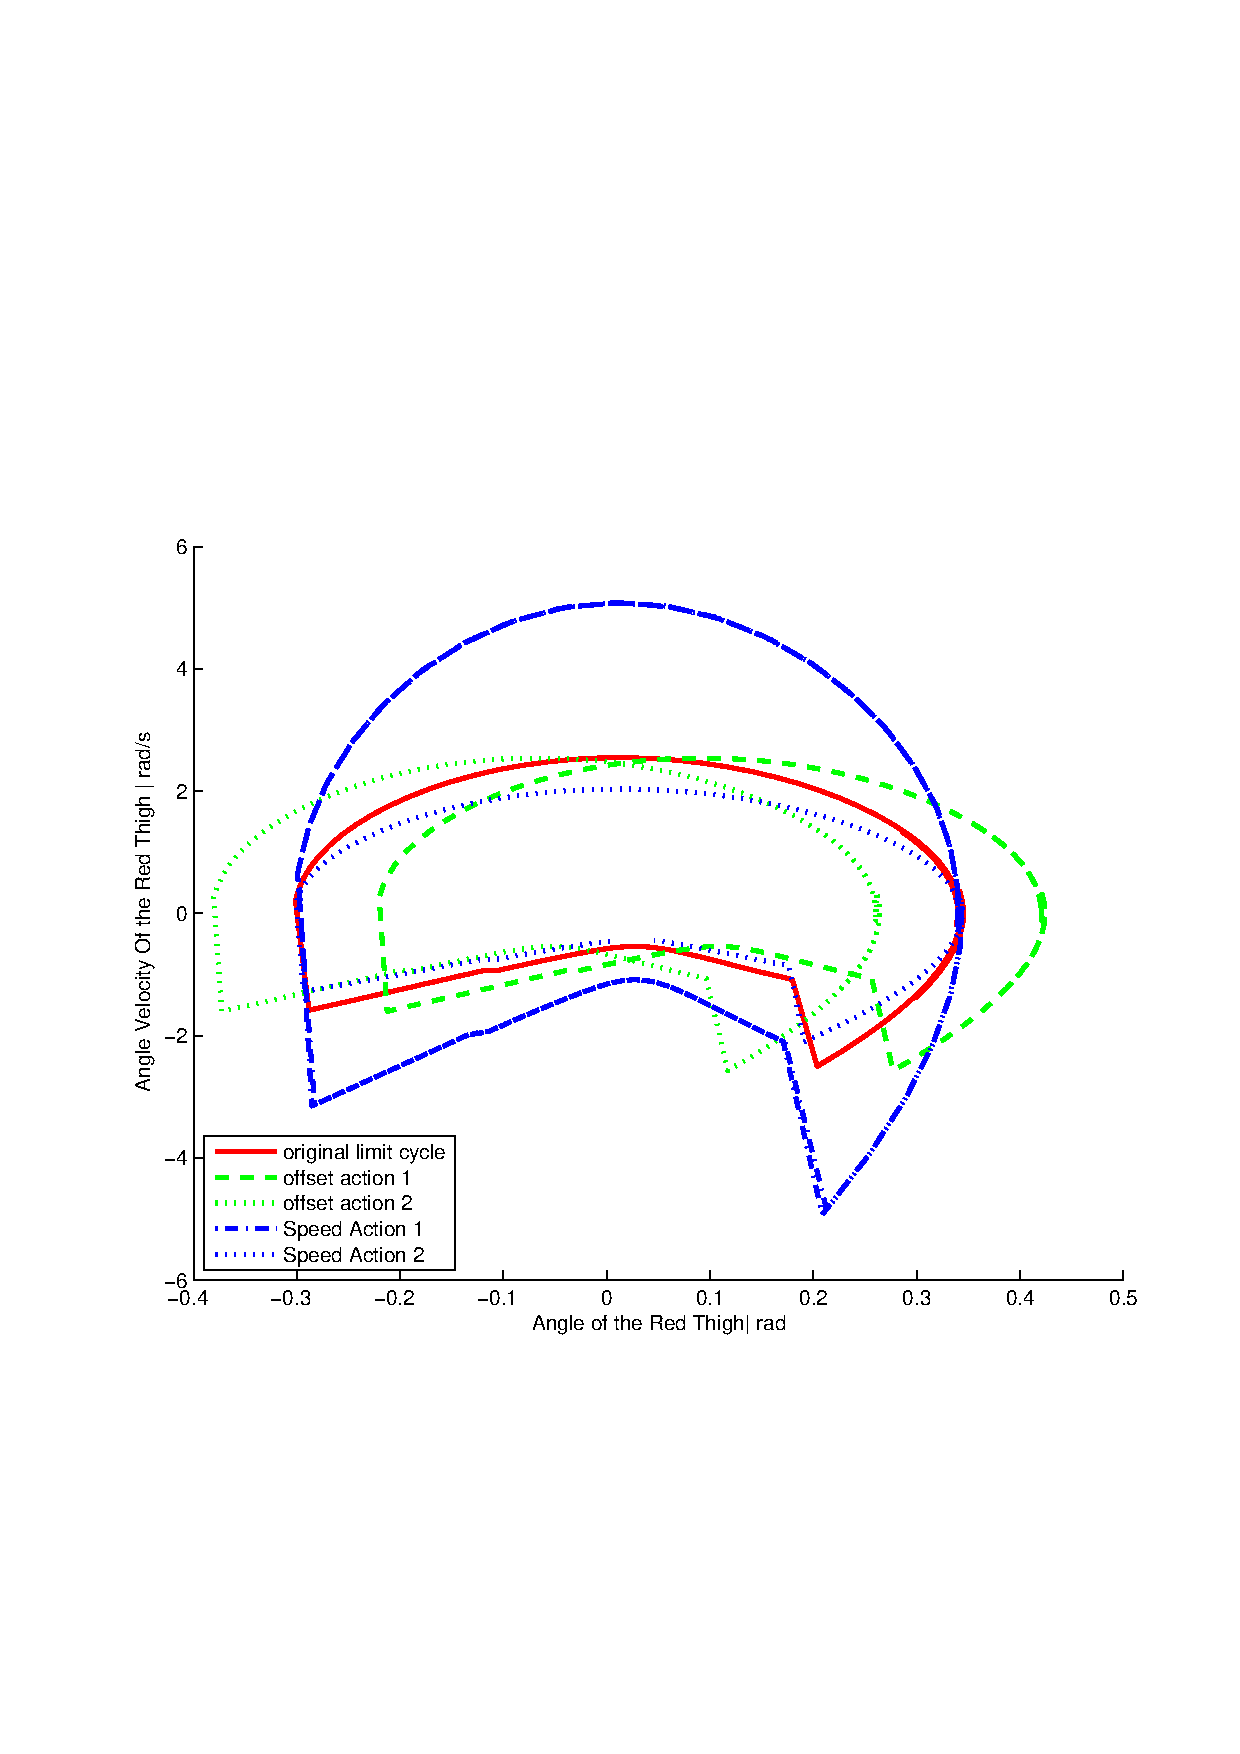
\includegraphics[width=0.7\textwidth]{LieGroupAction}
    \caption{Lie Group Actions on the Phase Plot}
    \label{fig:walkliegroupphase}
\end{center}
\end{figure}


By applying the offset action,   the passive walker can walk upslope, as shown in Figure~\ref{fig:liegroupupslope}
\begin{figure}[!htbp]
  \begin{center}
      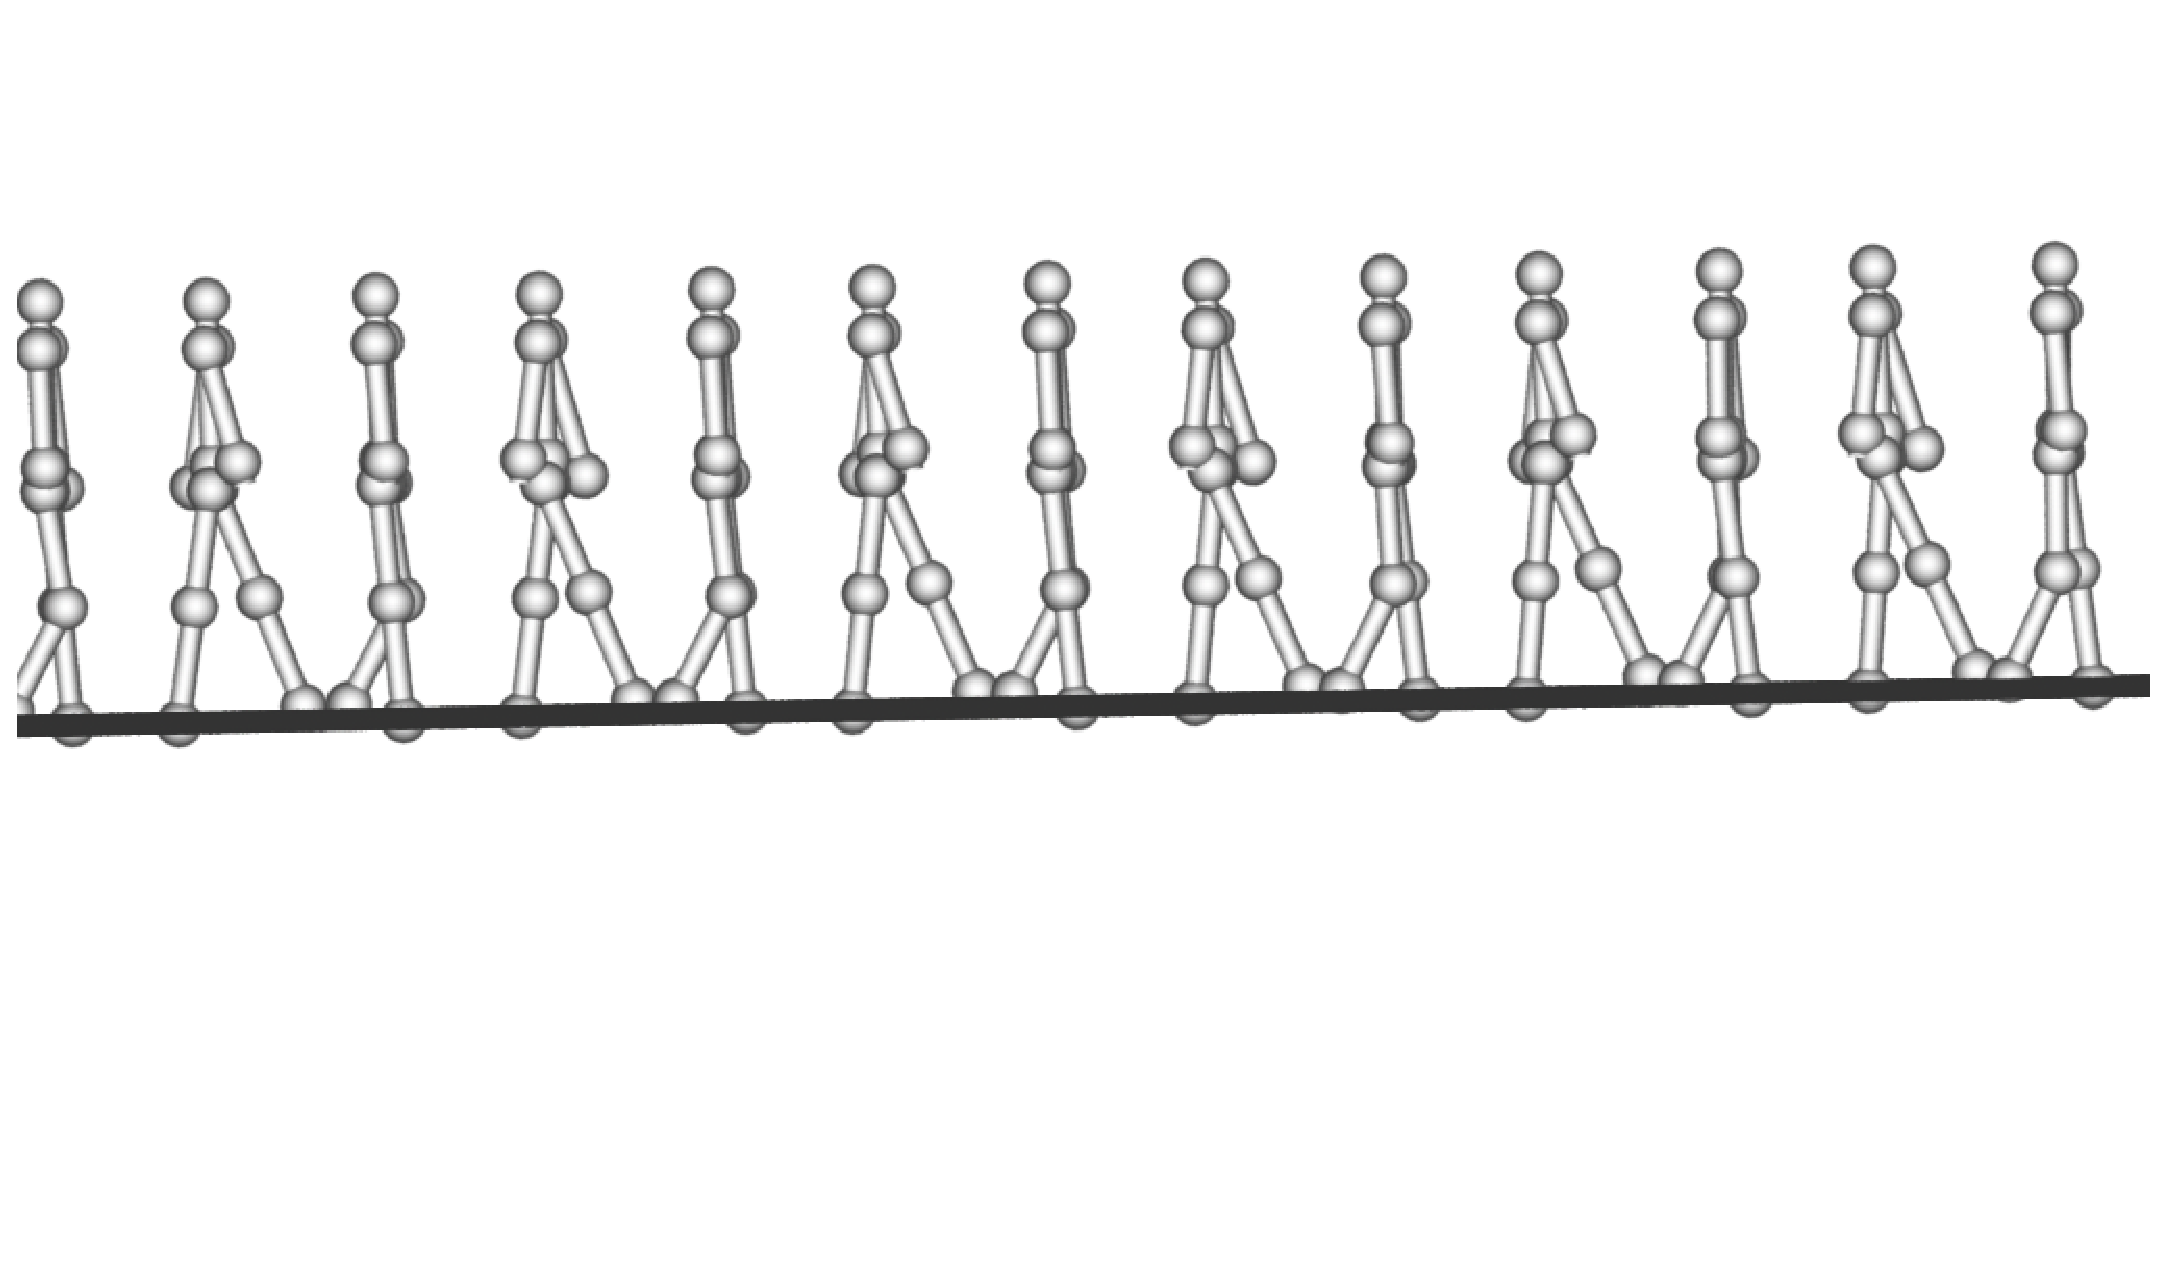
\includegraphics[width=0.7\textwidth]{LieUpslope}
    \caption{Up slope Gait Generate by Lie Group offset Action}
    \label{fig:liegroupupslope}
\end{center}
\end{figure}

\section{Application of Combined Method}
Global Motor Invariant Control boosts the walking stability.
However,  the resulting motion does not meet application's needs sometimes.
Local Motor Invariant Control can adapt the walking to application purpose, but it can't boost the stability.
Combining the two controllers make it possible to take the strengths of the two methods.

The combined method is described by Equation~\ref{eq:combinedcontrolwalking}
\begin{equation}
\label{eq:combinedcontrolwalking}
M(\mathbf{q}) \ddot{\mathbf{q}} + C(\mathbf{q,\qd})\dot{\mathbf{q}} + N(\mathbf{q}) = D\uout+\ulocal
\end{equation}

In applications, animator can generate different gaits through  adjusting  parameters of the neural oscillator and the body first, and then transform the different gaits by lie group actions.
For animators, this method is efficient, natural looking and easy to use.

Such combinations will achieve unlimited variations of gaits.
We will demonstrate below how gait variations can be achieved in this manner.

\subsection{Step Size Adjust}
The first example shows how a character can adjust his step size realistically.
When the character walks down different slopes, a steeper slope will result in a bigger step size as shown in Figure~\ref{fig:diffslopes}. 
If an offset Lie group actions is applied, we can transform the gaits of different slopes on the plane.
In this way we can achieve different step gaits on the plane.

Figure~\ref{fig:differentstepsizeonplaine} shows limit cycles of different step size on the plane.
\begin{figure}[!htbp]
  \begin{center}
      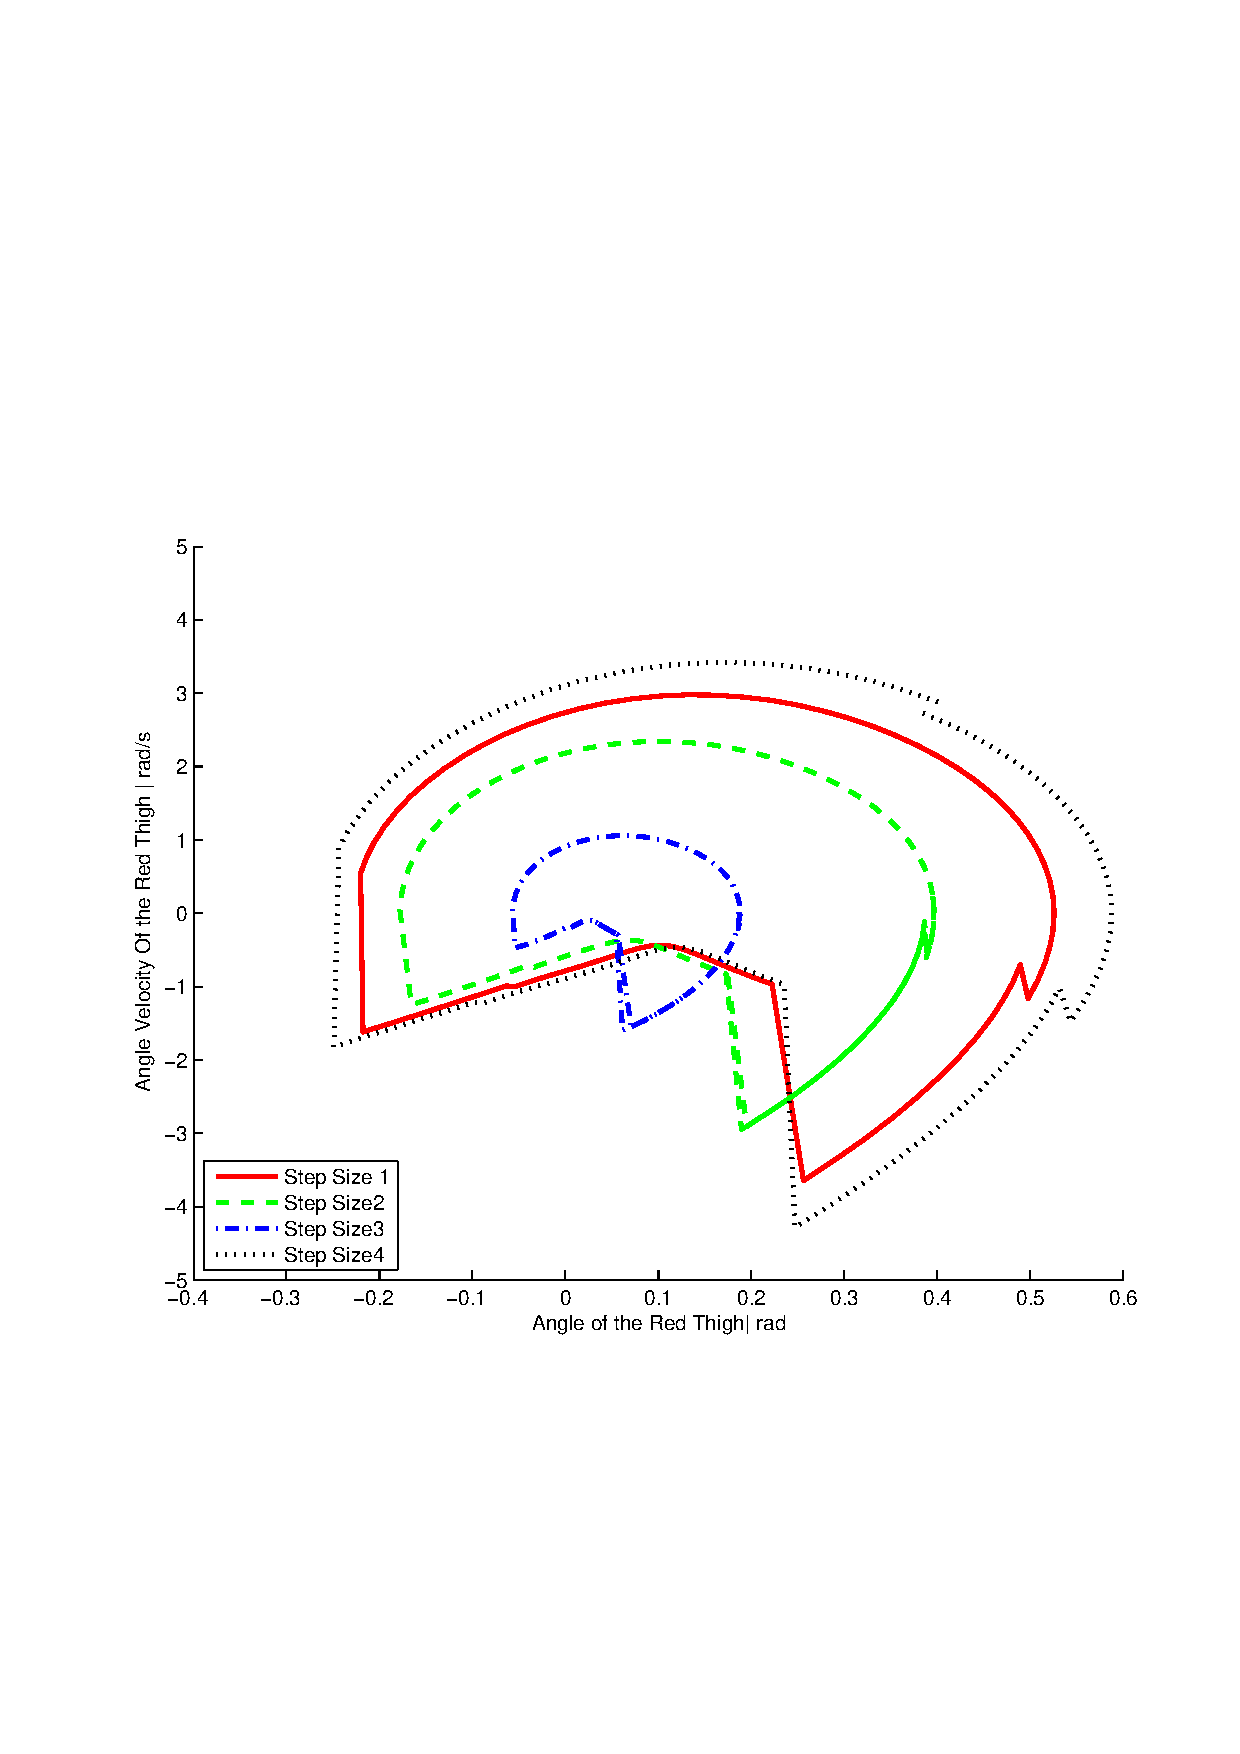
\includegraphics[width=0.7\textwidth]{DifferentStepSizeWalking}
    \caption{Limit Cycles of Different Step Size Gaits}
    \label{fig:differentstepsizeonplaine}
\end{center}
\end{figure}


And the different gaits are shown in Figure~\ref{fig:ssp1},Figure~\ref{fig:ssp2} and Figure~\ref{fig:ssp3}.
\begin{figure}[!htbp]
  \begin{center}
      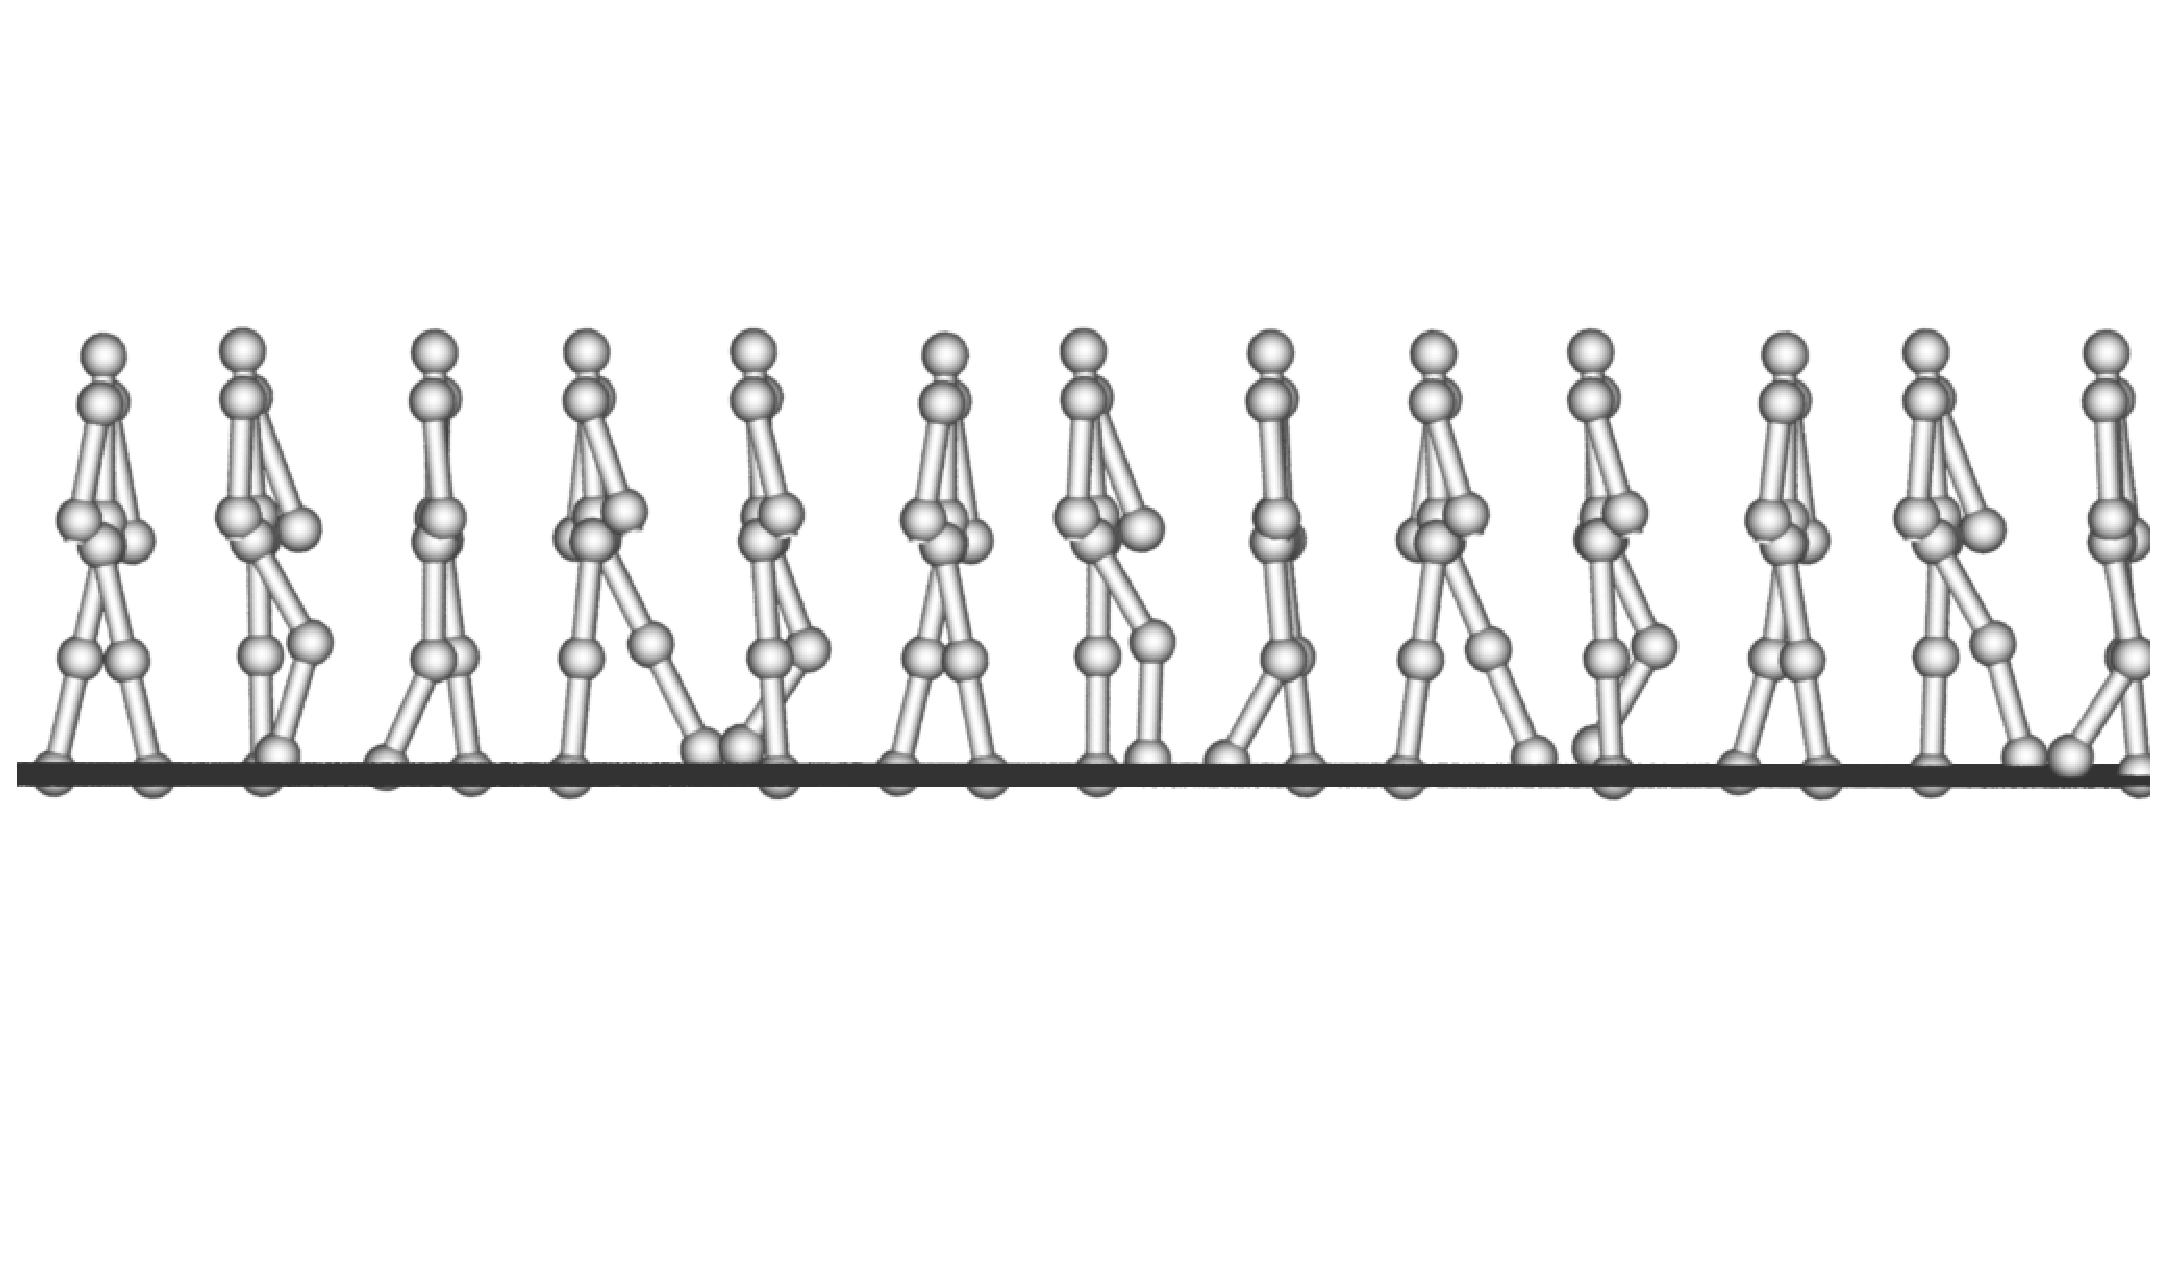
\includegraphics[width=0.7\textwidth]{stepsize1}
    \caption{gait with step size 1}
    \label{fig:ssp1}
\end{center}
\end{figure}

\begin{figure}[!htbp]
  \begin{center}
      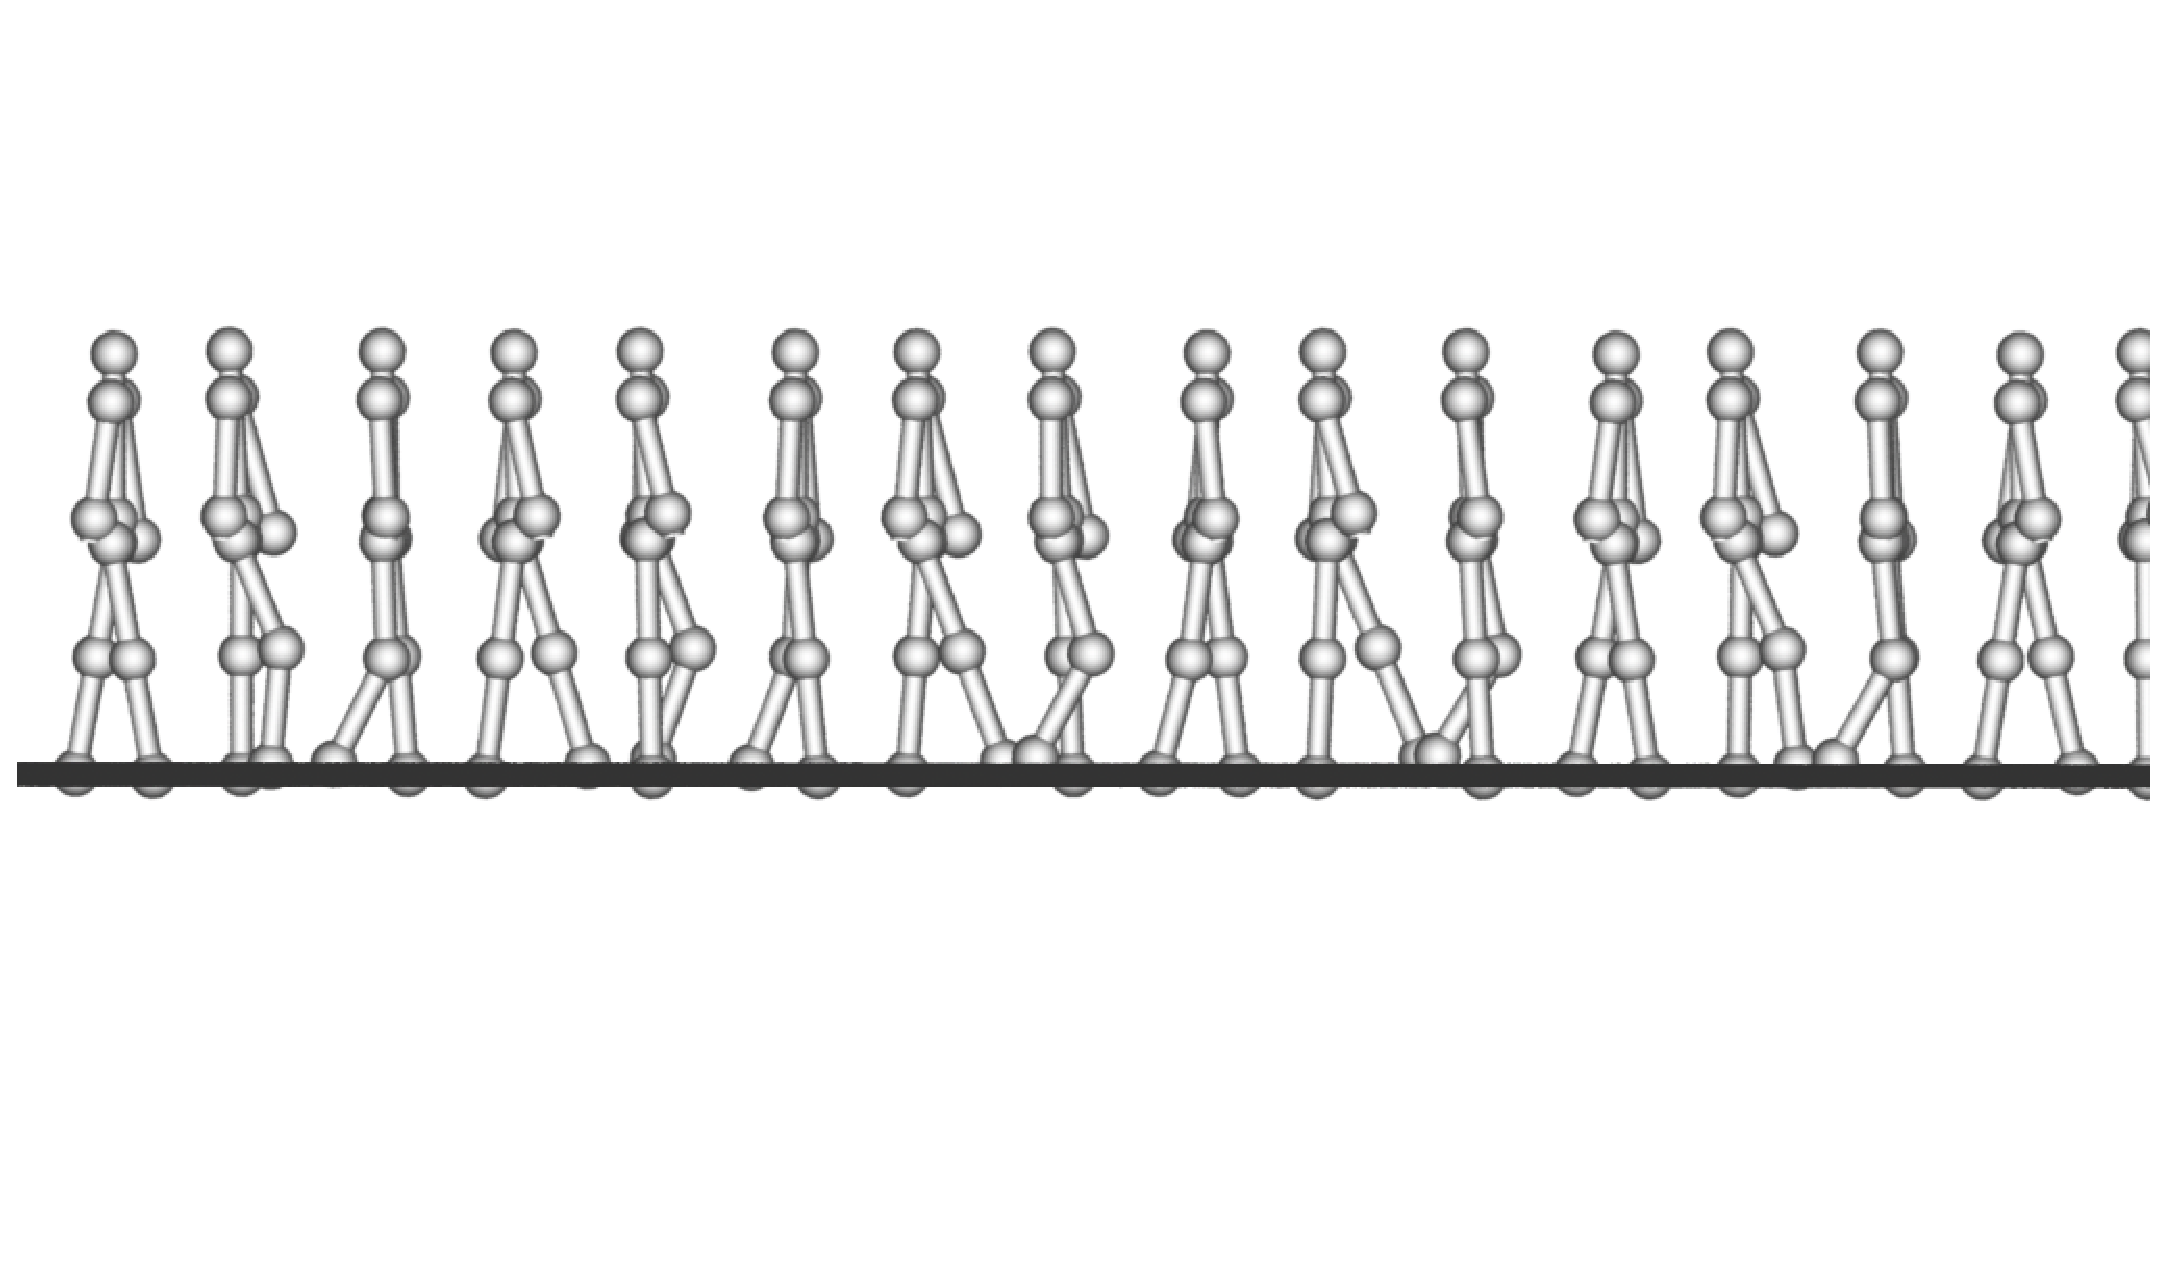
\includegraphics[width=0.7\textwidth]{stepsize2}
    \caption{gait with step size 2}
    \label{fig:ssp2}
\end{center}
\end{figure}

\begin{figure}[!htbp]
  \begin{center}
      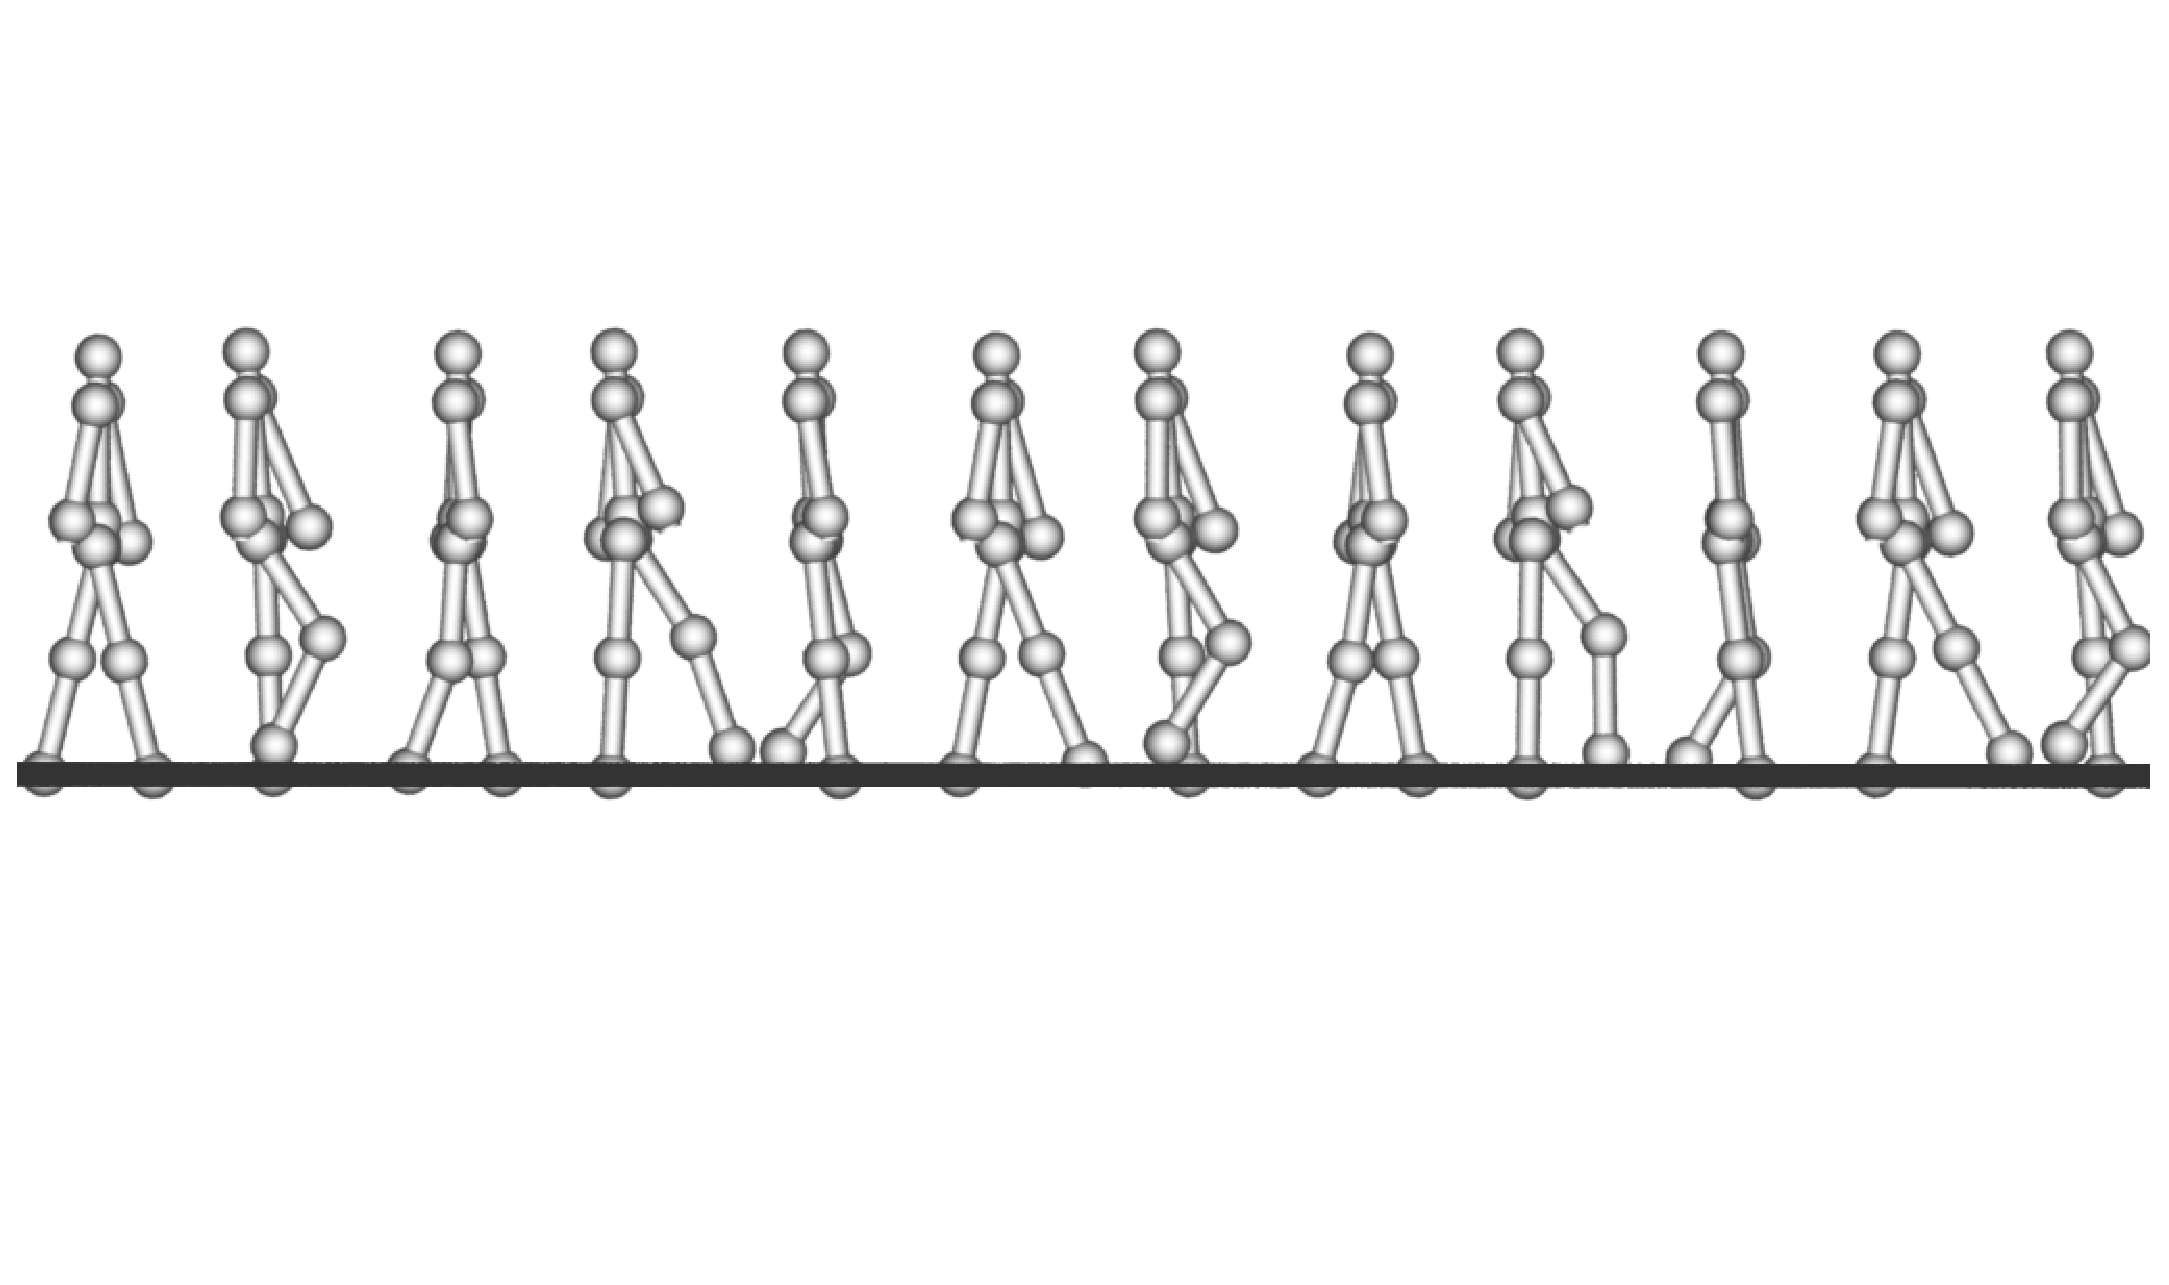
\includegraphics[width=0.7\textwidth]{stepsize4}
    \caption{gait with step size 4}
    \label{fig:ssp3}
\end{center}
\end{figure}







\subsection{Varying Slopes}
Neural Oscillator can maintain walking on varying slopes, but can't make a character walk up slope.
Lie Group action allow the character to walk up a slope with a constant angle.
However varying the slope will result in walking failure.
By combining the two methods, the passive walker can walk on terrains of varying slopes.


The control strategy is straight forward.
Lie group action is maintained on each plane.
During a slope transition, controller looks ahead and sets the lie group action for  walking on the slope for the next step.
At transition, the state will move far away from the stable limit cycle, and need a few steps to converge to the limit circle.
This result in gait adjustment.
Sometimes, character will take a few small steps and increase it to normal steps later.


Figure~\ref{fig:vp1} and Figure~\ref{fig:vp2} show the gaits on smooth slopes.
The phase plot of gaits in Figure~\ref{fig:vp1} is shown in Figure~\ref{fig:vp2phas}.

\begin{figure}[!htbp]
  \begin{center}
      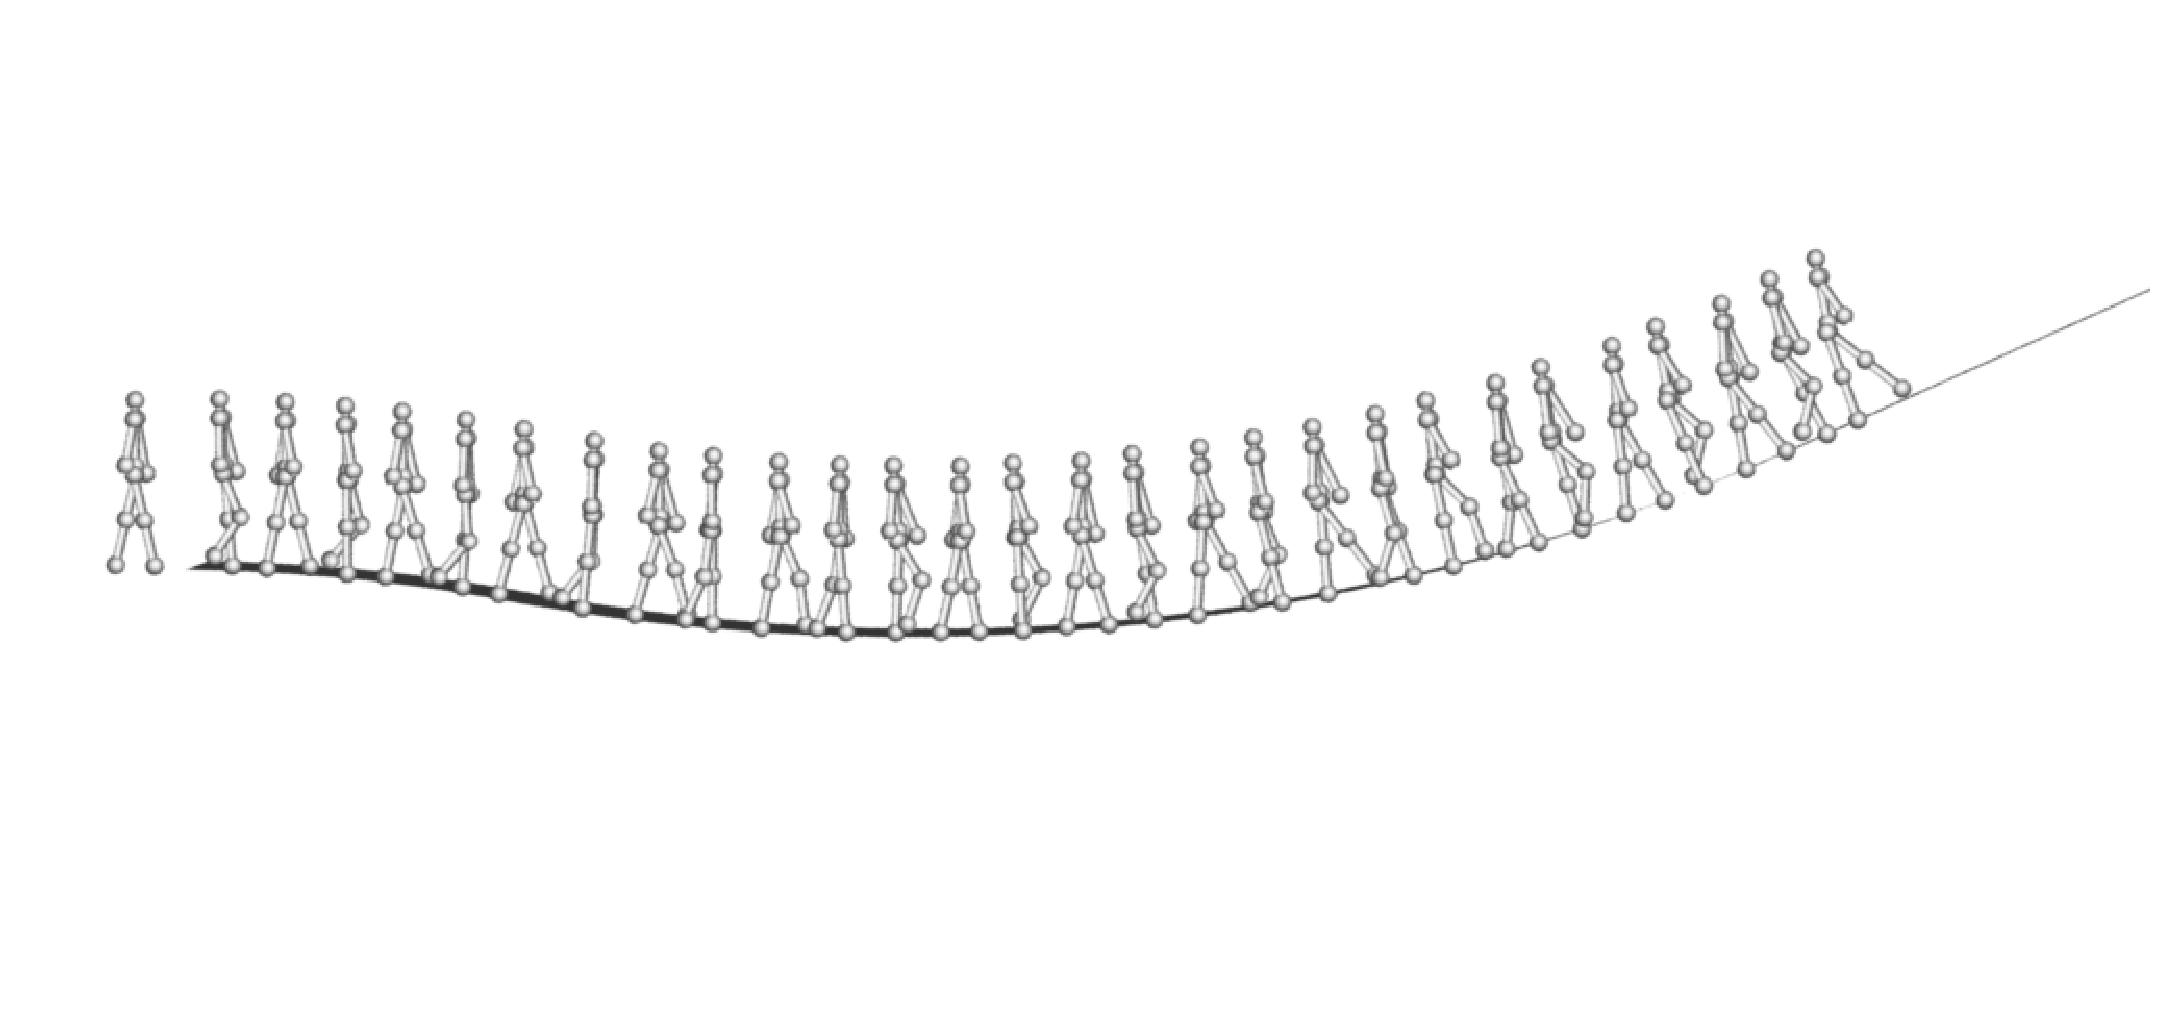
\includegraphics[width=0.7\textwidth]{vslope2}
    \caption{Continuous Varying Slope}
    \label{fig:vp1}
\end{center}
\end{figure}


\begin{figure}[!htbp]
  \begin{center}
      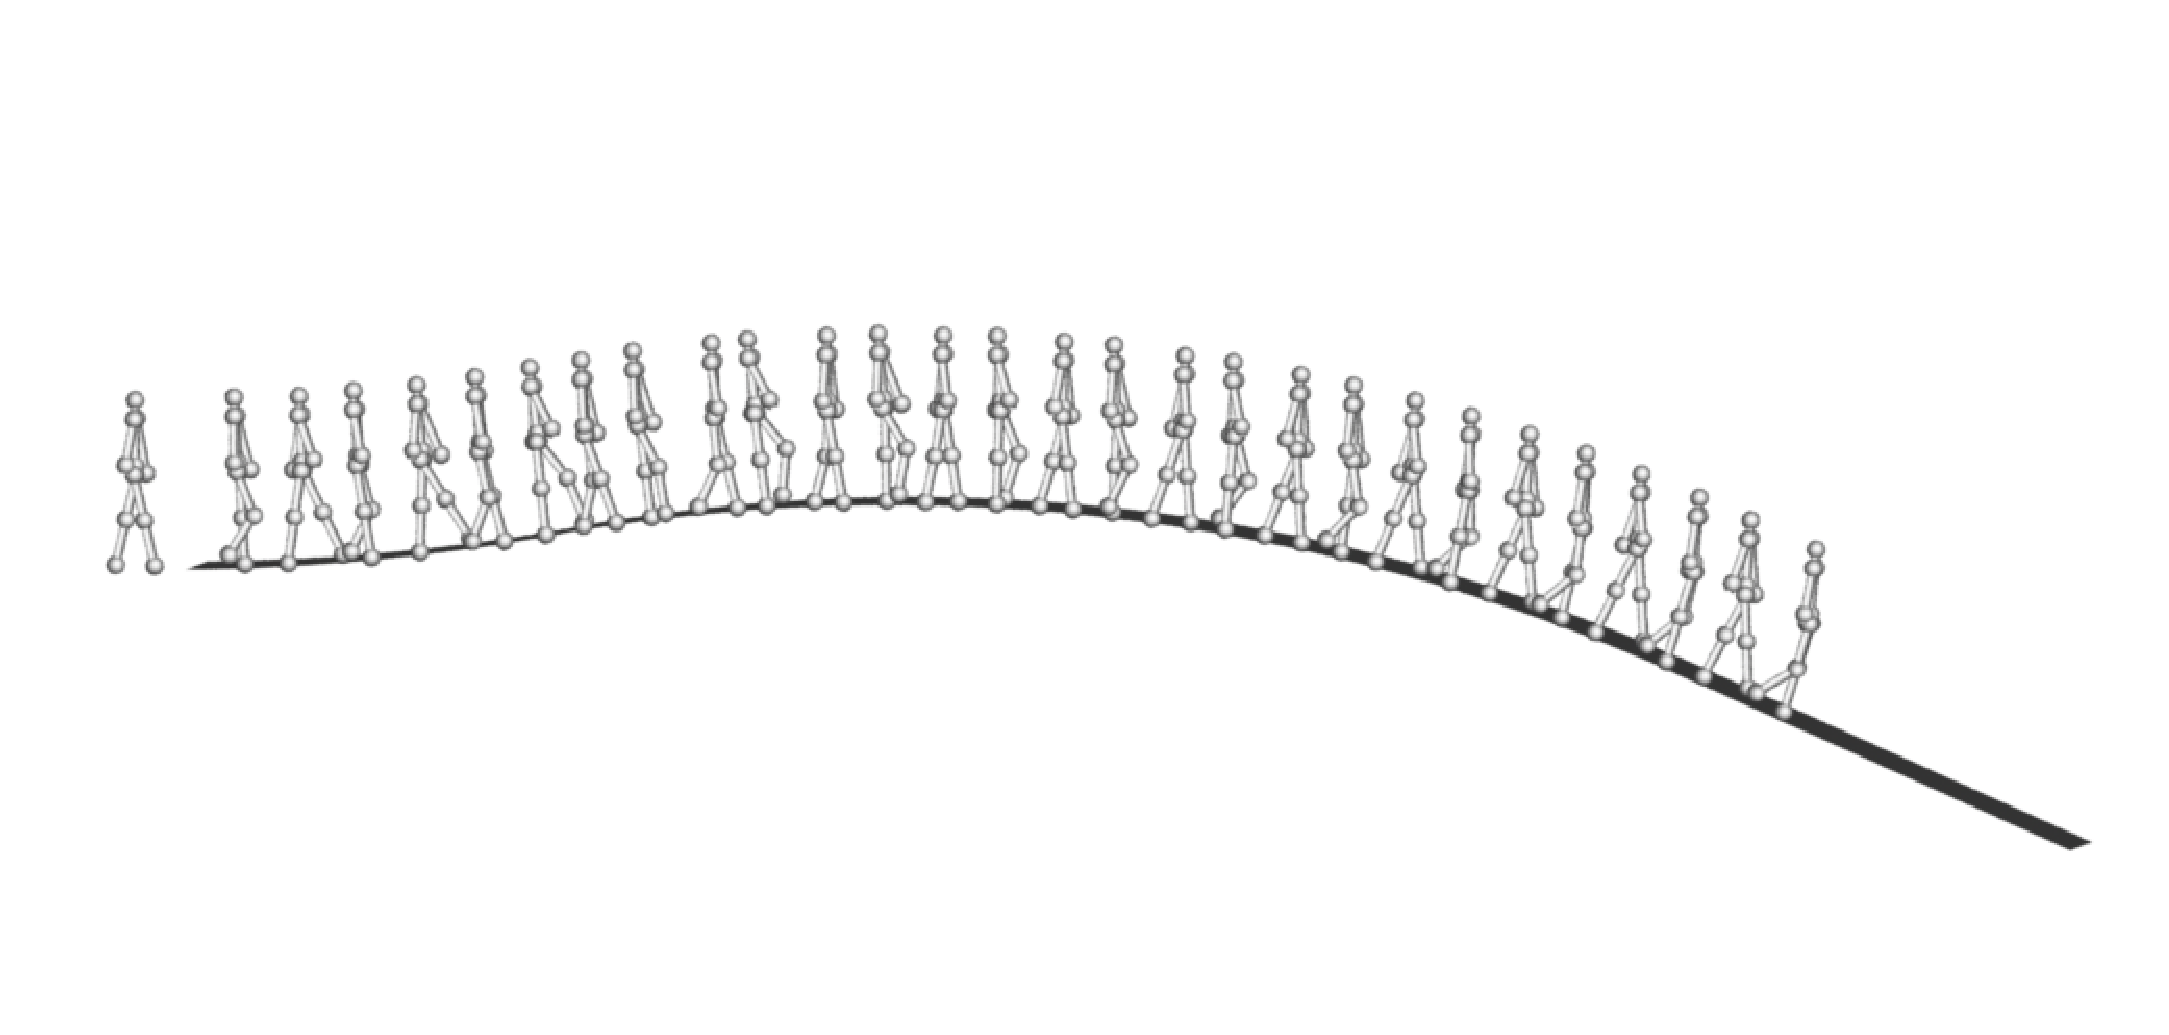
\includegraphics[width=0.7\textwidth]{vslope3}
    \caption{Continous Varying Slope}
    \label{fig:vp2}
\end{center}
\end{figure}


\begin{figure}[!htbp]
  \begin{center}
      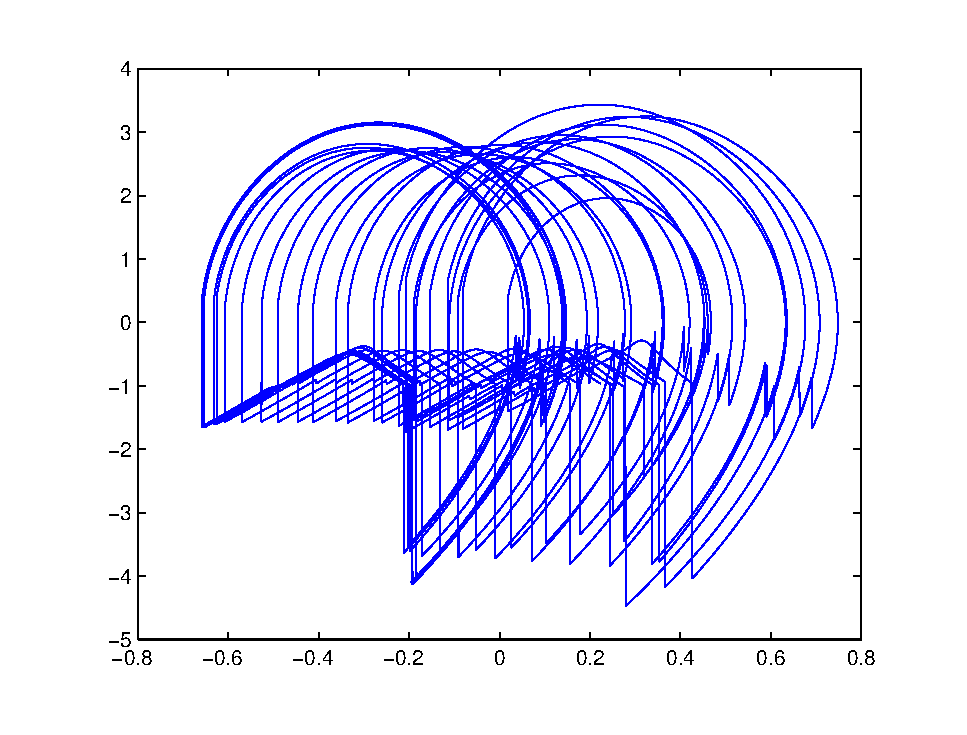
\includegraphics[width=0.7\textwidth]{vslope3phaseplot}
    \caption{Continous Varying Slope}
    \label{fig:vp2phas}
\end{center}
\end{figure}



Figure~\ref{fig:nonsmoothterrain1} and Figure~\ref{fig:nonsmootterrain2} show gaits on non-smooth terrain.
Figure~\ref{fig:diffterrain2} shows the phase plot of gaits in Figure~\ref{fig:nonsmootterrain2}, where different colors show different slopes.
\begin{figure}[!htbp]
  \begin{center}
      \includegraphics[width=0.7\textwidth]{terrain2}
    \caption{Non-smooth Terrain }
    \label{fig:nonsmoothterrain1}
\end{center}
\end{figure}

\begin{figure}[!htbp]
  \begin{center}
      \includegraphics[width=0.7\textwidth]{terrain3}
    \caption{Non-smooth Terrain coloured}
    \label{fig:nonsmootterrain2}
\end{center}
\end{figure}


\begin{figure}[!htbp]
  \begin{center}
    \includegraphics[width=0.7\textwidth]{Terrain3PhaseDifferentColor}
    \caption{The Phase Plot of non-smooth terrain}
    \label{fig:diffterrain2}
\end{center}
\end{figure}



\section{Verification}
In this section, we discuss stability, energy efficiency and the biological justification for the proposed approach. 
The stability is demonstrated by numerically approximating the basin of attraction of the passive walking model under environmental perturbations and under different initial conditions. 
The energy cost of each controller is evaluated with various gradient and offset action conditions. 
In order to link our results to the biological observations, we will analyse the captured motion data of a human walker adapting to environmental perturbations which are similar to those demonstrated in the above sections.
\subsection{Stability analysis}

The structural stability is analyse numerically by considering the basin of attraction of the passive dynamic walking model.
The improved stability of our proposed approach is demonstrated in Figure~\ref{fig:boa_plot} . 
The simulation runs from the foot strike phase (the bottom left corner of the plot) until it either converges towards the limit cycle or diverges.
The initial conditions, which are the starting angular velocity of the leg for this case, are incrementally increased and decreased and the result is re-plotted until the motion is unstable. 
Only stable cycles are displayed.
The passive walker is stable with a gradient of 0.06 radians (Figure ~\ref{fig:boa_plot} (a)) but considerably less stable with a gradient of 0.03 radians (Figure ~\ref{fig:boa_plot} (b)). 
In Figure ~\ref{fig:boa_plot} (c) the stability of the system (as demonstrated by the size and shape of the basin of attraction) is greatly improved by coupling the \cpg. 
By applying the offset group action to the system in Figure ~\ref{fig:boa_plot} (d), the step size is adjusted to compensate for the change in gradient, which improves the stability further.

\begin{figure}[htbp]
\centering
\subfigure[Passive walker (0.06 radians)]{\resizebox{0.45\linewidth}{!}{\includegraphics{BoASpeedStable}}}
\subfigure[Passive walker (0.03 radians)]{\resizebox{0.45\linewidth}{!}{\includegraphics{BoASpeedPassive}}}
\subfigure[$+$Neural control]{\resizebox{0.45\linewidth}{!}{\includegraphics{BoASpeedNeural}}}
\subfigure[$+$Group action]{\resizebox{0.45\linewidth}{!}{\includegraphics{BoASpeedGroup}}}
\caption{\label{fig:boa_plot}Sensitivity analysis demonstrating the stability of the walking model under perturbations of initial angular velocity.}
\end{figure}

 
\subsection{Energy efficiency}
Since the passive walker uses no energy, the energy consumed in the system depends on the control variables uout  and ulocal only. 
We compute the individual cost of transport \citep{collins05a} of each controller as $\int|\omega \uout(\x_c)|$ for the neural controller and $\int|\omega \ulocal(\x)|$ for the local controller, where $\uout(\x_c)$ and $\ulocal(\x)$ are local and global invariant control effort and $\omega$ is the angular velocity. 

Since these may affect each other, the resultant cost may be less than the total energy applied by the controllers. 
If these two controllers have independent actuators, then we should consider the sum of the absolute controller torque output from the controllers. 
We assume that there is only a single actuator, implying that only the resultant torque is appropriate.
Therefore the resultant (net) cost of transport $\cet$  applied by the controllers in our method  is described by the following formula:
\begin{equation}
\cet = \int | \omega \left(\uout(\x_c) + \ulocal(\x)\right)| \mathit{dt}.
\end{equation}
We evaluate this energy over a stable limit cycle by varying the gradient and the value of the offset controller in Table~\ref{tab:energy}.
\begin{table}[htbp]
 \centering
 \begin{tabular}{|l|l|l|l|l|}\hline
  \multicolumn{2}{|c|}{}&\multicolumn{3}{|c|}{\textbf{Cost of transport} $\cet$}\\\hline
  \textbf{Gradient} (rads)&\textbf{Offset} $r$&\textbf{Action cost}&\textbf{Neural cost}&\textbf{Net cost}\\ \hline
  0.060&0.000&0.000&0.021&\textbf{0.021}\\
  0.030&0.000&0.000&0.020&\textbf{0.020}\\
  0.030&0.030&0.030&0.021&\textbf{0.028}\\  
  0.000&0.000&0.000&0.029&\textbf{0.028}\\
  0.000&0.030&0.030&0.020&\textbf{0.026}\\
  0.000&0.060&0.061&0.021&\textbf{0.047}\\
  0.000&0.080&0.081&0.021&\textbf{0.068}\\
  0.020&0.080&0.081&0.021&\textbf{0.065}\\\hline
 \end{tabular}
 \caption{\label{tab:energy}Cost of transport for the global and local controllers and of the system as a whole.}
\end{table}
 Applying the offset action corresponds to altering the step size of the walking model. 
 We observe that the energy cost associated with applying the Lie group action increases linearly with the offset value. 
 The energy cost of applying the neural controller seems to be relatively constant. Note that the optimal solution for planar walking is to use an offset action of 0.03, which results in a smaller step size. 
 Compared with a state of the art real robot walking on a plane \citep{collins05a} with no local controller, our method uses approximately half the energy, probably due to the lower dimensionality and lack of damping in our system.
\subsection{Biological justification}
In order to provide a biological justification, we performed a simple experiment by capturing the walking motion of a single person using a commercial grade motion capture system
The participant walked on a calibrated mechanical treadmill under two separate environmental conditions in three increments. 
We varied the speed using the treadmill settings and the elevation by lifting one side of the treadmill. 
The motion of the walker was captured for a minute under each condition. 
The resulting data was cleaned from noise and smoothed before analysis.
\begin{figure*}[htbp]
\centering
\begin{tabular}{cc}
\begin{minipage}{0.2\linewidth}
  \subfigure[]{\resizebox{!}{6cm}{\includegraphics{sagital}}}
\end{minipage}&
\begin{minipage}{0.8\linewidth}
\begin{tabular}{cc}\hspace{0.0cm}
  \subfigure[Speed change]{\resizebox{!}{3.2cm}{\includegraphics{ankle_timescale}}}&
  \subfigure[Mean speed cycle]{\resizebox{!}{3.2cm}{\includegraphics{mean_ankle_timescale}}}\\
  \subfigure[Elevation change]{\resizebox{!}{3.2cm}{\includegraphics{ankle_elevation}}}&
  \subfigure[Mean elevation cycle]{\resizebox{!}{3.2cm}{\includegraphics{mean_ankle_elevation}}} 
\end{tabular}
\end{minipage}
\end{tabular}
\caption[Biological justification]{\label{fig:justification}On the phase plot, we can demonstrate how a real human adjusts to changes in the environment. The red, green and blue lines represent data captured under different elevation or speed conditions. $q$ is the angle in radians between an orthogonal to the horizon and the line from the hip to the ankle of one leg.}
\end{figure*}
In Figure ~\ref{fig:justification},  we show the results of plotting the angle against angle gradient in the sagital plane between a vertical direction and the line from the hip to the ankle of the participant, which approximately corresponds to the controlled parameter in our dynamic system. 
Minimal data processing was necessary to tease out this result — a standard 1-D filter to remove small local peaks, and the entire path was divided into motion segments and aligned by finding peaks in the cycle corresponding to the foot striking the ground.

The mean cycle clearly shows that a form of global invariant preserving motion adaptation took place when the environmental conditions changed. 
Changes in treadmill speed clearly caused the participant to increase the energy in the dynamic system, analogous to the energy scaling action. 
When the elevation of the treadmill was altered, the participant adapted by both increasing the step size transformation (presumably in order to maintain the same speed) and adapted to the change in gradient by applying an offset operator.

There are distinct differences between a fully actuated biological human system and the passive walking model.
A human will adopt an ankle strategy to minimize the strike momentum and therefore reduce energy loss, which explains why there is no significant spike in the real limit cycle when the foot strikes the ground. 
In spite of this, our measured results mirror the synthetic results remarkably well.






